% Created 2020-11-21 Sat 14:21
% Intended LaTeX compiler: pdflatex
\documentclass[12pt,titlepage]{article}
\usepackage[utf8]{inputenc}
\usepackage[T1]{fontenc}
\usepackage{graphicx}
\usepackage{grffile}
\usepackage{longtable}
\usepackage{wrapfig}
\usepackage{rotating}
\usepackage[normalem]{ulem}
\usepackage{amsmath}
\usepackage{textcomp}
\usepackage{amssymb}
\usepackage{capt-of}
\usepackage{hyperref}
\usepackage{parskip}
\usepackage{listings} \usepackage{color} \definecolor{dkgreen}{rgb}{0,0.6,0} \definecolor{gray}{rgb}{0.5,0.5,0.5} \definecolor{mauve}{rgb}{0.58,0,0.82} \lstset{frame=tb, language=Java, aboveskip=3mm, belowskip=3mm, showstringspaces=false, columns=flexible, basicstyle={\small\ttfamily}, numbers=none, numberstyle=\tiny\color{gray}, keywordstyle=\color{blue}, commentstyle=\color{dkgreen}, stringstyle=\color{mauve}, breaklines=true, breakatwhitespace=true, tabsize=3}
\usepackage[style=verbose,backend=bibtex]{biblatex}
\addbibresource{local.bib}
\usepackage[english]{babel}
\usepackage[T1]{fontenc}
\usepackage{setspace}
\usepackage[AUTO]{babel}
\usepackage[hyperref,x11names]{xcolor}
\usepackage[colorlinks=true,linkcolor=SteelBlue4,urlcolor=Firebrick4]{hyperref}
\date{\today}
\title{}
\hypersetup{
 pdfauthor={},
 pdftitle={},
 pdfkeywords={},
 pdfsubject={},
 pdfcreator={Emacs 27.1 (Org mode 9.3.7)}, 
 pdflang={English}}
\begin{document}

\begin{titlepage}
   \begin{center}

       
\includegraphics[width=1.0\textwidth]{./thesis_images/university.png}

       Scuola di Ingegneria Industriale e dell’Informazione\\
       Dipartimento di Elettronica, Informazione e Bioingegneria\\
       Corso di Laurea Magistrale in Computer Science and Engineering \\
       \date{\today}



       \vspace{2.8cm}
       \textbf{Workflow based orchestrations of serverless workloads with ephemeral statestore}

       \vspace{0.5cm}

       \vfill
       \vspace{1.5cm}

       \textbf{Supervised by:}
       Prof. Alessandro Margara

       \vspace{0.5cm}
       \textbf{Submitted by:}

       Nandaja Varma Nandakumar

       894333

       \vspace{1.0cm}
       Academic Year 2019/2020

   \end{center}
\end{titlepage}

\begin{abstract}
Serverless Computing is an up and coming Platform as a Service(PaaS) offering
where the cloud provider manages and allocates
resources needed to keep the application running. This lets the developer focus on the application development
and not on server maintenance. Alongside off loading the provisioning and
maintenance of the server, Serverless computing also reduces resource waste
by scaling up and down the allocation depending on the load and the
configurations. The users only pay for the resources that were used by the
application thereby saving huge operational cost on their infrastructure
hosting.

Although Serverless might sound like the holy grail of application hosting, the
current state of art technology fall short in several places to meet the industrial
requirements. Data intensive applications, streaming applications, and
distributed computing are some of the fields that could be benefited heavily by
implementation on Serverless platforms in terms of ease of development,
efficiency and cost. But all the existing platforms offer very
poor performance in these fields and works mostly via workarounds and numerous
third party tools.

This thesis analyses the Serverless paradigm in depth,
pointing out the reasons for this reduced adaptability. To solve these issues, we propose a lightweight
extension to OpenFaaS, an Open Source Serverless platform, that provides
flexibility, scalability and adaptability, while making sure not to violate the notion
of functions. Our implementation tries to reduce the operational gap between the
industrial applications and theoretical ideas put forward by researches in the past few years.
This thesis also offers a deep study of the full potential and limitations of
Serverless thereby making it clear to the reader why more innovation is
necessary in this field.

  \par
  \medskip % Add a small space between the two abstracts
  \medskip % Add a small space between the two abstracts
  \pagebreak
\begin{center}
  \textbf{Sommario}\par
\end{center}
Le piattaforme di Serverless Computing sono soluzioni emergenti Platform as a Server (PaaS) dove il fornitore di servizi cloud gestisce e alloca le risorse necessarie per mantenere in esecuzione l'applicazione. Ciò consente allo sviluppatore di concentrarsi sullo sviluppo del software
e non sulla manutenzione del server. Oltre a diminuire il carico di lavoro per il provisioning e
la manutenzione del server, questa tecnologia riduce anche lo spreco di risorse
aumentando o diminuendo l'allocazione a seconda del traffico e delle
configurazioni. In questo modo l'utente paga solo per le risorse che sono state utilizzate dall'applicazione risparmiando così enormi costi operativi sulla loro infrastruttura
ospitante.

Sebbene il Serverless Computing possa sembrare il santo Graal dell’hosting di applicazioni, attualmente le tecnologie all’avanguardia non sono all’altezza in molti casi di soddisfare i requisiti industriali. Applicazioni con uso intensivo di dati, applicazioni di streaming e di elaborazione distribuita sono alcuni dei campi che potrebbero trarre grandi vantaggi da un’implementazione su piattaforme Serverless in termini di facilità di sviluppo, efficienza e costo. Tuttavia tutte le piattaforme esistenti offrono soluzioni alternative combinando strumenti di terze parti, con scarse prestazioni.

La presente tesi analizza in profondità il paradigma Serverless, sottolineando le ragioni della sua ridotta adattabilità. Per risolvere questi problemi, proponiamo una leggera estensione di OpenFaaS, una piattaforma Serverless open source che fornisce flessibilità, scalabilità e adattabilità assicurandosi nel contempo di non violare la nozione di funzioni. La nostra implementazione cerca di ridurre il divario operativo tra le applicazioni industriali e le idee teoriche prodotte dalle ricerche negli ultimi anni. Questa tesi offre anche uno studio approfondito del pieno potenziale e dei limiti del Serverless Computing, rendendo così chiaro al lettore la necessità di innovazione in questo campo.

\end{abstract}



\setcounter{tocdepth}{5}
\tableofcontents

\listoffigures
\listoftables

\section{Introduction}
\label{sec:orgffdd62d}

Serverless can easily be considered as the new generation of Platform as a
Service(PaaS). It is a deployment solution where instead of having continuously
running servers, application instances come up and execute on predefined events.
While the developers worry about
the logic of handling the requests/events, the infrastructure provider takes
care of receiving the request, responding to them, capacity planning, task
scheduling, and operational monitoring \hyperref[ref:1]{[1}]
This has huge economical and architectural implications that is
still waiting to be explored in its full potential.

In the current industrial workloads, Applications are increasingly becoming data intensive
day by day paving way to adopt several resource heavy tools to do stream
processing, distributed processing, etc. More than often CPU and memory loads in
these machines tent to vary a lot and rather than having a dedicated server to accommodate the whole range
of requirements, it makes perfect sense to convert it into a Serverless workload
thereby saving up on operational cost, resource waste, and ease of development.
However, the current commercial offerings of Serverless do not work
very well with such workloads.

This is mostly due to the sheer
nature of the Serverless paradigm of being completely stateless, thereby forcing
the developers to use external block storages for data store and communication.
By the design of it, Serverless applications are deployed as isolated entities
which are hard to address directly via the network. This makes the composition
of functions a tad bit complicated. The most commercial Cloud Service Providers
currently offer wrapper solutions to workaround the composition problem. A very
notable commercial solution here is AWS stepfunction. AWS stepfunction provide
an API to define function compositions, which eventually get executed in AWS
Lambda, the pioneer in serverless platforms. Other than enforcing vendor lock in
to AWS, stepfunction comes with numerous limitations like 20s timeout on the API
gateway, 5 minutes limit to lambda execution, a limit of 2 executions per second
etc.

Another major requirement usually for heavy multi-staged processing pipelines is fault
tolerance. If at all a stage fails, the system should be able to restart from
where it failed with the correct intermediate data and complete the workflow. In
orchestrations like stepfunction where data is passed over the gateway among
each other, if a failure occur the processed data till the failure function is
gone for good. This makes the system unreliable for certain heavy load applications.

In this thesis, we propose an approach to improve the performance of big data workloads
on the Serverless platform by introducing the provision to provide a
computational graph to the Serverless platform which defines the control flow
and data flow in the orchestration. The intermediate data transfer between the
functions will be taken care with the help of maintaining a scalable in memory
distributed cache and storing the intermediate data in them as ephemeral data.
Our system also provides fine grained control over resource allocation and
scaling rules for each individual function. Alongside, it provides extensive
monitoring, function level tracing and visualization, and out of box setup and
deployment. Because of the usage of the intermediate ephemeral storage and fine
grained monitoring the system provides automatic fail overs. Meaning, if at any
step the operation fails, the pipeline will be able to
restart from the point of failure without redoing the whole process till then.
The system will offer an at-least-once guarantee in the request handling. This
is mostly because of the message queue that is being used by the FaaS system we
built on called NATS streaming \hyperref[ref:47]{[47}]. 

It is worth mentioning that our implementation focuses on reducing the gap that currently
exists with a lot of research ideas and the industry level applications, making
it an easily adaptable solution. We propose a very secure and multi-tenant implementation of a
state-ful Serverless setup which can be easily used for production quality
applications. The possibility to efficiently do application performance and
usage monitoring makes fine grained billing an out of the box functionality.

Managing intermediate data via additional infrastructure instead of altering the
stateless nature of the function was a conscious choice. The serverless computing abstraction,
despite its many advantages, exposes several low-level operational details that
make it hard for programmers to write and reason about their code \hyperref[ref:4]{[4}]. This is
related to misusing/misunderstanding state in serverless environment. Since
the same function is reused again and again to avoid latency, the cache or state
persists across invocations leading to faulty results. If the state store is
handled by an external party mapping to the invocation id, a lot of this faulty
management can be handled.

As for the implementation, we proceed by extending an existing, widely used
Serverless platform called OpenFaaS so as to make it readily adaptable as a FaaS
infrastructure for production quality applications. As for the function
composition, we use an existing library faas-flow to support event driven
workflow based function composition pattern. We make sure that the notion of a
function or serverless platform will not be violated in this process since with
the current state of art of infrastructure deployment, autoscaling and
concurrency happen by leveraging the notions of statelessness and
functional coding. The proof of concept of our solution was successfully
implemented \hyperref[ref:59]{[59}] and has been Open Sourced.

There has been several academic researches on ephemeral autoscaling storages in
the past couple of years. Pocket project is one that has received appreciation
and we will be analyzing this platform in depth. Our thesis implementation
adapts an existing ephemeral storage platform.

Using our proposed Serverless setup, we try to efficiently run an
Extract-Transfer-Load(ETL) workload on streaming data. ETL basically is a
pipelined workflow that involves receiving data
from source, cleaning and transforming it, and loading it to a sink. We will
split the whole operation into multiple functions as per the Serverless notion
and have them communicate data internally via the ephemeral data store
to complete the pipeline thereby reducing the latency and external bottlenecks.

This document describes more on Serverless paradigm, the shortcomings of it, the
ones we are trying to solve, our solution and evaluation. It is split into
several sections as follows:

In Section 2, we go a bit in depth to understand the history of cloud
infrastructure and the technological innovations that led to Serverless
paradigm. We also look in detail at the characteristics and nature of
Serverless. We look at some commercial Serverless offerings and understand how
in the programming world Serverless has affected even the way of coding.
We will also see what limitations it holds at its current state of art and
the problem statement of the thesis.

In Section 3, We elaborate on the proposed solution for our Serverless setup going
into detail about how certain crippling limitations can be overcome.

In Section 4, we present the implementation of the system including the architecture and
the tools used.

In Section 5, we go on with the evaluation of our system.

In Section 6, we look at the current state of research in the field of
Serverless technologies and the related works.

In Section 7, we lay down the future works that the system has got planned
moving forward.

We conclude by pointing out what went well and what did not with our solution in
Section 8.

\section{Background and Motivation}
\label{sec:org45fae5e}
The term Serverless has been vaguely thrown around the domain of cloud
infrastructure in the past decade as the breakthrough resource(and hence money)
saving tool that lets the developers focus on application logic rather than the
deployment and server maintenance. However, it is often hard to define
what exactly serverless is since the service offering tend to change based on
the cloud provider and the interpretations of the users. It is fair to say that
serverless is a huge leap in the direction of using computational power as a
resource which is paid for, according to the usage.
Although the terminology is irrelevant, we will be focusing on the serverless
offering called Function-as-a-Service(FaaS) where the cloud providers offer a
platform to which we can upload our application code to(complying to the API
rules) and get uninterrupted service of the same at an endpoint no matter how
the traffic or data load might be. Paying only for what resources has been used adds to
the attraction of the domain.
In this section, we will understand more about this technology, the
popular commercial offerings of the same, and its limitations and the current state
of research.
We will also analyze the popular data processing and streaming pipelines in the
industry these days and why Serverless computing fall short in being the right
tool of development and deployment in some cases.
\subsection{Evolution of cloud resource management}
\label{sec:org91b7f4b}
In the past three decades, software deployment and infrastructure management has
seen a lot of innovation and evolution. Before diving into the current
industrial standards, it is important to understand the evolution in this field
to get a better grasp on the technological innovations that brought about this change.


\subsubsection{Dedicated servers}
\label{sec:orgb81bdb6}
Even as recent as fifteen years ago, using dedicated servers was the industry standard for deployments. Dedicated servers
are physical machines. The general practice was to have server racks on the premise
of the company which are maintained by system administrators and all your
software is
hosted there. Although this method offers advanced security and high
availability, it is often common that a lot of physical resources were
underutilized and each resource was for single client. Not to mention the
environmental impact of the reserved heavy hardware which leaves a heavy carbon
footprint and e-wastes.


\subsubsection{Dedicated virtual machines(BaaS)}
\label{sec:org3fd3c95}
Virtualization technology changed the face of software infrastructure by decoupling
applications from the underlying hardware. Virtualized servers are not physical
machines, they are a software construct. Virtual servers run on dedicated
servers, the resources of which are divided between several virtual servers.
To get slightly technical, virtualization usually involves installing a virtualization software(Hypervisor) on an
existing operating system and then having multiple operating systems on it,
sharing all the resources of the host operating system, yet providing
great security and isolation.

\begin{figure}[!h]
    \caption{Virtualization through hupervisors}
    \centering
    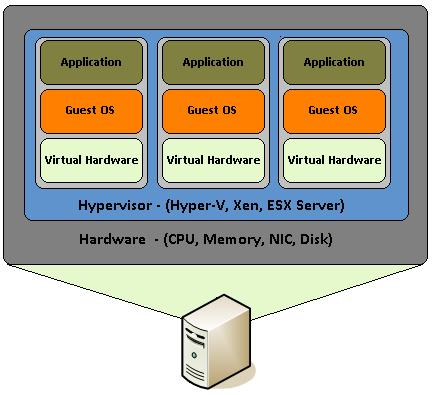
\includegraphics[width=80mm]{./thesis_images/virtual_machines.JPG}
    \label{fig:testing the label}
\end{figure}


Although applications hosted on the virtual machine suffer from a heavy
input/output and network overload because of the added layer of indirection,
this technology reduces the resource waste to a great extend. The enterprises could partition their hardware into
multiple virtual machines and have different hosting and computation in each of
the them. System administrators started splitting up their bare metal resources
among multiple Virtual Private Servers(VPS) by the help of virtualization
software. Each VPS would give you the feeling
of having a real system although it is a virtualized system which is sharing the
resources with other VPSs. This reduced a lot the amount of work and energy spent on
maintaining server racks along with the terrible underutilization of resources.

More and more companies started adapting this technology and in early 2006
Amazon Web Services(AWS) re-launched themselves as a platform that offers
computing and storage space to developers and enterprises on an on-demand basis
revolutionizing how companies were designing their system architecture. Soon
after Google and Microsoft followed suit with their cloud infrastructure
platforms offering similar services. All these providers function by maintaining
huge, dedicated server farms across the globe to provide the necessary resources
to the customers.

These kind of services, generally called as Infrastructure as a Service(IaaS) or
Platform as a Service(PaaS), went through a
series of changes during the past decade. On-demand compute instances to
completely managed deployment services(eg: Google App Engine), Pay per use block
storages(AWS S3) to fully managed dedicated relational databases(Google Cloud
SQL, AWS RDS, etc.) a lot of really efficient and interesting services started
to be available for the developers disposition. The billing scheme of these
services also started to be quite flexible even allowing a per second billing
plan in the past couple of years by Google.

It is also worth noting that with the advent of virtualization, the job profiles
in several companies shifted from having a system administrator role to
having profiles called DevOps(development and
operations) who are application developers focusing on the provisioning of the
virtual machines to deploy their applications. Although IaaS solved a lot of
hassle around infrastructure provisioning, the systems and load of the
applications still remained independent. Applications always had dedicated virtual machines
even if the load/traffic to and fro the application is not constant. This meant that a
lot of resources were still being wasted.

\paragraph{Linux Containers}
\label{sec:org1514fcb}
A game changer in the world of virtualization was containerization. Containers
are yet another packaged computing environment that combine various IT
components and isolate them from the rest of the system just like a virtual
machine would. It was developed to solve a lot of problems with virtual
machines. The purpose of the containers is to encapsulate an application and its
dependencies within its own environment. This allows them to run in isolation
while they are using the same system resources and the same operating system.
Since the resources are not wasted on running separate operating systems tasks,
containerization allows for a much quicker, lightweight deployment of
applications. Each container image could be only a few megabytes in size, making
it easier to share, migrate, and move. Figure \ref{fig:vm_vs_containers} shows the difference in the
isolation levels of containers and virtual machines.
Even though Linux Containers \hyperref[ref:5]{[5}]
have existed for a very long time, in the past decade, containers were made a
lot more approachable and adaptable as a
technology by the advent of communities like Docker and rkt.

\begin{figure}[!h]
    \caption{Virtual Machines Vs Containers}
    \centering
    \includegraphics[width=80mm]{./thesis_images/VM_image.PNG}
    \label{fig:vm_vs_containers}
\end{figure}

The light weight of the containers
made it the ideal candidate for running applications. What makes container based deployments special
as opposed to the ones deployed directly on the host is the consistency of the environment. The application
execution environment can be recreated and ported from one system to another without affecting the functionality
of the application or having to reinstall the whole binary dependencies on the new machine. Reproducability of the
production environment even in the local exactly, meant that the development/testing cycle became much more efficient.
The isolated package of the application, enveloped as a container image, is
agnostic of the operating system it runs on opening new possibilities for the
deployment. One could also limit and fine tune the resources used by a running
containers giving a lot more control over the application.

\paragraph{Autoscaling}
\label{sec:org64de244}
The ease in which one can limit the resources and tweak the runtime parameters externally contributed heavily
to the service offering called autoscaling which basically meant resources for an
application runtime were added or removed as per the usage. All the commercial
cloud providers started offering the aforementioned service in different
flavors. Autoscaling on EC2 or Google Compute, AWS Fargate, etc. are some examples.

In the past two years, innovations have taken a leap in the field of isolation
environments, introducing solutions like AWS Firecracker, Cloudflare workers,
etc. to the community. These solutions aim at mitigating the shortcomings of
Containers which we will discuss in Section 2.2.4

\subsubsection{Serverless}
\label{sec:orgedaf2ad}
Like mentioned earlier, in the past two years the terms Serverless and Function-as-a-Service are quite
often used interchangeably. In terms of the resource reservation, Serverless can
be considered as a platform as a service solution that scales. Your application
will always have enough and only enough resources dedicated to it. It will scale
up and down based on the load and traffic and the developer only pays for the usage.
This paradigm of autoscaling has been hence applied even to database storage
solutions by major cloud providers such that even the block storage is allocated
based on usage and there will be a burst of reservation as soon as a certain
limit is reached.
The pioneers of this technology can be considered as the proprietary service
Lambda by Amazon Web Services\hyperref[ref:6]{[6}]. Several other cloud providers followed suit
with similar platforms specific to their infrastructure.
The nature of serverless makes it attractive for both developers and the cloud
providers since in the case of former, it means paying much less and in case of
the latter, it means they can easily provide shared tenant resource allocation
units.

We will dive more into the properties and nature of the solution
Function-as-a-Service(FaaS) in the following session.

\subsection{FaaS}
\label{sec:orgc45b248}
So far, we have covered the infrastructure management style of FaaS or
Serverless in general. Let us discuss in detail the specifics of the
hosting platform that provides the FaaS functionality.

Most FaaS platforms being closed source, provides the client API for developers
to supply a package including their code and dependencies to. Most platforms
supports a limited set of programming language runtime although it is usually
possible to do workarounds to deploy custom runtime. Behind the screen,
the platform containerizes the application and deploy it so as to get triggered
via pre-defined hooks specified by the developer. The infrastructure also provides endpoints or
interfaces to specify the maximum and minimum CPU and memory allocated for the
application, the maximum timeout for the application(although there is a
hard bound on this imposed by the infrastructure provider usually). To
understand the flow of FaaS workloads, it is important to be aware of the
following properties of the platform.

\subsubsection{Properties of FaaS}
\label{sec:orgf825e17}
\paragraph{Statelessness}
\label{sec:org9da52ea}
Statelessness in deployments is a conscious decision that was taken during the
conception of the Serverless infrastructure model to make the management of the
platform straight forward and less cumbersome. Statelessness simply means that
the applications that are to be deployed on the said platform exists as
independent functions that are pure in nature. As in, the same data input given
to the function always produces the same output at any point in time. This is
what is termed as the lack of side effects. The data source and sink of
the function can be any supported platform or tool as per the requirement, but
there will not be any intermediate state or cache for the function. This means that
the function at any execution will have no information about the previous
execution unless explicitly specified.

The main advantage with this method for the infrastructure manager is pretty
obvious. The fact that there are no volumes necessary to store any internal
state means that the function can be scaled up and down independently and the
whole infrastructure can stay elastic. Along with this, the provider can
schedule the function in any node in the cluster that they use to host the
application, move it around as per the usage burst, have multi-tenant
deployments in a single machine ensuring the proper isolation for maximum
profitability, and the list goes on.

In short, the notion of function is of prime importance in a
Function-as-a-Service workload like the name suggests.

\paragraph{Triggers}
\label{sec:org75016d0}
The functions that are hosted on a FaaS solution need to get triggered on a timely
basis or based on an event. Usually most cloud providers provide more than a few
ways to trigger the functions which the developer can choose from. Some of the
most common triggers for FaaS applications are
\begin{itemize}
\item HTTP requests: An endpoint will be provided by the platform for the function that was deployed.
\end{itemize}
This endpoint can be called as an REST API endpoint and the event handler of
the function will get the payload from the call.
\begin{itemize}
\item Data arrival in a storage or data broker system: This is the most popular and heavily used triggering mechanism in FaaS. The idea
\end{itemize}
is that the function gets triggered as soon as a new data arrives in whatever
format at a particular storage setup. This can be arrival of a file object in
the S3 block storage, arrival of streamed data in Kafka message broker system,
etc. This method is the most suited for big data and streaming data applications
since the function can be activated as soon as the new data is detected in the
source. Usually the FaaS infrastructure provide supports more than a bunch of
source storage to be used as the sources for the trigger.
\begin{itemize}
\item Cron: Another very common way to trigger function is based on a schedule. The
\end{itemize}
programmer can choose how often the function should be triggered on what days of
the week, month, year, etc.
\paragraph{Billing}
\label{sec:orge8a5956}
One of the most attractive features of the FaaS service is the 'pay for what you
use' policy. Billing model is an important constituent in the equation. Generally
the commercial cloud providers charge you on the amount of memory that was
reserved for the function, the execution time of the function in relation to the
number of invocations that the function incurred. In most of the platforms, the
developer can configure a maximum amount of memory that need to be dedicated to
a function during its invocation. To save on the billing, if the user reserve
less memory for the function, at the end of the day the execution time ends up
being longer and there will not be much notable difference in the money spent \hyperref[ref:7]{[7}]
Figure \ref{fig:lambda_billing} shows more on how billing varies as a function of execution
time \hyperref[ref:8]{[8}].
\begin{figure}[!h]
    \caption{Lambda cost by fucntion execution time for 100,000 executions}
    \centering
    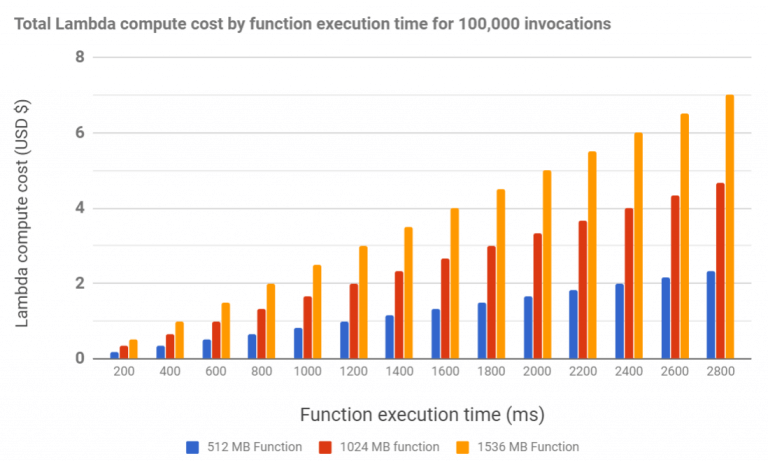
\includegraphics[width=80mm]{./thesis_images/lambda_billing.png}
    \label{fig:lambda_billing}
\end{figure}

When looking at the price per function invocation, currently at \$0.0000002 for
AWS Lambda and Azure Functions, it's very easy to get the impression that FaaS
is incredibly cheap (20 cents for 1 million invocations). However, the price
based on the number of invocations alone does not truly reflect the cost of
providing this sort of service like mentioned earlier. With the current AWS
Lambda price at \$0.00001667 for every GB-second used (Azure Functions cost
\$0.000016 for every GB-second), you can see how the cost mounts quickly.

Since the amount of allocated memory is configurable between 128 MB and 1.5 GB,
the total cost of function execution will vary depending on the configuration,
and the cost per 100ms of the execution time for the most powerful specification
will be roughly 12 times more expensive than the basic 128 MB option. Even with
this it is easy to see that FaaS is a pretty cheap option.

If we compare this to an IaaS solution we can realize the fact that FaaS is not
the right tool for all kind of applications. In the past couple of years, cloud
prices has fallen that keeping up a small cloud instances all the time would
cost comparable amounts. For example, the micro instance of EC2 costs \$4.25 in
average to keep it on for the entire month. In fact, simple math shows that
running a tiny EC2 instance would be cheaper than having a function running
continuously for the entire month. The saving comes up in the case of heavy yet
variable load applications. In this case, if we reserve the memory needed at the
peak load time, it is going to stay up with that capacity even during zero load
which is very expensive and a huge waste of resources. And this is where FaaS shines.


\subsubsection{How programming models are getting affected by this}
\label{sec:orga96a123}
\paragraph{Faas + Microservices}
\label{sec:org0f599b1}
In Software Systems Design, a widely discussed discussed topic is if to design the
application in a monolithic fashion or a micro-services fashion. Monolith is the
kind of design pattern where you have one big application doing multiple
functions and maintained as one solid stack. On the contrary, when one designs
their app in a microservices pattern, they will have to split up their application
into multiple smaller parts which can be independently built and deployed, and
yet working together with inter app communications. Both of these methods has
its advantages and challenges. When monoliths are easier to develop and
maintain, it can be very hard to test and manage due to the size, and usually if
one part is buggy, it tends to break the whole system. On the other hand,
microservices, since they work as independent units do not usually affect each
others working and can be very easily tested and maintained. It is although
often a very tedious task developing a system that fragmented and maintaining it
that way.  

With the advent of FaaS, a very interesting pattern has been adapted in the
industry. The pattern pushed microservices one step further. The idea is that
instead of having microservices that are available and on at all time, the huge
applications are split up into functions that can be deployed to a FaaS
infrastructure and triggered with the help of HTTP endpoints to act as a part of
web application setup. This method is very effective resource usage wise and
much easier to deploy and manage compared to vanilla microservices which have to
be built and deployed independently. A very notable reason for mixing up FaaS and
Microservice is that, Microservices usually embeds a local state alongside the application.
This is usually one or more provisioned volume in the local file system. This is
not possible in a purely FaaS based infrastructure. Deploying it alongside
microservices offer a lot functionalities.

\paragraph{Statelessness or Functional programming model}
\label{sec:org1a8b7d8}
Like mentioned earlier, the notion of function is very important for the
serverless platforms. It is intrinsically linked with functional programming. It
is very interesting to note that Amazon named their FaaS solution Lambda which
is a very basic concept of functional programming. Stateless clean functions
that produce no side effect was objectively the perfect choice for an
infrastructure solution of this scale.

What this change bought about is a thriving interest in functional programming
languages. A lot of the functional programming languages belonging to the LISP
family and some purely functional ones have seen a very increasing adaptation in
the past few years in Serverless platforms. Since these languages are perfectly
suited for stateless program it is only natural that they can be efficiently
used to code for this environment.
\subsubsection{Popular commercial offerings}
\label{sec:org980aa94}
Now that we have seen what makes FaaS an attractive field for cloud providers,
developers, and researchers alike, it is interesting to understand the popular
FaaS services out there.

AWS was the first big player in the field of Serverless introducing their
platform AWS Lambda in 2014 \hyperref[ref:9]{[9}]. Soon Google followed suite with their
cloud functions and then Microsoft and IBM entered the game with Azure Functions
and cloud functions respectively. In the past couple of years, Cloudflare \hyperref[ref:11]{[11}]
, Edge \hyperref[ref:12]{[12}], etc. has started providing similar services but the former
offerings still continue to lead the industry.

Although all the aforementioned commercial offerings contribute in strengthening
the vendor locked in nature of the FaaS paradigm, it is worth understanding to
see what kind of services a developer gets to have from each of these platforms.

The leading giants like AWS, Azure and Google tend to focus on configurability
and ease of use. Their FaaS platforms are easily triggerable from their other
cloud services, making it a very convenient yet monopolizing way of development.
To understand the nature of the leading commercial service providers, in this
section we go into looking at their characteristics.

\paragraph{AWS Lambda}
\label{sec:org2f644a1}
AWS lambda became publicly available in 2015 and currently dominates the
landscape of AWS lambda. AWS Lambda has a free-tier under which it covers first
1M function requests and 400,000 GB-secs per month. AWS Lambda functions can be written in a handful of
popular languages including Python, Javascript, Golang, C++, etc. The code is
supposed to be bundled as a zip file and uploaded using API operations provided
by AWS. One of the key issues that were noted often about AWS lambda at this
point is the dependency management. The dependencies are expected to be bundled
inside this zip file and there is a size limit to the zip. This is not a very
great way to manage dependent libraries especially for data processing
algorithms which deals with mathematical toolkits. Lambda provides guidelines
for the way code and dependencies are to be organized in the zip file.

The idea of statelessness takes an interesting approach in AWS Lambda. We
already saw how statelessness is a key aspect in FaaS platforms. To ensure that
the corrupted caches are lying around, AWS do not have any extra garbage
collecting processing. Instead it relies on the user not using any variables
while writing the function. This is a very functional way of programming indeed
but can be rather crippling when dealing with a lot of data. The way they
suggest the developers take care of this is by using an external block storage
like s3 to store these variables. The idea of AWS stepfunction was introduced
briefly in the introduction section. For enabling state in a stateless
architecture and orchestrate functions, AWS created Step Functions. This module
logs the state of each function so it can be used by subsequent functions or for
root-cause analysis.

Access management is managed by the IAM policies that are inherently used by AWS
to manage access to any cloud service. AWS Lambda provides you with the facility
to create your own custom IAM policies and attach them with your Lambda
functions. This allows permissions for AWS Lambda API actions, users, groups,
roles and resources.

Aws Lambda provides an API gateway and an HTTP endpoint to trigger the function
in standard way. Other than this AWS support a huge list of AWS services that
the developer can configure as the event source. Lambdas can also be invoked
using the AWS SDK.

Another aspect worth noting is concurrency support and the execution support.
AWS Lambda currently supports 1000 parallel executions of function instances and
each function has a maximum runtime of 15 minutes. It is worth noting that
concurrency often depends on the dependent resources that are used in the lambda
function which may not be scalable by nature. AWS Lambda generally increases the
number of concurrent functions running as soon as there is a rise in traffic. If
there is no predefined limit they keep increasing it by 500 per minute until the
demand is met.

\paragraph{Google cloud functions}
\label{sec:orgcc67c51}
Google Cloud Providers entire the FaaS race very recently, in July 2018.
Currently Google cloud functions do not support a lot of language runtimes. This
includes NodeJS, Python3, Go and Java 11. The functions written can be uploaded
to the service via the CLI, zip upload, inline editore, and cloud storages. So
far Google cloud provides the most flexible workflow in dependency management.
The developer just have to specify the dependent libraries in a package.json
file and the cloud provider installs them for you avoiding the heavy package
that needs to be uploaded like we saw in AWS lambda's case. This is really good
because if the developer is building the package with libraries included in a
Windows machine there will be huge incompatibilities for the package in the AWS
lambda.

For state or for sharing data between functions google cloud recommends similar
approach as of AWS Lambda, that is to use a cloud storage. The events for the
trigger can be triggered by HTTP requests, and a bunch of google storage
services like cloud storage, cloud pub/sub, cloud firebase, strackdriver
logging, etc. Access control is managed in a similar fashion to AWS, by using
IAM roles.

Google cloud functions really lags a bit behind when it comes to function
orchestration. It does not offer any kind of orchestration mechanism that for
the user to programatically chain functions via HTTP gateway.

When coming to the execution time, GCF have maximum hard limit of 9 minutes on
this. The concurrency of functions in GCF is measured at a per function level that at
an account level as opposed to AWS Lambda.

Fine grained scalability is not at its best yet on Google Cloud Functions. The
functions are known to be scaled pretty slow depending on their size. It is seen
to have a maximum cold start of around 500ms \hyperref[ref:10]{[10}], which is in fact
quite significant.

All in all Google Cloud Functions has to go a longer way to be a more flexible solution.

\paragraph{Azure functions}
\label{sec:org38b45f3}
Joining the world of Faas in 2016, Azure shines in a lot of places with its
Functions where Google Cloud Function falls short. To start with Azure functions
have a rich runtime almost comparable to AWS Lambda. They support a lot of very
popular languages. Contrary to AWS Lambda, Azure Functions provides you with
multiple options for deploying your function, such as GitHub, DropBox, Visual
Studio, Kudu Console, Zip deployment and One Drive.

The dependency management in Azure is very similar to AWS in that, the system
expects you to bundle all the dependencies together and upload it to the system.

In Azure, there is a tricky way to handle state by keeping static variables as
cache data. Although if someone needs persistent storage they will have to use
block storages.

While Azure Functions lets you control your function policies through Resource
Based Access Control. It is supported at Subscription and ResourceGroup. Though
at the moment, you can give permission to read/write access both to your
functions as read-only access disables some of the app’s features.

As for the function triggers, Azure too supports a bunch of Microsoft services.
But along with this, Azure lets you trigger the function using webhooks from
Github, external HTTP, APIM, function proxy and bindings. For the orchestration,
Azure functions provide Durable functions which basically is a bloated queueing
service to pass event triggers between functions. It is a weaker form of AWS
stepfunction.

The execution time is usually capped at 10 minutes. The number of concurrent
activity is apparently 10x the number of cores in the machine. Azure Functions’
free tier covers 1M requests and 400,000 GB-secs on the monthly basis.
Afterwards, you will pay \$0.000016/GB-secs and \$0.20 per 1M executions. Azure
functions have an embarrassingly long cold start period which is in the range of
3640ms on median.


\subsubsection{Where Serverless computing fall short}
\label{sec:org459a452}
Although serverless computing might sound like the silver bullet of the
deployment solutions, it is a field that is still being rapidly grown and
researched on. There are several staggering shortcomings for this technology
that makes it unsuitable for certain applications. The current offering have the
following noticeable limitations.
\paragraph{Lack of state}
\label{sec:orga784d7c}
As mentioned earlier, statelessness is a primary nature for serverless workloads
making it easy to deploy and port agnostic of the environment and server.
Hence serverless/auto-scaling paradigm generally push for a development style
involving no state to make the infrastructure simple, encouraging a functional
style of development. Although this can contribute to easily scalable and
parallelisable applications, it often limits the technology from being adapted
in applications that are data intensive.
The fact that serverless functions do not store any intermediate state requires
the application developers to use a block storage to store the data and state
after the execution. This basically means communication via slow storage and
adds a lot to the latency. This discourages the use of serverless in distributed
computing which is actually a domain that needs very fine grained communication
between the functions and usually a lot of resources are wastefully dedicated to
ensure high availability.

A function during execution has no clue of the previous executions and its
results. Which is something that is usually very basic for data analysis
operations. The developers in this case are forced to send the data after each
execution to a block store and retrieve the data from the block store before the
next execution. Other than the input output overhead and the network latency
this adds, it is a violation of the elastic nature of the Serverless
paradigm.

\subparagraph{I/O Latency}
\label{sec:orgc506a48}
Like was mentioned earlier, FaaS have had a lot of influences in the system
architecture and programming paradigms like would with any new infrastructure
management system. It is quite unfortunate though that, even with a paradigm
with such huge potential, FaaS is very conventional when it comes to its data
engineering architecture. Functions are run in isolated units separate from the
data or data store. This is actually a very huge system design anti-pattern
because Input/Output have and will remain to be a bottle neck even with heavy
memory and huge number of dedicated cores to a function. The pattern where the
data is taken to code as opposed to code to data adds to the latency, cost, and
inconvenience. For the clarity of the reader, an example of a code shipping
architecture is procedures that you run in databases. The code is moved to the
data than the other way around in this.

\paragraph{Coordination issues among functions}
\label{sec:orgab8bd36}
FaaS workloads are usually containerized by
the cloud provider to deploy it easily in their node pool or cluster. By nature,
docker containers are indiscoverable units that need to be opened up explicitly
to the network of the host machine. Meaning that, we cannot explicitly address
the docker container directly using an IP address or an endpoint. Cloud
providers do not open up the container to the network consider the potential
security issues this can cause and the necessity of state in this case. They
provide handles to communicate with the function or trigger-able entry points,
but no direct network addressability.

What this implies is that, if the developer has multiple functions that has to
be composed together to form a pipeline, rather than triggering each other
internally and directly, the developer will have to hack around by either
triggering it via an HTTP endpoint if the provider allows that, or like was
mentioned in the previous point via an external block storage, or other external
queueing systems they provide, etc. In either of these
scenarios, it is hard to avoid added latencies.

This makes FaaS particularly inefficient for applications like distributed
computing when it depends on very fine grained communication between the
functions. With FaaS we can only ensure very weak consistency across function
storages making it a pretty bad candidate. What this also means is that there is
no way we can actually have efficient parallelism even if we have many powerful
cores installed over the current state of FaaS since the block storage will
always be a bottleneck.

It goes without saying that most big data applications that need ephemeral
storages between function executions suffers from the very similar kind of
latencies as well. This includes function compositions like ETL on streaming and
batch data alike \hyperref[ref:13]{[13}]

\paragraph{Vendor lock-in}
\label{sec:org3ed5e38}
It is no secret that the most widely used FaaS/serverless offerings are the ones by
proprietary cloud providers where they hand twist the developers into complying
to their programming environment and runtime thereby forcing devs to use their
technologies. What such practices contribute to is limited innovations and
development around the paradigm of Function as a service itself and people
re-inventing the wheel by creating custom made code and hack to fit each of
these provider runtime.

In a system like FaaS, where you are basically out-sourcing the whole setup of
your application to a vendor, the fact that the whole ecosystem is closed source
and uses the tools developed by the vendor only means that the user has near to
zero control over the infrastructure and the pipeline is not transparent at all
for any kind of performance optimization or fine tuning.

\paragraph{Fixed timeouts}
\label{sec:org89a00d1}
This is the one of the other bigger reasons that hinder the usage of FaaS in big
data applications. In applications that involve heavy number crunching
algorithms, there are chances that often the function needs to run for a longer
period of time. Current commercial FaaS offerings has a fixed timeout, exceeding
which the function execution is automatically terminated irrespective of the
stage of the execution. The fact that the platform offer little to no control
over this discourages the developers to use the tool.

Currently the maximum timeout for function execution in AWS and GCP platforms
for the FaaS setups are 15 minutes and for Azure functions it is 10 minutes.
These are all extremely bounding as conditions especially for functions that are
composed and a function should wait for the other functions to finish executing.

\paragraph{Cold Start}
\label{sec:org88e8e79}
Cold start it the delay that the function incurs after the invocation or
triggering of the function till the execution of the function. In the
background, FaaS uses containers to encapsulate and execute the functions. When
an user invokes a function, FaaS keeps the container running for a certain time
period after the execution of the function (warm) and if another request comes
in before the shutdown, the request is served instantaneously. Cold start is
about the time it takes to bring up a new container instance when there are no
warm containers available for the request \hyperref[ref:14]{[14}]. In most platforms
serverless latency on average is measure to as 1-3 second \hyperref[ref:15]{[15}], which can
have very dramatic impacts when it comes to certain workloads. According a 2018 survey, this is the third biggest concern developers have
regarding the serverless platform \hyperref[ref:16]{[16}].

The cold start time in-fact is overblown by several factors in the
infrastructure. All the popular commercial FaaS offerings suffer from a cold
start time. It can referred that irrespective of the language runtime used, the
start time tend to be almost the same on a platform. The main deciding factor is
the dependencies that were packaged for the application which obviously makes
the container slower to start because of the heaviness. Figure  \ref{fig:cold_strt} shows the cold
start time differences across different commercial cloud providers under
different runtime and different dependencies.

\begin{figure}[!h]
    \caption{Cold start across cloud providers}
    \centering
    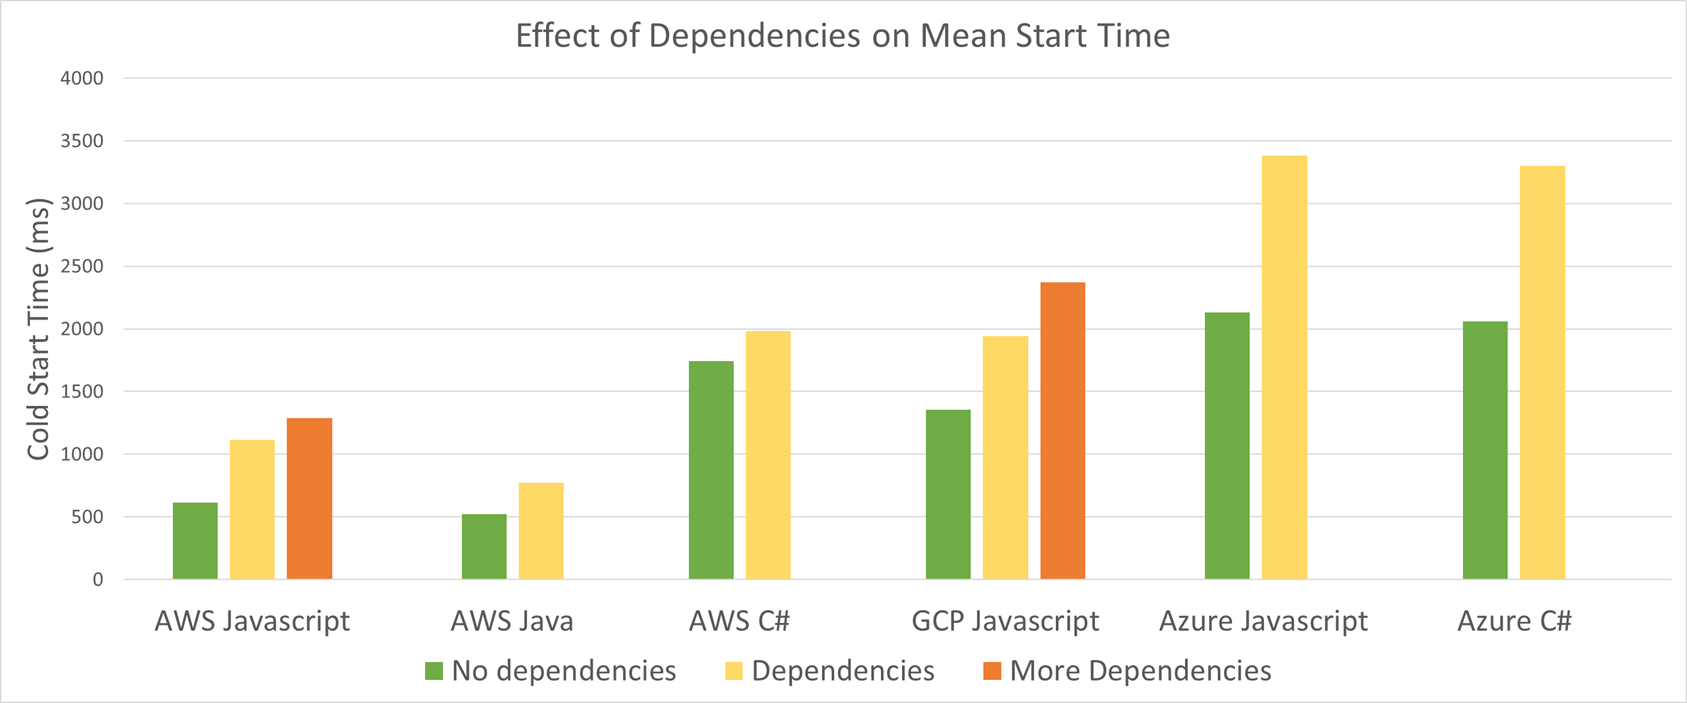
\includegraphics[width=80mm]{./thesis_images/cold_start.png}
    \label{fig:cold_strt}
\end{figure}

A solution for this problem, other than keeping the dependencies small, is to
have a warm function up at all times so it can handle the request right away for
time sensitive applications. The problem here though is that most commercial
offerings do not offer this option. Instead the developers are forced to keep
pinging the function to keep it warm for the next trigger. This is a very hacky
solution and reduces the whole efficiency of the platform in general. Most of
the cloud providers are although aware of this problem and are trying to be
innovative and introduce lighter alternatives to Linux containers in the FaaS
platform these days.

\paragraph{Parallelism}
\label{sec:org210d059}
Current FaaS offerings are not known to have the right support for heavily
parallel computations. In the most popular commercial platforms, the presence of
cold starts delays some invocations and increases the runtime. This impedes the
parallelism. In case of multiple
simultaneous requests, maximum parallelism that was achieved in handling them on
average was less than 50\% \hyperref[ref:17]{[17}] in Google Cloud Functions. The reason for
this can be further elaborated as follows:
\begin{itemize}
\item Virtualization technology: If a FaaS system has to run multiple functions in
parallel when triggered, the most import thing that comes up is the ability of
the platform to boot up more instances of the function instantaneously. The
quickness of the creation of the instances depends on the virtualization
technology that is being used. This is basically the cold start latency that
is affecting the parallelization. For example, if Docker is used as the
virtualization technology the system is seen to have a bit more latency, but
if a virtual machine is used the latency goes up exponentially. This calls for
the need for more lightweight isolation solutions. AWS firecracker is a step
in this direction.
\item Reactive scheduling: In FaaS systems the kind of scheduling that happens is
extremely reactive. Reactive model s seen to be too slow to scale. Achieving
high levels of parallelism requires being able to provide resources rapidly.
So how the system deals with the incoming invocation is very important. It is
seen that the current event based triggers are less that optimal for such
applications. This calls for a proactive approach in dealing with invocations.
It could be a more push based approach as opposed to the former.
\end{itemize}
\paragraph{Security issues in a multi-tenant environment}
\label{sec:orgbc0a4d5}
Like was previously mentioned, the whole FaaS infrastructure offering is
economical for the cloud provider because they get to share their node pool
among all their standard customers making the resource cost for them very low.
The problem with this practice though is that this introduces safety issues for
the data that is executed in the machines. Linux containers are not
particularly secure as an isolation mechanism since they share a Kernel with the
host operating system. This means that any bug or back door introduced to the
Kernel get affected to all the containers as well exposing the customer data at
a very high risk. This is an issue that is actively being worked on by
companies. Till a while ago, the solution for this was to encapsulate the
containers in a light weight VM which unfortunately contributed to the heavy
cold start time. But recently the innovative new alternatives for Linux
containers are also aimed at to fix these issues.

\subparagraph{Function caches}
\label{sec:org463c834}
Along with the above mentioned issue with multi-tenancy across customers, a
similar issue can occur under the same customer who runs an application across
multiple of their client. The problem is that each function has an inaccessible
cache that get cleaned up at an arbitrary time hidden from the user. There is a
chance that somehow cache from the previous execution of the function somehow
lingered and the data from one client got leaked on to another or got corrupted
by the other. If the developers are not cautious enough while coding and usage
of variables, there is a high chance for data corruption and leakage on the platform.

\paragraph{Developer friendliness}
\label{sec:org333f33e}
In a recent survey \hyperref[ref:16]{[16}], developers were asked about the challenges they face when
using Serverless platforms. This is a very significant data to look into since
at the end of the day the gap of the research and the end user experience is
something we are trying to mitigate with this project. The following were some
key takeaways from the study.
\begin{itemize}
\item Debugging and testing: Even though FaaS setup modularizes the code a lot, when
we consider most commercial offerings of FaaS, there is low to zero
possibility to actually follow the conventional testing and debugging
methodology. It is mostly because of the fact that the runtime of the FaaS
environment is not known to the developer at the time of the development.
Along with this, by the sheer nature of FaaS, it is often hard to mock exactly
the events like would in the production setup locally. So a full functional
testing of the platform is often pretty difficult to make happen.

More than often the developers have to depend on deployed setup of the FaaS
function and try debugging on production. This costs resources and on issues
involves re-deploying it and testing again. This has a huge impact on the
productivity and slows down the whole development workflow.
\item Logging and monitoring: Most of the current commercial platforms asks the
developer to user an external tool like AWS cloudwatch which costs more for
this service. Considering logging is the only way to debug the function, it
becomes a bit of an inconvenience if the developer is expected to pay for it.
As for the monitoring the same story applies. For each metric that is being
tracked extra is expected to be paid. If one is composing the functions, it
gets even more difficult to understand the cumulated runtime monitoring along
with the transfer details on the block storage, if any.
\item Standardizing development practices
The problem basically boils down to this one tag. The idea is that each of the
FaaS operator has a different kind of interface or way of dealing with the
events hence introducing a lack of standard dev practices. The problems are
more so prevalent when it comes to the building and deployment of the function
since the user management and the CLI access to do deployment are all
delegated to external tools.
\end{itemize}
\subsection{Extract-Transform-Load(ETL) pipelines}
\label{sec:orga57ddd5}
In the previous sections, we talked about how serverless is the most suited but
inefficient(with the current state of art) tool for ETL pipelines and that it is a
standard practice when dealing with today's data driven workloads. In this
section, we look in detail into the characteristics of ETL workloads and their applications.

ETL is the type of data integration process that is used to process data from
multiple sources to build a Data Warehouse or similar sinks. It integrates three
distinct but interrelated steps namely Extract, Transform and Load.

The main advantage of having ETL pipelines in the splitting of functionalities
in the data processing programs that would have otherwise been a single huge
monolith - hard to manage and extremely bloated.

\paragraph{Extract}
\label{sec:org5bbd83c}
In the present day production workloads, data can be arriving from numerous
sources of very varied nature and behavior. Depending on their origin source,
this data can have different formats or organizational structure. Some examples
for this are relational databases, XML, JSON, flat text files, etc. To allow
scalability in a software solution it is always necessary to have the tool
working for multitude of data types. This is where having a dedicated extract
process shine. Extract process accepts data from any of the data source and
format it to a unified data type. In general, in extraction phase developers try
to convert the data into a single format that is understandable by the
transformation phase. Another import thing the extract step take care of is the
validation of the data. The data that is coming from the source can be of the
wrong format as expected, even missing some columns or corrupted somehow. In the
extract step, these bad data are reported and the process is aborted.
\paragraph{Transform}
\label{sec:orgfa8ab36}
This step can be considered as the brain of the whole workflow. This is the
stage where we convert the data that was received into meaningful information.
Transform operation often happen in multiple stages where in each stage a
certain transformation logic is applied to the data. These logic can be simple
text formatting steps like splitting the data, cleaning the data, deduplication,
replacing codewords with meaningful entities etc. or more complex arithmetic or
logic operations like machine learning models. This step often ends up being the
bottleneck in a lot of ETL pipelines since data processing can be a very
resource heavy task and if the code is written with no optimization, the whole
pipeline will end up eating up the all the resources.
\paragraph{Load}
\label{sec:orge48cb99}
Like the name suggests this is the step where the data coming after the
extraction and transformation processed get loaded into the target data store.
This is a rather interesting process because the nature of the target store and
the communication API need to be analyzed efficiently to write the code. The
code often contains certain validation parameters to see if the current data is
suitable for insertion into the target. Common problems that occur might be
format difference from the target, duplication of primary or foreign keys, other
integrity violation issues, etc. Monitoring is critical in this step since there
is a chance that the target endpoint can go unavailable and the developers have
to make sure the data after the entire processing is not lost. More than often
the data output overwrites the existing data in the source, in other cases the
new data gets appended to the older ones or aggregated with the existing data.

\subsubsection{How Serverless can make a difference in ETL}
\label{sec:orgb76abf2}
Let us now look at some of the characteristics of the ETL processes that can be
derived from the definition.
\begin{itemize}
\item Atomicity of functions: In the pipeline, if a failure occurs in any of the above stage, it should stop
from proceeding to the next stage for that data without disrupting the
pipeline that is dealing with any other batch of data.
\item Each stage can have different loads depending on the operations and these
stages should be able to independently scale without scaling the other stages.
This helps in saving resources. Along with that it also saves from making any
one step a bottleneck because of low resource availability by scaling the
resources up as per necessity.
\item Intermediate data transfer need to handled properly by the system. We need to
have temporary data between each of the processes stored temporarily. This is
to make sure that if one of the stages fails, the data the came out of the
previous step is still available which can be processed again after the
developer fixes the issue with the current stage. This means that at any stage
you can restart the system and the pipeline can continue without issues.
\item There should be proper monitoring support make sure that we can easily see
when the errors are happening in the system. Along with that, the performance
of the pipeline should be quantifiable. We should be able to tell which stage
in the whole pipeline uses more resources, etc. and the overall performance of
the ETL workload.
\end{itemize}

It is clear from the above description why Serverless might be a good fit for
ETLs considering its elastic architecture and functional style of coding. Each
stage in ETL can be separate functions than can be independently scaled and
monitored. Although the aforementioned issues with the Serverless makes the
function composition and data transfer quite inefficient making it an ill suited
candidate for ETL applications. Also in the current Serverless solutions, it is
hard to achieve the atomicity of functions.

\subsection{Problem statement}
\label{sec:org103f384}
From the above set of evaluations, there is no doubt that Serverless Computing is a
solution with great potential as a tool for deployment and infrastructure provisioning. Even with the current
state of art FaaS offerings, 21\% of the entire workload is Data processing
applications that include heavy batch and streaming Extract, Transform and Load
operations \hyperref[ref:16]{[16}]. However, the implementation usually involves
numerous hacks in this setup, even after which the latency of the I/O, network
and the platform itself slows from leveraging the full potential of the idea.
All the existing commercial offerings being closed source and vendor locked in,
implies that the limitations are set for you by
the cloud provider and is often very difficult to fiddle with it or to extend
the system so as to support an extra runtime, increase the running time, etc.
Along with this, the way current FaaS offerings deal with function compositions
and parallelism are extremely clumsy and almost always explicit. While this lets
the providers have a very generic way of dealing with the platform and holds to
the one way to code them all paradigm, the gateways often tend to be a
bottleneck. Also the data transfer between functions always depend on a storage
based off of Block IO which contribute to the latency immensely.

When we look at the academic research in and around this area, in the past
couple of years a handful of ideas has been thrown into introducing state in
serverless. A very interesting proposal was Cloudburst \hyperref[ref:2]{[2}] which
introduces a consistent cache storage between functions to store and retrieve
intermediate data in wire speed. Although the project succeeds in proposing a
very elastic system architecture that co-locates data alongside functions across
the cluster, it is seen that the system does not scale really well along with
the requirement making it a bad adaptation for streaming and big data workloads.
Alongside, it lacks provisioning to define branches or conditionals in the function
composition making it less flexible from the point of view of the orchestration.

A similar idea was SAND \hyperref[ref:3]{[3}], where a hierarchical message bus is used to allow
function composition and inter process calls. Other than being a closed source
project and pretty abandoned in the past couple of years, the resource
allocation is not tracked or controlled by the system breaking the per usage
billing notion of Serverless paradigm. The system also does not offer a
proper isolation mechanism.

The focus of the thesis is mostly to propose a solution for the aforementioned
issues. We are proposing a Open Source infrastructure, infrastructure that can
be maintained by the companies which can offer a multi-tenant and completely elastic
platform to deploy their data intensive and high throughput applications on.
By nature, these data intensive applications can be a composition of multiple
functions, that would pass along data between them. The setup would user
ephemeral in memory storage to keep intermediate data. This infrastructure
would comply perfectly with the notion of Serverless in the sense that, each
element in the system would be independently elastic and scalable. Function
composition based on conditionals and branching should be supported by the
system along with independent scaling of the functions based on the load, so
there would not be any bottlenecks. An easily adaptable programmable API is
required for defining this composition.

According to the aforementioned survey, the developer community is concerned
about the monitoring and debugging of the functions during the development stage
due to the lack of reproducability of the runtime. Our system should give a lot
more flexibility and traceability when it comes to the development process.
Along with that, we should aim at building a system that is easily adaptable and
stable enough for production workloads, and easily integratable with the common
development tools like Github, CI/CD pipelines etc.

\section{Proposed Solution}
\label{sec:org75db54c}

In this section we dig in deeper into the specifications of our proposal to
build a production ready FaaS infrastructure stack that is completely elastic
and not locked into any vendor. The idea is that, any party or enterprise should
be able to reproduce this stack easily and developers should be able to deploy their
application code from any git hosting service or command line to this platform
without worrying about the server management. The platform we build also should
be provider agnostic, in the sense that it should work with constant efficiency
on any cloud provider the user may choose. The developer should be able to
monitor the usage and performance of the application easily.

In the light of the above discussion we propose the following extensions to the
existing Serverless platforms:
\begin{itemize}
\item Provision to compose functions by defining a computational graph
\item Ephemeral in-memory storage to store intermediate data
\item Multi-tenancy support by separating function instances using namespaces
\item Fine grained tracing and monitoring of the functions and the compositions
\end{itemize}

To clarify how the above mentioned steps will help solve major limitations of
Serverless paradigm, we will have a platform agnostic look at how the above
steps change the current state of art FaaS systems. In the section 5, we will
get into platform specific study by implementing these suggestions on a flexible
open source FaaS solution for our proof of concept.

\subsection{Function composition}
\label{sec:org04c9ce5}

Big data processing is pretty inevitable as an application scenario. The nature of these
data can be very varied including streaming, semi-regular burst streams, etc.
making it a very good space to apply Serverless paradigm to, to save up
resources and have fine grained scaling of the resources based on requirement.
The aforementioned complexity in the application logic suggests that it make a
lot of sense to split the application into multiple functions and compose them
efficiently. If applied to the Serverless logic, this means that each function
can be scaled independently based on the load in that logic.

The above requirement exposes some issues that were discussed in the section
2.2.4 of FaaS. Function composition is not something that has been cleanly
supported by popular commercial FaaS offerings. The popular infrastructure today
do not have any information about the dependencies between multiple functions.
It is up to the developer to programatically call functions from each other
which are packaged and deployed separately. If there are any heavy data to be
transferred among these functions, which we can refer to as intermediate
data, the developers are expected to use a block storage of some sort(eg: S3,
google data store, etc.) adding heavily to the Input/Output latency of the
service, not to mention the network latency if the infrastructure is in a
different VPC.

In a recent case study \hyperref[ref:18]{[18}], Autodesk claims their FaaS-ification of
their whole platform. Unfortunately, their account creation platform, which was
implemented as a composition of multiple small functions on AWS lambda incurred
a round trip time of 10 minutes. This is horrendous especially considering the
vitality of the task in discussion. Overhead of Lambda in task management and
the state management is explained as the causes.

More products has been introduced by cloud providers, like AWS step functions \hyperref[ref:19]{[19}]
, instead of fixing the inherent architecture of FaaS
solutions to help create data intensive workflows in FaaS. These systems work by
introducing an event queue like AWS SQS to the equation. The problem with such
solutions is that they violate the notion of Serverless in a way by introducing
an element that is practically non scalable and cannot be debugged easily. It
becomes extremely difficult to develop and test the system locally. Not
the mention, the fact that this introduces more lock in to the vendor.

Another approach can be found here \hyperref[ref:20]{[20}], where the function composition is
done by triggering the other functions by pushing intermediate data to s3, which
the following function considers as the trigger. The example in question is a
very simple map reduce which is not very intensive computationally even with a
heavy load of data. Even with that the setup takes around 2 minutes to complete
the task for a dataset of size 25GB. It can be seen that the majority of the
running time was spent on pushing and pulling data and not on the compute.

It is quite clear that the ability of functions to call each other are rather
important. There should be a way to define programatically the relationship
between the functions in a FaaS infrastructure along with the data flow
dependencies. If cloud provider exposes an API that would let the developer feed
a computational graph for this function composition, this would not just
improve the performance, but also would be useful for better function and data
placement so the latency for data and control transfer would be minimum. This
can be a very tricky thing conceptually since, containers are not directly
addressable network wise.

Before getting into the technicalities of the platform itself, let us look at
different approaches in which functions can be composed in a serverless
workload.

\subsubsection{Manual Compilation}
\label{sec:orgc7dd2ec}

This the most basic and inefficient way of compiling the functions. This
basically involves merging all the functions together to form a huge function.
From FaaS executor's point of view, it is one big function.

\begin{figure}
\caption{Merged in the source code}
\centering
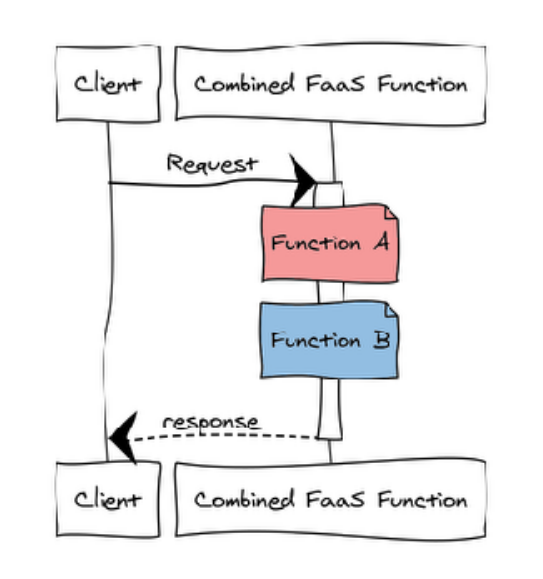
\includegraphics[width=80mm]{./thesis_images/manual_comp.png}
\label{fig:manual_comp}
\end{figure}

\begin{lstlisting}
def funcA():
  doStuff()

def funcB():
  doStuff()

def main():
  funcA()
  funcB()
\end{lstlisting}

The above code block and Figure \ref{fig:manual_comp} explains how the control flow works in this
kind of compilation scheme. As is pretty obvious, with this method one cannot
scale individual functions independently and function can get really big. There
is no necessity to store intermediate data or serialize and deserialize data
between functions. But the problem is that this kind of violates the notion of
serverless since each application is not an atomic functional unit. If the
compute is complex, function might not even completely run because of the
hardbound limit to the running time set on most FaaS platforms.

\subsubsection{Direct function chaining}
\label{sec:org23ae879}

\begin{figure}
\caption{Direct function chaining}
\centering
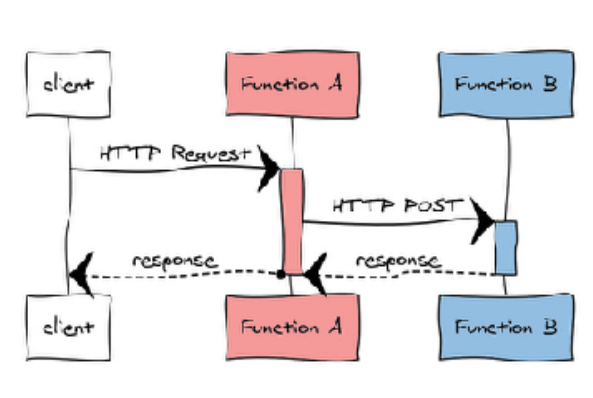
\includegraphics[width=90mm]{./thesis_images/func_chain.png}
\label{fig:Chaining}
\end{figure}

Like can be seen from Figure \ref{fig:Chaining}, here each task is a separate function. Each
function directly call the succeeding function in a chain. Meaning the code is
written so that the current knows the details of the next function, but not any
further. Even here like before, there is no need for any serialization
deserialization overhead since functions can directly send each other data. No
external components are used either. Although the problem arises when the data
load increases. The load on the network to transfer data via HTTP rises. Along
with that each function will have to wait for the next function. If a function
fails then the logic to retry/fallback etc. will have to be coded into each
function. The following pseudo code shows how the function design would be.


\begin{lstlisting}
def funcA():
  doStuff()
\end{lstlisting}


\begin{lstlisting}
def funcB():
  doStuff()
\end{lstlisting}

\subsubsection{Composition via coordinator functions}
\label{sec:org830f39f}

In this method, a coordinator function will be used which manage the execution
of all the functions by calling them directly. The individual functions will be
unaware of each other.

\begin{figure}
\caption{Coordination functions}
\centering
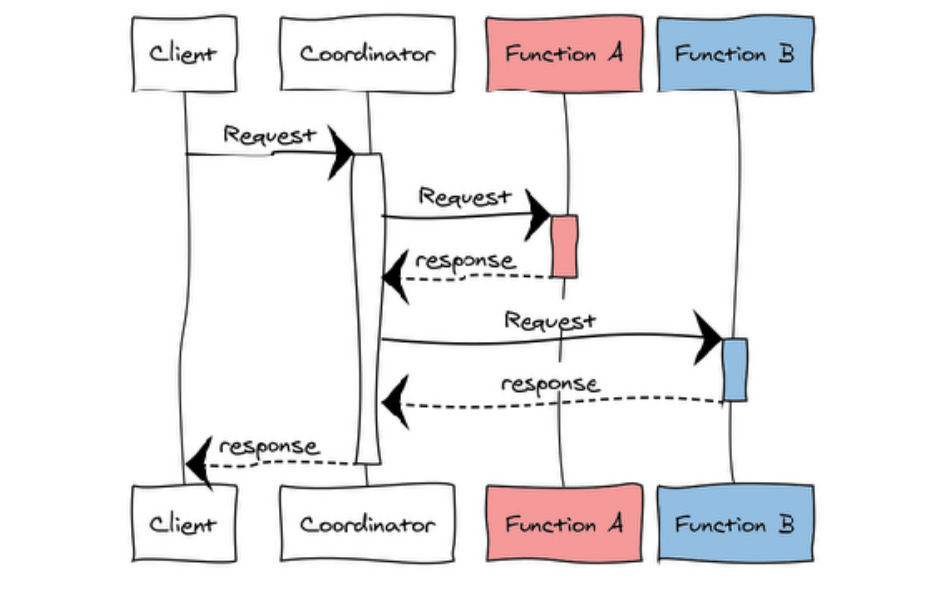
\includegraphics[width=150mm]{./thesis_images/coordination.png}
\label{fig:Coordination}
\end{figure}

The win over the previous method here is that, the house keeping code need not
be present in each individual task. Also it is very flexible in the sense that,
each function can be tested independently and then the user can properly write
the control flow in one place, that being the coordinator function. This comes
at a cost of adding an extra function which is the coordinator function. This
function will continue running the whole time, costing more and violating the
FaaS paradigm a bit. An example of this kind of coordination can be found here \hyperref[ref:21]{[21}].


\subsubsection{Event driven composition}
\label{sec:org34faabd}

\begin{figure}
\caption{Event driven function composition}
\centering
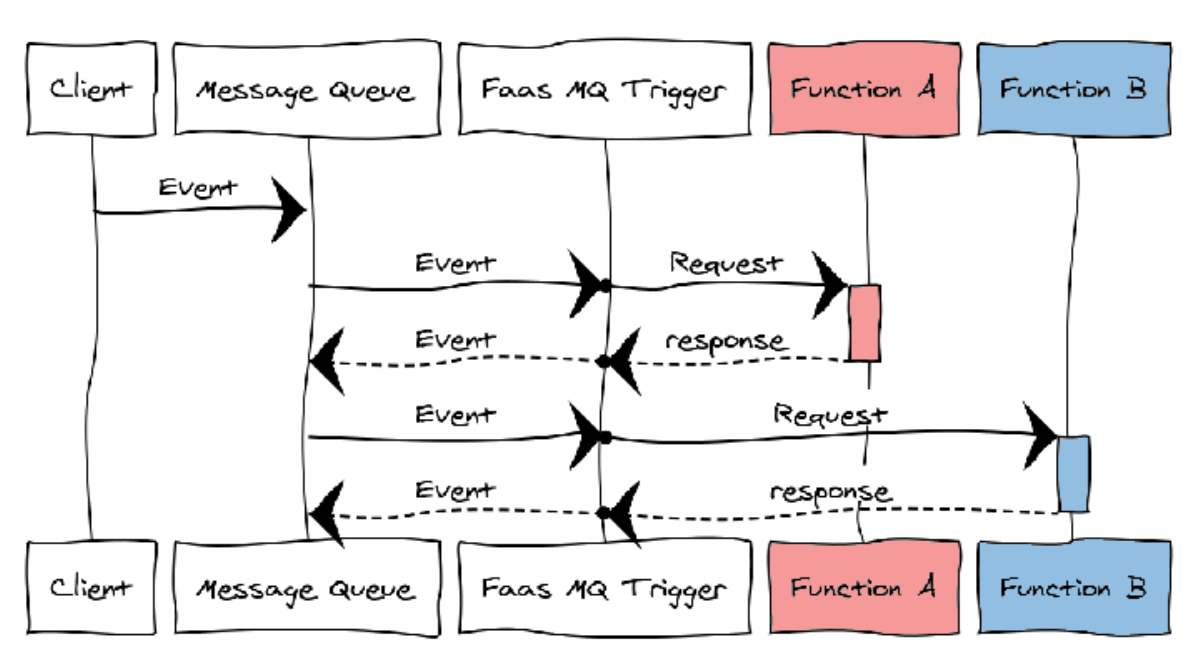
\includegraphics[width=150mm]{./thesis_images/event.png}
\label{fig:Event}
\end{figure}

This is a powerful design pattern that supports a lot more fault tolerance and
involves changing or extending the infrastructure of the FaaS platform. In this
method, one introduces message queues in the architecture as can be referred
from Figure \ref{fig:Event}. Functions emit events to these message queues. Alongside, all the
functions listen to the same queues. So on receiving certain events, they react
in the programmed ways. Contrary to all the previous methods, it is very
interesting to note that in this method, the stress is given to the data flow
instead of the control flow among functions. The intermediate data between the
functions has to be managed separately by using a storage.

This is a very commonly used and popular architecture. Message queues like Kafka
or MQTT brokers like rabitMQ offer a lot of functionalities and features like
fault tolerance, error handling, alerting, backup, etc. Functions can be
completely decoupled. This is a very good solution for big data and streaming
data applications.

The problem with this method is though the very heavy dependencies which are
very hard to manage. The fact that message queues are not inherently serverless
makes the platform less elastic and thereby billing and usage tracking can be
troublesome of the infrastructure manager. Alongside, message queues usually
only supports limited control flow structures. Probably just conditional and
on-error handles. It will be terribly complicated to do dynamic branching,
iterations, etc. Along with this, since functions are so tightly dependent on
the message queues, it will be slightly challenging to upgrade or version them.

\subsubsection{Workflows}
\label{sec:org6f90e98}

Workflows are a very interesting architectures pattern where the system supports
the creation of a sort of flowchart of the functional interaction. Workflows are
a very widely used pattern these days in a lot of big data processing tools.

An workflow is designed as a directed acyclic graph (DAG). This means that a new
runtime has to be introduced in the FaaS system to manage the execution of the
functions. When authoring a workflow, one should think how it could be divided
into tasks which can be executed independently. The workflow runtime would let
one to merge these tasks into a logical whole by combining them into a graph.

This definitely adds the overhead of writing a runtime for the FaaS platform,
providing an API to define the DAG to the runtime and then managing and
executing the workflow based on the DAGs. But once the platform is in place, it
provides numerous flexibility. One can get done dynamic branching, iteration,
etc. very easily on this platform along with individual upgrade of the
functions. The fact that no external infrastructure tool has to be managed to
work as a triggering mechanism maintains the elastic nature of the tool. The
only thing is that there has to be a storage unit to manage the state of the DAG
for the workflow framework. Similarly just the event driven composition, the
intermediate data store has to be handled separately.

Logically, this method resembles the coordinate function setup, just that
instead of a simple coordinator function, in this case we have a month more
powerful framework that is added permanently to the infrastructure. This can be
referred from Figure \ref{fig:Workflows}.

\begin{figure}
\caption{Workflows}
\centering
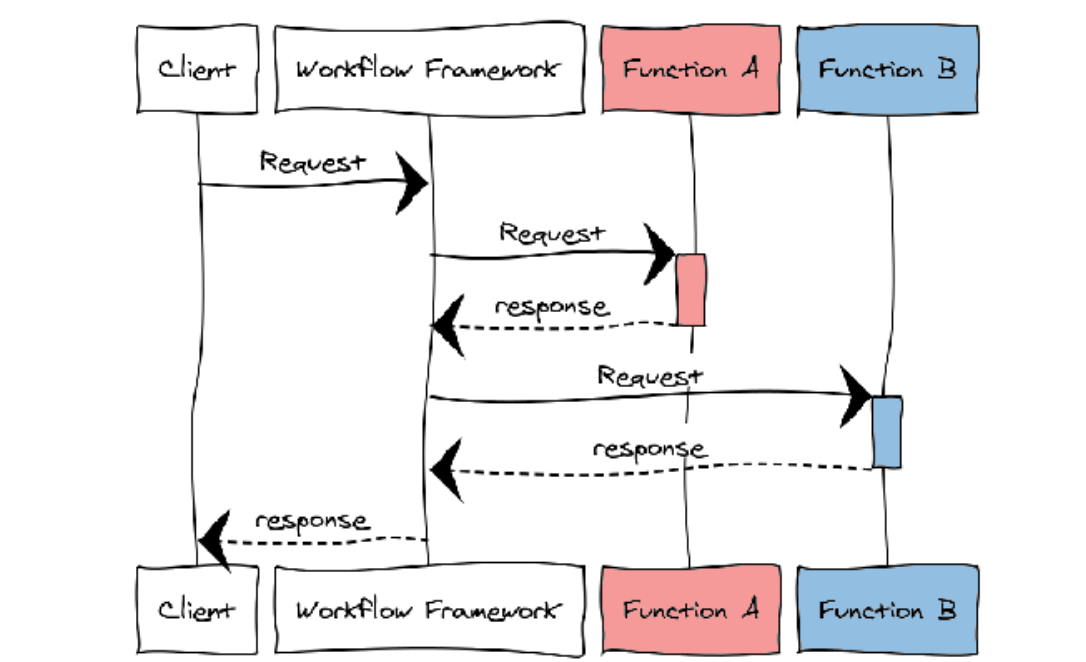
\includegraphics[width=150mm]{./thesis_images/workflow_2.png}
\label{fig:Workflows}
\end{figure}

The shape of the graph decides the overall logic of the workflow. A DAG can
include multiple branches and you can decide which of them to follow and which
to skip at the time of workflow execution. This creates a very resilient design,
because each task can be retried multiple times if an error occurs. To give the
reader clarity on what a DAG looks like, the Figure \ref{fig:DAG} from the Airflow's
operator might shed some light.

\begin{figure}
\caption{Branching example with DAGs}
\centering
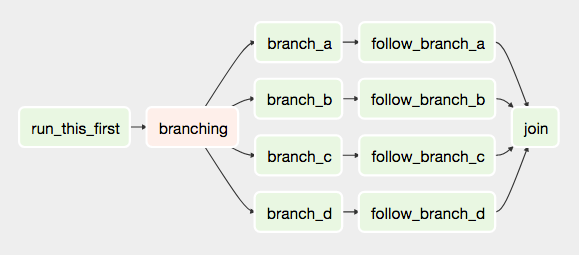
\includegraphics[width=80mm]{./thesis_images/workflow_1.png}
\label{fig:DAG}
\end{figure}

With this setup, we can get a lot more centralization to the compositional
logic, making logging and visualization lot more easier. With this method the
function scheduling and placement can also be improved. Meaning, functions that
have compositions with each other can be scheduled in the same node, if we have
a cluster or the intermediate data can be placed nearer, etc. One downside to
this method is that the user will have to use the workflow specific language or
DSL and not just the programming language used for the function implementation.


It is arguably clear that workflows offer the most flexible and application
independent solution as a composition pattern. Of course the concern of having a
storage for the running state of the workflow framework remains along with the
storage of the intermediate data. We will look into the solution to this in
section 4.2.


\subsection{Ephemeral Storage}
\label{sec:org506a975}

In the previous section, we saw that flexible function composition can be
achieved via workflow pattern. However, efficient state storage is necessary to make this efficient.
The problem is that we have to not violate the notion of elasticity
when it comes to Serverless. The resources involved in Serverless should be
scalable up and down, only when we can have a per usage payment and resource
conservation. Scaling up also affects the availability of the tool since one
should be able to have all the requested served without much latency. Along with
storing the state of the workflow or DAG, if function has to pass around data
from one function to another, we should introduce some sort of intermediate
storage since there is no direct communication between functions. The workflow
framework take care of triggering each function based on its state and the data
transferred between the functions will be via this intermediate storage as well.

In traditional analytics framework, long running process in nodes takes care of
managing the intermediate data in local storages. On contrary to this
conventional approach, Serverless workloads do not have any long running
processes. Because of the network addressing problem of containers, direct
transfer of data is also pretty impossible between functions.

In all the commercial service offerings of FaaS this intermediate storage is
done via a block storage like S3. This is a very inefficient approach since a
block storage adds a lot of I/O latency to the system. Along with that, it adds
a non scalable entity to the equation. Conventional storage systems are not
designed to meet the demands of serverless applications in terms of elasticity,
performance, and cost. We are talking about data that has limited life span,
which we can refer to as ephemeral data \hyperref[ref:22]{[22}].

Traditional storages like RDBMS, NoSQL, block storage, etc. are not made for
short lived data because of the latency involved in writing to the disk. An
in-memory key value store seem like the most obvious choice. But unfortunately
the industry standard key value stores like Redis does not scale very easily. One
has to take care of the scale of the storage cluster, network configuration,
maintenance, etc. Per use billing can also be very tricky in this case.

We should be looking into innovative new ideas to use for serverless platforms when
it comes to data storage because of the ephemeral and scalable nature of it.
Since Serverless functions are deployed on clusters that exist across multiple
nodes, a distributed key value cache that is scalable is the desirable option we
are looking for.

In our preferred storage medium, we should have automatic scaling, fine grained
usage tracking \& billing, low latency, high throughput, low cost, and unlimited
availability. Key value stores like Redis and memcache offer low latency and
high throughput but at the higher cost of DRAM. They also require users to
manage their own storage instances and manually scale resources \hyperref[ref:22]{[22}]. We look into
two different storage solutions for the adaption to our FaaS extension: Pocket and Orlic

\subsubsection{Pocket}
\label{sec:org6cb6a78}
Pocket \hyperref[ref:22]{[22}] is an ephemeral storage build for the Serverless workflows.
It is a key value store suited for storing and exchanging data between hundreds
of fine-grained, short-lived tasks. Pocket is an elastic distributed storage
service for ephemeral data that automatically and dynamically  right sizes
storage cluster resource allocations to provide high I/O performance while
minimizing cost. Pocket is not completely an in-memory storage
infrastructure like expected. Instead, pocket has a smart data allocation system
that leverages different storage media(DRAM, Flash, Disk) to store the data
depending on the requirement of the application while minimizing the cost.

Pocket has a tiered architecture. It has three planes - A control plane, a meta
data plane and the data plane. Like the name suggests data plane stores the data
ultimately. Meta data plane tracks the presence of the data distributed across
this data plane. Finally the control plane manages cluster scaling and data
placement. This layer keeps the platform elastic, in that it scales the storage
resources based on the usage. Each of the aforementioned layers can scale
independently. The project claims to have a sub-millisecond latency for I/O
operations.

\begin{figure}[!h]
    \caption{Pocket system architecture}
    \centering
    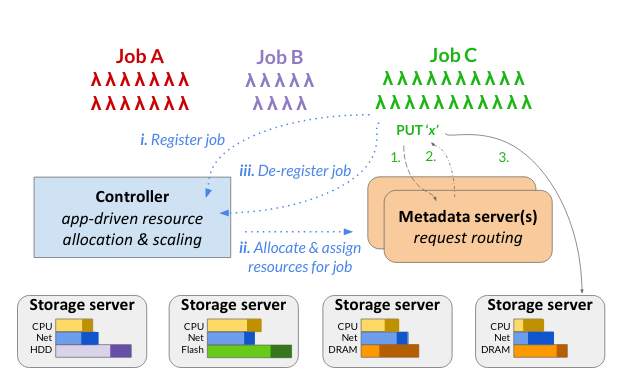
\includegraphics[width=80mm]{./thesis_images/pocket_arch.png}
    \label{fig:pocket}
\end{figure}

\subparagraph{Architecture}
\label{sec:org2ec5708}
Like Figure \ref{fig:pocket} represents, Pocket system has one centralized controller server,
one or more meta data servers, and multiple data plane storage servers. The
meta data plane according to us is the most interesting in the architecture,
since it enforces coarse-grain data placement policies generated by the
controller. It manages data at the granularity of blocks whose size is
configurable, defaulted to 64KB. Objects larger than this size is divided into
blocks and are distributed across storage servers by the meta data server. Client
access data blocks directly from storage servers.

\begin{figure}[!h]
    \caption{Pocket Client API}
    \centering
    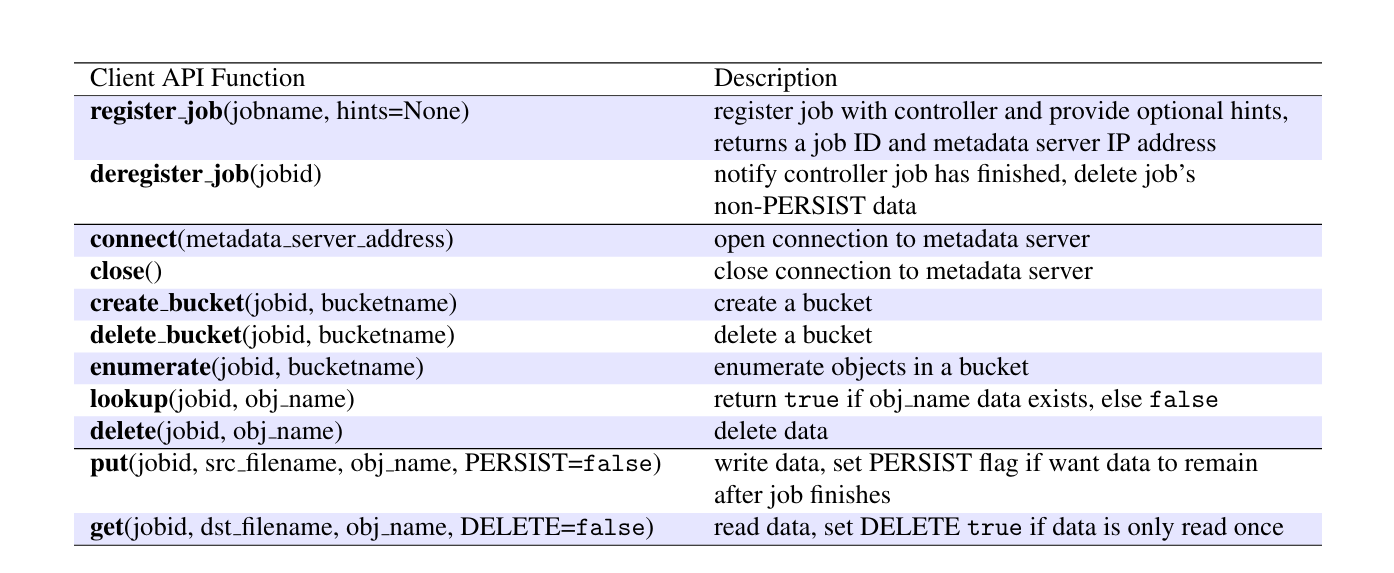
\includegraphics[width=180mm]{./thesis_images/pocket_client_api.png}
    \label{fig:pocket_api_client}
\end{figure}

\subparagraph{Client API}
\label{sec:org2afc632}
Pocket provides an API to communicate with the system. There are system calls to
each of the three planes. First of all it lets the client register and un-register of the
jobs(control plane). The client gets to communicate with the meta data server
multiple times during its lifetime. The data in pocket is stored as objects that
goes in buckets. They are identified using names. Meta data plane provides
system calls to create and delete these buckets, look up objects and delete
these objects.

Client put and get data directly to/from the object at a byte granularity. The
put and get operations invoke the meta data layer with the Job ID of the client.
This is to do the meta data look up operation to get the data placement of the
object that is being looked up. When a put call is invoked, with a PERSIST flag
to be true, the object will remain in the data even after the job terminates
despite the ephemeral nature of the storage. It will remain until it is
explicitly deleted or after a configurable timeout period. The get call with a
DELETE flag set will get deleted right away after returning the value of the
object. The nature of the ephemeral storage in discussion is assumed to be write
and read once only. Figure \ref{fig:pocket_api_client}, describes the system calls in detail.

\subparagraph{Implementation}
\label{sec:org4f1c820}
\begin{enumerate}
\item Controller:
\label{sec:orga232928}
Pocket is run on Kubernetes with each layer as separate docker containers. A
resource monitoring daemon is run on each node in the cluster sending resource
utilization info to the controller. The controller right sizes the cluster by
launching new nodes and sending the info of the existing meta data servers to
it. The load is balanced using data steering new active job data to the newer
server than balancing out existing data since this can add a heavy overhead
especially since the data is short lived. The container also keeps the meta data
server resource usage under the target limit by precalculating the load a job
would  put on the meta data server from its throughput and capacity allocation.
Based on this estimate the controller select the meta data server.
\item Meta data and Storage tier:
\label{sec:org6179ed8}
These are implemented on top of Apache Crail distributed data store \hyperref[ref:23]{[23}].
Crail is designed for low latency, high throughput storage of arbitrarily sized
data with low durability requirements. Crail provides a unified namespace across
a set of heterogeneous storage resources distributed in a cluster. Its modular
architecture separates the data and meta data plane and supports pluggable
storage tier and RPC library implementations. As of the storage tier, Pocket
project implements it on DRAM, NVMe on top of ReFlex and then on generic block
storage.
\item Client library:
\label{sec:orgb18bfd2}
The API is written in Python to provide better adaptability of the tool. The
core library although is in C++
\end{enumerate}

\subparagraph{Analysis}
\label{sec:org7740872}
\begin{figure}[!h]
    \caption{Pocket Performance for get and put requests}
    \centering
    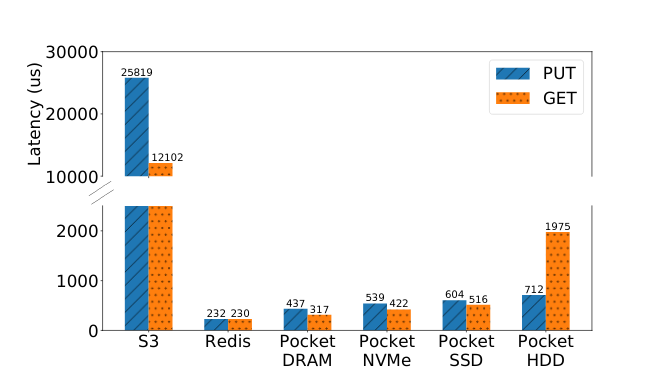
\includegraphics[width=100mm]{./thesis_images/pocket_perf.png}
    \label{fig:pocket_perf}
\end{figure}

Pocket is seen to have pretty good performance almost comparable to Redis but
much better economically when set up on DRAM. It is seen to be almost 300\%
faster than S3 storage for the GET requests. It can be seen from Figure \ref{fig:pocket_perf}.
So considering that DRAM will be used as the storage tier, it can be the
right tool for the ephemeral storage in Serverless platforms.

\subsubsection{Olric}
\label{sec:org27c8ded}
Olric \hyperref[ref:24]{[24}] is a distributed in-memory key/value data store. The idea is
that we can create a shared pool of RAM across a cluster of computers to store
the data in, in a scalable manner. The design motives for Olric is to share
between servers fast-changing transient data. At the time of writing, Olric
supports multiple serialization formats including JSON, MessagePack, etc. By
utilizing the heuristics of Kubernetes, Olric provides horizontal scalability to
the RAM pool available. Olric uses a consistent hashing algorithm \hyperref[ref:25]{[25}] to distribute
the load fairly among the cluster members. Olric best-effort consistency
guarantees without being a complete CP (indeed PA/EC) solution. This thread safe
in-memory cache comes with replica support and a command line interface.

The data is stored inside distributed maps which can be thought of as a bucket.
Inside each distributed map, there can be numerous key - value pairs. As for the
operations, currently Olric support atomic operations and the lookup
has a complexity of O(1). Olric uses SETNX algorithm to implement locking
primitives inspired from Redis protocol \hyperref[ref:26]{[26}]. Olric can be used either as a
Go library or as a language independent service.

The architecture of Olric is rather sophisticated. Olric distributes data among
partitions that are distributed across the cluster using the consistent hash algorithm. Every partition is being
owned by a cluster member and may have one or more backups for redundancy. When
a distributed map entry is being written, the communication is to the partition
owner. In a stable cluster, the query hits the most up-to-date version of that
data entry. In order to find the partition which the key belongs to, Olric
hashes the key and mod it with the number of partitions.

There is an elected coordinator in each cluster. The coordinator election is
done via a very simple heuristics. All the machines share their birthdate in the
cluster. The oldest machine gets elected as the coordinator. When the
coordinator leaves, the second oldest gets elected. It manages the partition table.
This can involve registering new partitions if a new machine joins, removes
outdated data, pushes new partition table to all the members and to the cluster.

There is a rebalancer binary running in each node that takes care of relocating
the partition from the backup to the new host when one of the hosts leaves.
Along with this it merges fragmented partitions.

The idea of fragmented partitions are rather curious. Each partition has an
owner. There can be multiple owners in which case the partition is called a
fragmented partition. The last added owner is called a primary owner. Write
operation is only done by the primary owner. The previous owners are only used
for read and delete. When you read a key, the primary owner tries to find the
key on itself, first. Then, queries the previous owners and backups,
respectively. The delete operation works the same way. The data(distributed map
objects) in the fragmented partition is moved slowly to the primary owner by the
rebalancer. Until the move is done, the data remains available on the previous
owners. The distributed map methods use this list to query data on the cluster.


\subsection{Multi-tenant security and isolation}
\label{sec:org189ad16}
A multi-tenant cluster is shared by multiple user and/or workloads which are
referred to as tenants \hyperref[ref:27]{[27}]. It is very crucial to make sure that data is
completely segregated between the tenants and in no circumstances can data of
one tenant be visible to the other. This is considered one of the biggest
security risks \hyperref[ref:28]{[28}] of the cloud multi-tenancy. Along with this it is
critical to make sure that the resource is distributed equally among the tenants
and in no way a starvation occur in the cluster. It is very important to keep in
mind the security implications of sharing certain kind of resources among
tenants.

In the case of FaaS, we already saw that how the same function instance can be
reused for different tenants and the cache can be lying around corrupting the
data or worse, exposing it. Along with this if there are functions that deal
with very sensitive information of a client, it is often very unsafe to schedule
other tenants' operations in the same node.

In this thesis, we leverage Kubernetes to guarantee isolation of data in a
multitenant setup. We separate each tenant and their resources into their own
namespace \hyperref[ref:29]{[29}]. Along with this we leverage policies \hyperref[ref:30]{[30}] by Kubernetes to enforce
resource limits to each client and manage access. By default, compute resources
on a Kubernetes cluster are unbound. With Policies we can set quotas or restrict
completely any or all kind of resources available to a pod. A LimitRange is a
policy to constrain resource allocations (to Pods or Containers) in a namespace.
A resource quota, defined by a ResourceQuota object, provides constraints that
limit aggregate resource consumption per namespace. Then we have Pod Security
Policies \hyperref[ref:31]{[31}]. This is used to make sure that each pod that runs comply by
certain security policies and permissions. This is what will be used in our
system to ensure that extremely sensitive pods will be scheduled separately
from the rest of the pods. Figure \ref{fig:multitenancy} shows how a multitenant
system looks like controlled by Kubernetes policies.

\begin{figure}[!h]
    \caption{Multi-tenant infrastructure}
    \centering
    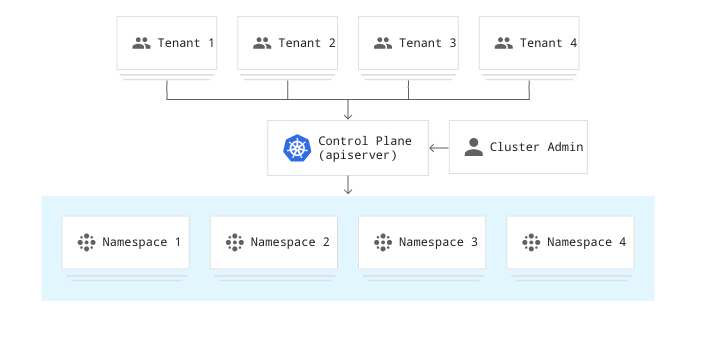
\includegraphics[width=130mm]{./thesis_images/multitenancy.png}
    \label{fig:multitenancy}
\end{figure}

\subsection{Monitoring and tracing}
\label{sec:org6c9856c}
According to a survey of 2018 done by Serverless(the company) \hyperref[ref:16]{[16}], the
second most thing the devs are worried about the development process of a FaaS
application is monitoring and logging. Monitoring, logging and tracing are all
ways to ensure correctness in your system. Monitoring serverless application is
very complex. In a traditional application, we usually focus on monitoring the
execution of code, while in serverless, we also need to monitor the integrations
between the different services and make sure that we can follow a request end to
end in our distributed system.

The demonstrate the issue a bit better, we consider a real AWS Lambda workload
and look at the logs \hyperref[ref:32]{[32}]. We deploy a function with a clear bug as a zip file with the
CLI of AWS. We get a HTTP endpoint for the function. This endpoint can be tried
hitting with an API client like postman to get a 200 OK result as seen in
Figure \ref{fig:postman}.
\begin{figure}[!h]
    \caption{Trying to hit the AWS Lambda function endpoint via REST API client}
    \centering
    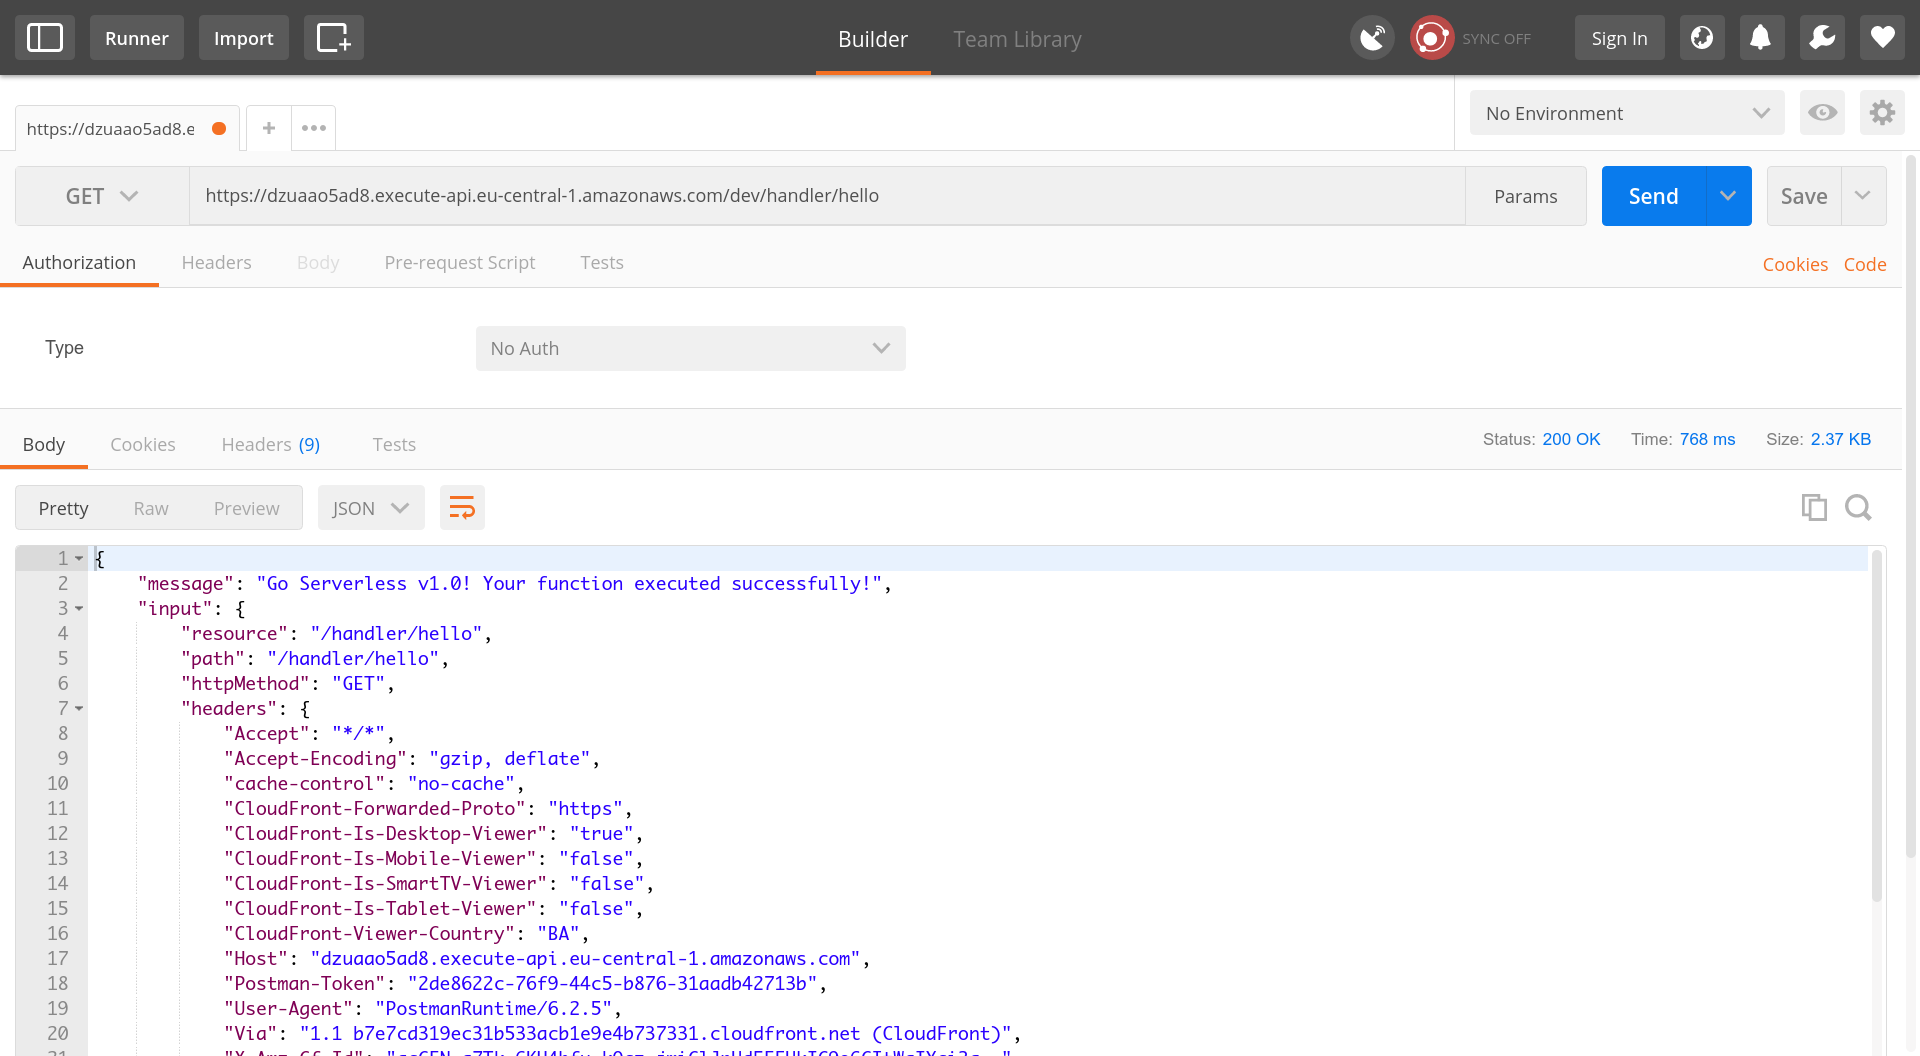
\includegraphics[width=100mm]{./thesis_images/postman.png}
    \label{fig:postman}
\end{figure}
\begin{figure}[!h]
    \caption{AWS Cloudwatch log of the same function}
    \centering
    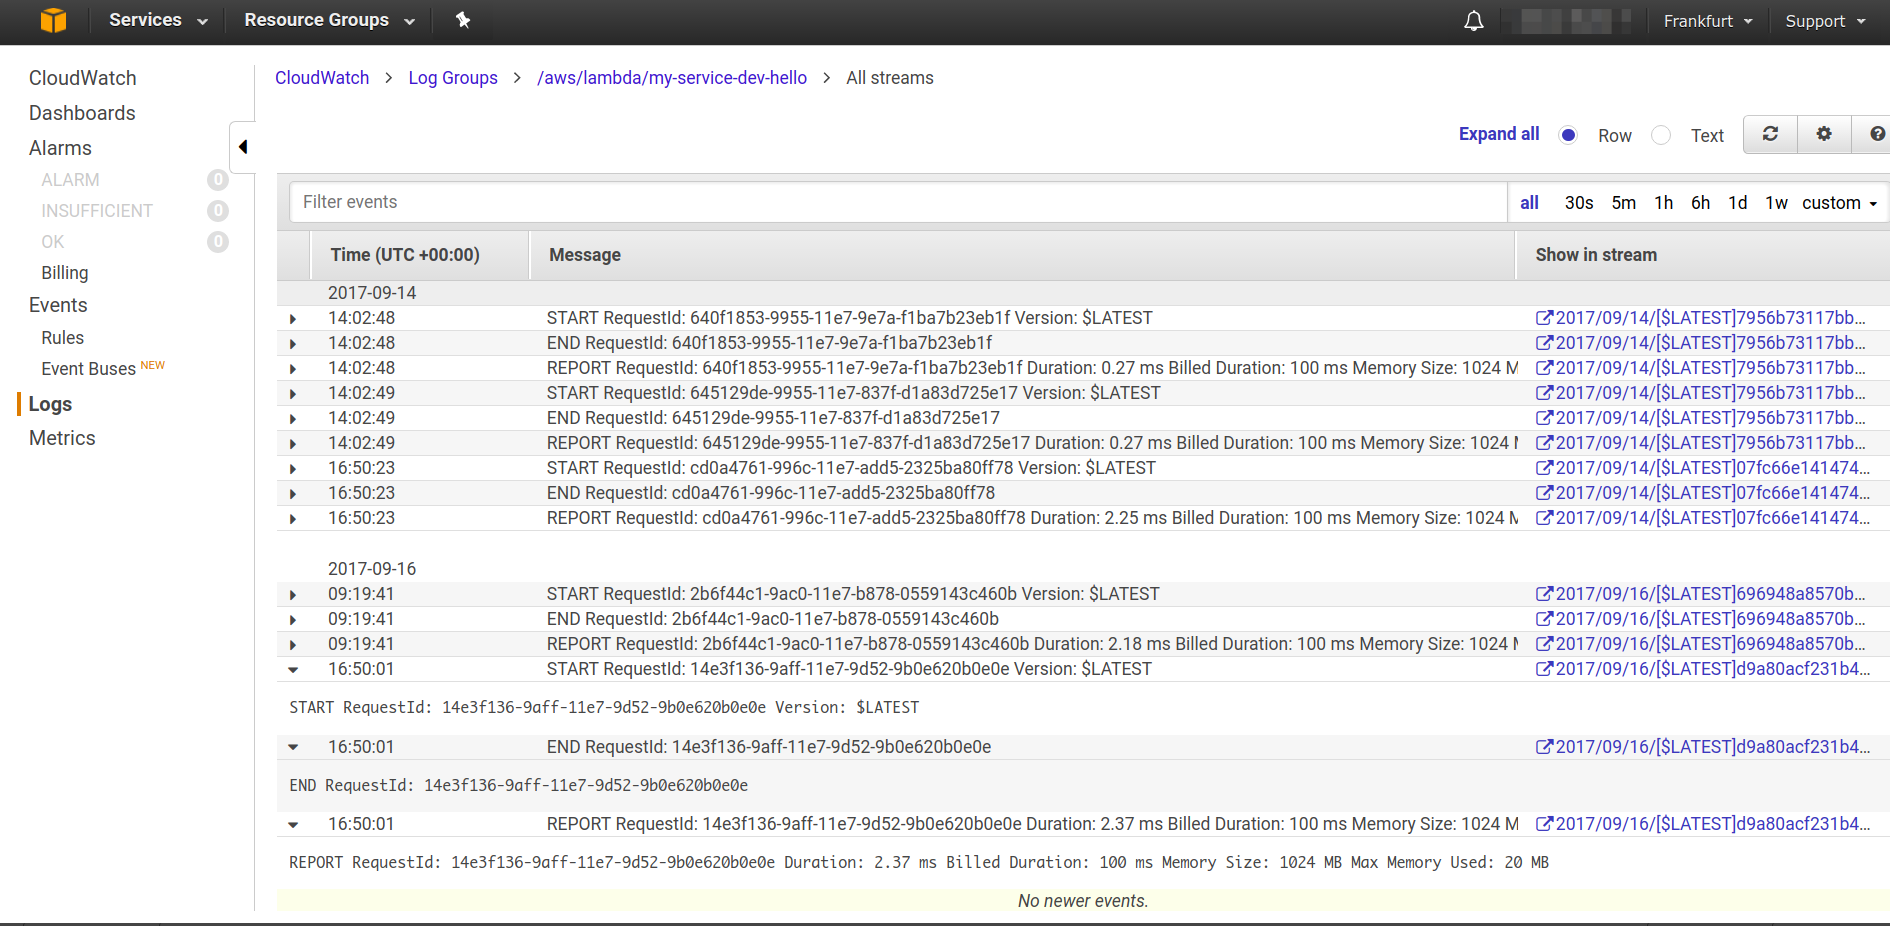
\includegraphics[width=100mm]{./thesis_images/cloudwatch.png}
    \label{fig:cloudwatch}
\end{figure}

AWS Lambda provides the logs via AWS Cloudwatch. We now look at the logs
produced by AWS Cloudwatch upon invocation. This can be found in Figure \ref{fig:cloudwatch}. As
you can see the logs are very fine grained, but the problem is that the logs
make no sense or helm the developer in the debugging process. Error messages for
failing functions are not verbose enough, so they often go unnoticed. We also are
having a hard time finding functions that timed out. This basically clears up
why we need more innovations in the monitoring of Serverless functions.

Let us understand first what monitoring, logging and tracing entails as functionalities.
\subsubsection{Logging}
\label{sec:orgfe9f48c}
Logging is used to track errors that were encountered in an app and other
debugging information of the running app. Even if the application is distributed
or otherwise, a good logging system will accumulate the logs and provide it in a
centralized way for the ease of the developer. Log files can show any discrete
event within an application or system, such as a failure, and error, or a state
transformation. When something inevitably goes wrong, such transformations in
state help indicate which change actually caused an error.

Since log files can grow exponentially, it is very important to analyze before
setting the logging framework in place what are the things that need logging. We
only need to know the crucial information but be mindful not to omit the ones
that might contribute to the debugging of the system. Even with this logging
system often tend to eat up all the storage in the systems. There are several
strategies that can be adopted to evict this problem. One way to deal with this
is to set a retention period to logs and clear up the log entries that are older
than this date. In most cases this would work really well since there is seldom
need for looking into significantly older logs. Another way to deal with bloated
logs is to rotate the log files. This is the practice where you write to a
different log file in a time window. This time window can be a day or a week or
a month and so on. The older log files are compressed and backed up someplace if
need arises to use them. The most recent logs will be available in the current
log files. This is a heavily adopted log handling mechanism.

A very good logging system will have a clean and standardized structure that
lets the developer read through it and debug easily. keep in mind that logging
should be precise and on point. It is also important to keep in mind whom is the
log for \hyperref[ref:33]{[33}].

\subsubsection{Tracing}
\label{sec:org10a4b24}
Traces are intentionally a noisier set of data that logs. When logs document
discrete events happening in the application, traces document a much wider
continuous control flow in the application. The idea is to track the data flow
and the control flow in the application completely. There is a lot more
information available in the traces as opposed to the logs.

The goal of tracing is not debugging but optimization. Traces often track the
whole lifecycle of one single request. This makes it easier for the developers
to understand the bottlenecks and other performance issues in the application.
It can often be used along with the logs when a problem occur. Traces can tell
you what has lead to that problem and how the previous functions have
contributed to the issue.

Traces need not be very reactive as opposed to the logs. Considering the amount
of data involved, it is easy to see that how resource intensive can tracing be.
It is often very hard to manage and it involves writing a lot more code to make
sure the framework catches everything we need to. But in microservice or FaaS
architectures, traces can be crucial since there are a lot of connected separate
parts involved in the pipeline and traces let you have a complete overview of
your workflow in action.

\subsubsection{Monitoring}
\label{sec:org21b3e1b}
Monitoring is a wider term that can be applied for both tracing and logging. But
in this context we talk about more complex monitoring systems. Monitoring here
helps the developer understand how their overall system works. It involves
instrumenting an application and then collecting, aggregating and analyzing the
metrics involved in the system. The main purpose of the monitoring system can be
considered as alerting the developers issues going on in the platform before the
users find out. These issues can be more system specific like out of memory, out
of storage, or other system failures.

There are various metrics from the system or the application that you can feed
to your monitoring platform. Recently systems developers have started feeding
application logs as well to monitoring platform so that they can get alerts as
soon as an error appears in the application log.

\subsubsection{Adaptation in FaaS}
\label{sec:org8cacbec}

\paragraph{Logs}
\label{sec:org021c6e5}
While working with an OpenSource FaaS platforms where the isolation is managed
by Docker, we can use the inbuilt logging system by Docker which are standard
systemd logs \hyperref[ref:34]{[34}]. We will not get into details of that here.

With the kind of distributed system that we have in our hands, in this thesis we
propose adapting distributed tracing to trace and monitor the
function instances.

\paragraph{Tracing}
\label{sec:org76a7935}
Distributed tracing is a method used to profile and monitor applications,
especially those built using a microservices architecture. Distributed tracing
helps pinpoint where failures occur and what causes poor performance \hyperref[ref:35]{[35}].
Opentracing \hyperref[ref:36]{[36}] is a standard specification for the definition of tracing
information. Systems that are written following this specification can be ported
from one tracing framework to another without having to change the
implementation. There are some fundamental attributes of Opentracing API that
are worth understanding. Refer Figure \ref{fig:traces}.
\begin{itemize}
\item Span
It represents the most atomic unit of logic in a pipeline. This unit will have
a name, a start time, and the duration
\item Trace
A trace is basically a collection of spans. It represents the workflow of the
entire pipeline. Each distributed component in the pipeline contribute their
own spans to form the trace from the aggregation.
\end{itemize}

\begin{figure}[!h]
    \caption{Spans and traces}
    \centering
    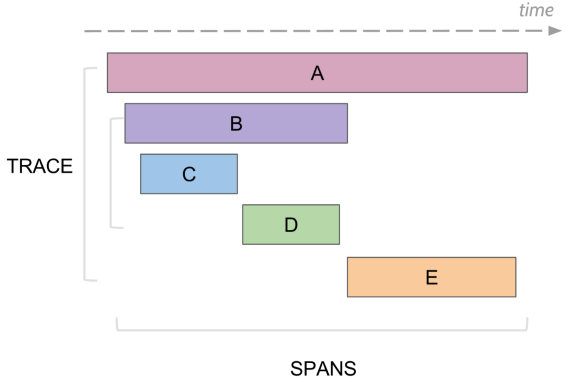
\includegraphics[width=100mm]{./thesis_images/traces.png}
    \label{fig:traces}
\end{figure}

As the definition goes from the documentation, OpenTracing is a way for services
to “describe and propagate distributed traces without knowledge of the
underlying OpenTracing implementation.”. The idea of tracing was well covered
before. What Opentracing adds to it is the capability to make tracing
infrastructure independent and standard across platforms. With the span and
trace form of specification, OpenTracing makes it easier to:
\begin{itemize}
\item Spans of services
\item Time taken by each service
\item Latency between the services
\item Hierarchy of services
\item Errors or exceptions during execution of each service.
\end{itemize}
\paragraph{Monitoring}
\label{sec:org3dd3fb3}
Monitoring of distributed systems can be heavily challenging but yet highly
necessary. The best industry recommended way is to do Time series monitoring
suggested by Google via the proprietary tool Borgman \hyperref[ref:37]{[37}]. It
is basically an in-memory database that scrape different kind of metric from
the system and applications. Then it does a rule based extraction from the data
and provides a queryable time-series database. Borgmon relies on a common data
exposition format; this enables mass data collection with low overheads and
avoids the costs of subprocess execution and network connection setup. The data
is used both for rendering charts and creating alerts, which are accomplished
using simple arithmetic. Because collection is no longer in a short-lived
process, the history of the collected data can be used for that alert
computation as well.

In our FaaS application, such a system basically can scrape the system
information from the Kubernetes cluster since each function is a pod. Then we
can specify appropriate rules for the kind of data aggregation we want to see,
visualize it and setup alerts. We will be using an Open Source alternative
which we discuss in the next section.


\section{Implementation}
\label{sec:orgf0e7773}
For implementing the aforementioned strategies and verifying its effectiveness
in making the Serverless workflows efficient, it is important to trial it on a

are closed in its source and vendor locked is practically impossible and
stalling the growth of Serverless as a paradigm. Instead several Open Source
FaaS infrastructure were analyzed for this thesis for the implementation of our
ideas. Along with the platform, choosing the right orchestration and clustering tools, the
workflow implementation tool, the right monitoring tools, etc. are also vital in
the implementation. So before going in detail about the architectural specifics
of the implementation, let us analyze the tools used in the process and the
reasoning behind their choosing.

\subsection{Tools}
\label{sec:org66d93b2}
\subsubsection{Container Orchestration}
\label{sec:orgefeb169}
We are going to work with a containerized setup like was hinted at the beginning
of the thesis description. Each function that is being written will be
containerized and brought up and down, scaled up and down based on the
configurations and usage requirement. We have to go with the right
containerization platform and an clustering tool that would take care of
managing, scheduling, scaling up and down, etc. of these containers across a
cluster of nodes agnostic of the application specifics or the underlying systems
specifics. We of course go with the industry standard here which are Docker and
Kubernetes especially because all of the leading FaaS solutions these days work
on both of these technologies. A gentle introduction to both tools before
proceeding to FaaS specific solutions.
\paragraph{Docker}
\label{sec:orga76d19c}
Docker \hyperref[ref:38]{[38}] is one of the leading Linux Containers solution that is being
adopted very widely across all kinds of software infrastructure maintenance
environments. According to the Docker Inc., over 3.5 million applications have
been placed in containers using Docker technology and over 37 billion
containerized apps have been downloads \hyperref[ref:39]{[39}]. Advantages of using
containers for application shipping was already seen in Section 2.1.2. Docker
made the whole Linux Containerization landscape a lot more approachable as a
packaging technology by the introduction of namespaces.

Without delving too much into the technicalities of containerization, we would
like to quickly explain the life of a containerized application with Docker.
Some terminologies that would help with understanding the concept:
\begin{itemize}
\item \textbf{Docker image}: Like in any virtual machine environment, images can be thought of somewhat a
snapshot of the current state of an execution environment(which is basically a
stripped down operating system with applications installed on it, ready to run).
What makes Docker images unique is its immutability. You cannot modify a docker
container. You can create copies or delete and recreate but not change the
state. This helps in guaranteeing that once your Docker image has reached a
working stage, it will always continue working no matter what. You can try an
add changing to the running instance of this image, but none of these changes
are persistent from the point of view of the image. You can shut it down and
start from the same image state as was created.

Sharing these images is an extremely easy process. There are container
registries which are hosting services for docker images like Github is for git
tracked code. Popular publicly available container registry is DockerHub \hyperref[ref:40]{[40}].
Developers can push their docker image to docker with a simple
`docker push` command from their command like and share or make it publicly
available for other developers or software tools.

To create a docker image, the most straightforward way is via a configuration
file called Dockerfile. According to the reference from \hyperref[ref:41]{[41}],

\begin{quote}


"Docker can build images automatically by reading the instructions from a
Dockerfile. A Dockerfile is a text document that contains all the commands a
user could call on the command line to assemble an image. Using docker build
users can create an automated build that executes several command-line
instructions in succession."
\end{quote}

For example, the following code block shows a Dockerfile written to dockerize a
simple Python app, that runs a simple flask HTTP server.

\begin{lstlisting}
FROM python:3.6.1-alpine
WORKDIR /project
ADD . /project
RUN pip install -r requirements.txt
CMD ["python","app.py"]
\end{lstlisting}

\item \textbf{Docker Container}: If Docker image is a digital photograph, a docker container is like a printout
of the photograph \hyperref[ref:42]{[42}]. Containers can be thought of as a running instance
of the image. Each container is run separately and unlike the images, you can
change the running container. If you want to persist these changes though, you
will have to commit the running container it its running state by committing it
as a new image. Your host operating system isolated the running container from
the others in the computer. Each container instance will have its process
namespace, limits on the resource usage, allowed system calls, etc.
Communication across containers can be setup explicitly. Most production
applications, usually have multiple containers running together with
communication internally so as to isolate each process environment, to avoid
cascaded application damage, etc. A container is inherently not addressable
directly from external network, although one can open it up by exposing
corresponding service port to that of the host system, provided necessary
security precautions are taken.

\item \textbf{Orchestration tools}: Docker by default ship a couple of orchestration tools that are specific to
Docker. An significant one among this is a docker-compose. Docker-compose lets
one tie up multiple docker containers, expose certain ports in each docker
containers, pass environment variables, define the communication and storage
usage rules, etc with the help of a configuration file by default to be name
docker-compose.yml. This is a very simple tool to use that helps in most basic
usages of the application deployment. One can connect multiple nodes together
and deploy the containers across these nodes via docker-compose using a library
called docker-swarm. Docker swarm takes care of very basic scaling up and down
of containers etc.
\end{itemize}

\paragraph{Kubernetes}
\label{sec:org4ddf654}
Now that we have seen a popular containerization solution called Docker, it is
time to see the most popular orchestration solution. Docker swarm was already
mentioned but when it comes to modern applications, the requirement goes far
beyond this. The application needs better scaling heuristics, version rollout
policies, cluster management, better networking and application discoverability,
better monitoring and alerting systems, etc. This takes up to a much more
advanced container orchestration platform called Kubernetes. It is worth noting
that Kubernetes is not just built for Docker but for multiple flavors of Linux
Container technologies.

Kubernetes is an Open Source platform for managing containerized workloads and
services, that facilitates both declarative configuration and automation \hyperref[ref:43]{[43}].
Contrary to the traditional deployment setups where applications ran on physical
servers, we have moved to an era where we deploy packaged applications and are
deployed across clusters of virtual nodes provided by cloud providers. We
require smarter tools for this to manage complexities in different levels
starting from application packaging to cluster management. Kubernetes can be
considered as the most popular solution that deals with these complexities.

Kubernetes provides the framework to run these applications along with the tools
for the following purposes \hyperref[ref:43]{[43}]:
\begin{itemize}
\item Service discovery and load balancing
\item Storage orchestration
\item Automated rollouts and rollbacks
\item Automatic bin packing to make sure optimal resource usage
\item Secret and configuration management
\item Monitoring the usage and load to the cluster and applications
\end{itemize}

A great thing about Kubernetes as project these days, is the community support.
It has a very large and widely adopted community. Along with that most cloud
providers now support out of the box kubernetes engines making the development
of infrastructure agnostic applications very easy. This is the way to go to be
away from a deployment cycle that is not completely vendor locked in.

\begin{figure}[!h]
    \caption{Kubernetes infrastructure}
    \centering
    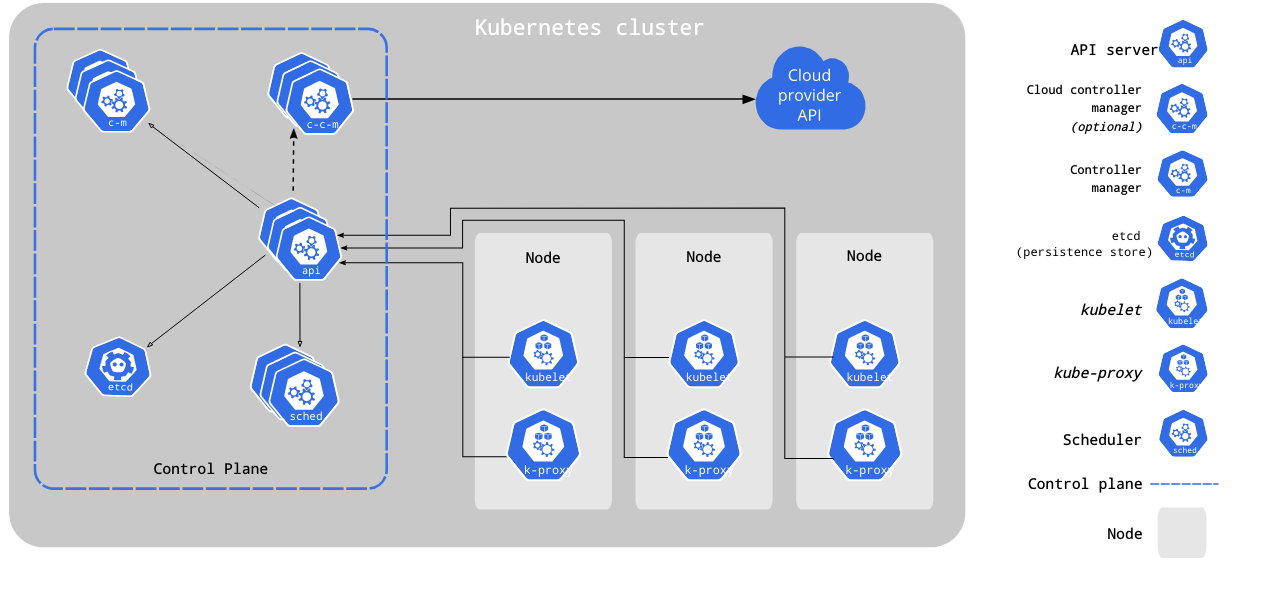
\includegraphics[width=180mm]{./thesis_images/k8s.png}
    \label{fig:k8s}
\end{figure}

Kubernetes is an immensely complex piece of software with numeral tools and
add-ons. Figure \ref{fig:k8s} depicts the architecture of Kubernetes. The control plane is
the core component of the setup. It consists of the API server to the platform,
etcd to store the state of the cluster, scheduler to deploy the Pods(collections
of containers that makes up an application) to the corresponding node in the
cluster evaluating the usage requirements and availability, cloud controller
manager that links the logic of the cluster to the API of the cloud provider,
etc. At the risk of getting out of this scope of the thesis, we do not analyze
more of the technicalities of kubernetes.

In our implementation, we will use the heuristics of scaling provided by
kubernetes in multiple cases. Alongside, the web UI kubernetes provides lets us
visualize the resource usage by the platform and applications to a great
extending helping with the monitoring of the setup.

\begin{itemize}
\item \textbf{Namespaces}: It is very useful to understand the concept of Namespaces in Kubernetes though.
We can logically divide each cluster into multiple virtual clusters called
namespaces. It is a way to divide the existing cluster into separate logical
partitions. The implications of this provision is huge. We will be utilizing
this feature of kubernetes to logically partition the function executors to
support multi tenancy.

Namespaces provide a scope for names. Names of resources need to be unique
within a namespace, but not across namespaces. Namespaces cannot be nested
inside one another and each Kubernetes resource can only be in one namespace \hyperref[ref:29]{[29}].
\end{itemize}


\subsubsection{OpenFaaS}
\label{sec:org5353cd7}
Now that we have seen an overview of the packaging and clustering management
systems, it is time to look at the right platform to test out our state-ful FaaS
idea on. Considering that one main aim of the thesis is to move away from vendor
locked platforms, it all makes sense that we investigate the available open
source FaaS solutions to extend on.

A survey was done comparing multiple open source FaaS offerings as explained in
the section 2.2.3. From  \hyperref[ref:43]{[43}] , it is quite clear that one of the most
simplistic approach to architecture and flexibility belongs to OpenFaaS. The
ease of setup and the community support also is a huge add on for the OpenFaaS
to be chosen as out tool of preference.

OpenFaaS was a one person project that was initially developed just to test out
the power of vanilla docker orchestration tools to deploy event driven functions
on demand and scale. The clean and scalable architecture soon put the project in
spotlight. The best thing about OpenFaaS is that, the core modules of OpenFaaS
are very light weight and all the other units can be added on to this core as
necessary. The tool soon got to using Kubernetes as the default deployment
platform due to the increased popularity and to make the best of Kubernetes
heuristics for scaling.

\begin{figure}[!h]
    \caption{OpenFaaS workflow}
    \centering
    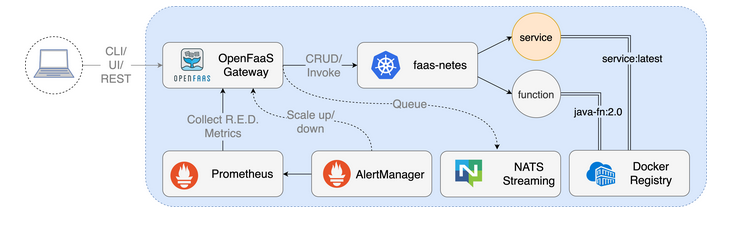
\includegraphics[width=100mm]{./thesis_images/openfaas_workflow.png}
    \label{fig:openfaas_workflow}
\end{figure}

The following are the main components on an OpenFaaS setup to give the user a
bit more intuition on how functions are scheduled, executed and scaled in the
platform. Figure \ref{fig:openfaas_workflow} goes along with the following description.

\paragraph{OpenFaaS Gateway}
\label{sec:org89b16e4}
The gateway is the entrypoint to the FaaS infrastructure. It provides an API
which opens an external route into the functions. The gateway does a lot of the
main functions in the infrastructure. The gateway is basically responsible for
collecting the metric information and scaling the functions accordingly. It has
a built in UI portal for ease of deployment and invocations of functions for the
user. When kubernetes is used as the orchestration platform, the conceptual
design of OpenFaaS can be visualized as Figure \ref{fig:openfaas_with_k8s}.

\begin{figure}[!h]
    \caption{OpenFaaS conceptual design with Kubernetes}
    \centering
    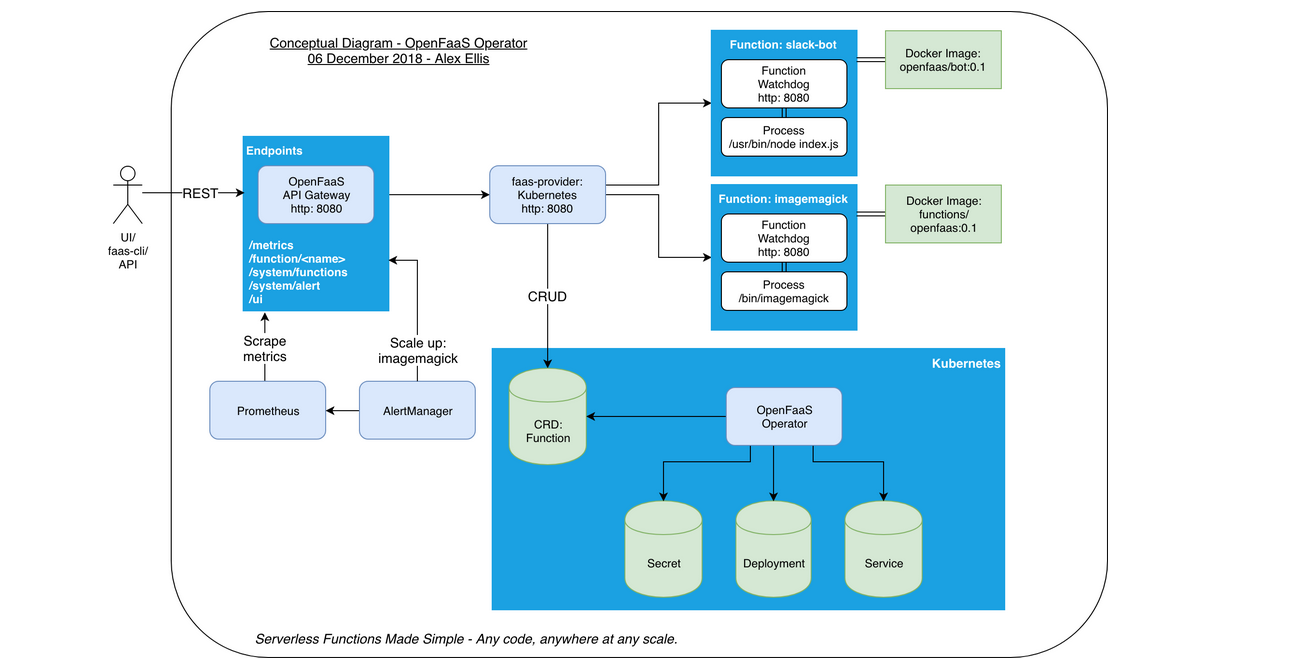
\includegraphics[width=180mm]{./thesis_images/openfaas_diag.png}
    \label{fig:openfaas_with_k8s}
\end{figure}

As can be noted in the image, Prometheus and Alertmanager are connected to the
OpenFaaS Gateway API.

\begin{itemize}
\item Prometheus is a monitoring system and time series database. Prometheus is now
the de-facto monitoring solution for Cloud Native projects. It combines a
simple interface with a powerful query language to monitor and observe
microservices and functions, which are the two primitives of any FaaS.
Prometheus basically does two functions. It gets metrics from machines in your
cluster. These machines can be actual nodes or virtual machines or containers.
One can define custom rules to check on these metrics and if any of the rules
are triggered, Prometheus will fire off alerts via AlertManager. OpenFaaS
Gateway exposes a lot of these collected metrics via Prometheus for
visualization and monitoring. We will be using these metrics for our monitoring.
\end{itemize}

\paragraph{faas-provider}
\label{sec:orgca32907}
faas-provider is a very flexible interface that provides CRUD(create, read,
update, delete) to functions and the invoke capability. The information about
the function that need to be created/updated/invoked gets fed directly from the
OpenFaaS gateway which is the endpoint to which external world communicates to.

The design of faas-provider makes OpenFaaS a unique platform. One can their own
faas-provider and hence change the backend of the OpenFaaS infrastructure very
easily. There are design guidelines available to develop your own faas-provider
backend \hyperref[ref:44]{[44}] , which basically is defining how CRUD and invoke operations
are handled by the backend. The most stable and popularly used faas-provider
that is maintained  by the community is faas-netes, which is the Kubernetes
backend for OpenFaaS.

faas-provider takes care of scheduling the functions in the right node based on
the availability and requirement. It also does the scaling up and down
of the function instances based on the information from the gateway that it
gathered via Prometheus. Figure \ref{fig:faas-provider} shows the conceptual view of just
faas-provider stripping away the rest of the complexities.

\begin{figure}[!h]
    \caption{faas-provider}
    \centering
    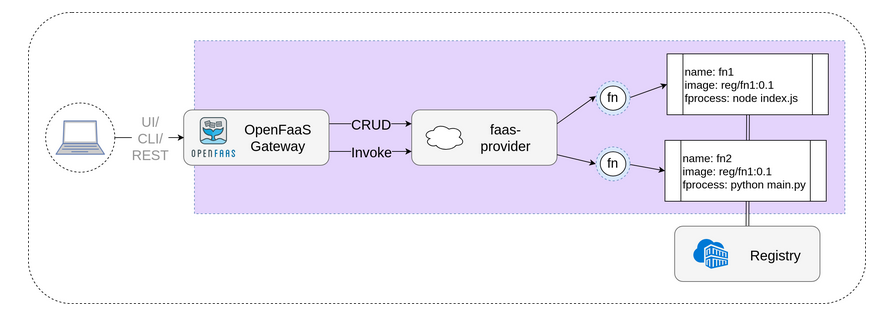
\includegraphics[width=180mm]{./thesis_images/faas-provider.png}
    \label{fig:faas-provider}
\end{figure}

\paragraph{OpenFaaS watchdog}
\label{sec:orga78a983}

The OpenFaaS watchdog \hyperref[ref:45]{[45}] is responsible for starting and monitoring functions in
OpenFaaS. Any binary can become a function through the use of watchdog.

The watchdog becomes an "init process" with an embedded HTTP server written in
Golang, it can support concurrent requests, timeouts and healthchecks. The newer
of-watchdog mentioned below is similar, but ideal for streaming use-cases or
when an expensive resource needs to be maintained between requests such as a
database connection, ML model or other data.

\paragraph{Auto-scaling}
\label{sec:org48aa853}

OpenFaaS ships with a single auto-scaling rule defined in the mounted configuration file for AlertManager. AlertManager reads usage (requests per second) metrics from Prometheus in order to know when to fire an alert to the API Gateway.

The API Gateway handles AlertManager alerts through its /system/alert route.

The auto-scaling provided by this method can be disabled by either deleting the AlertManager deployment or by scaling the deployment to zero replicas.

One can specify the minimum number of replicas and the maximum replicas to be
available. If minimum replicas is defined to be >0 then a warm copy of the
function will always be idle-ing there by avoiding the cold start issue.
Although this comes with an added cost of a docket container always up in the
memory although the resource usage during the idle time is super low. We can
also fine tune several other parameters like the factor by which the function
should be scaled up or down when there is a burst or decline of the traffic,
etc. This makes OpenFaaS extremely powerful and yet in the most simplistic way
possible.

When Kubernetes is used as the backend, instead of AlertManager the built-in
Horizontal Pod Autoscaler \hyperref[ref:46]{[46}]. This is a lot more matured as a scaler
scheduler and we will be using that for the thesis implementation.

\paragraph{NATS streaming}
\label{sec:orgf4d65aa}

A curiously lightweight application that has been adapted into OpenFaaS is NATS.
NATS provides simple and secure messaging functionality to the setup. It does
event and data streaming in the cluster. OpenFaaS uses NATS Streaming which
builds on top of the base NATS protocol to offer data streaming or a queue \hyperref[ref:47]{[47}]
. NATS streaming provides Queue worker in which the function invocation
requests can be queued up by the API Gateway, and processed in parallel when the
capacity becomes available. Asyncronous invocations can be very easily done
since it is built in without making any changes to the gateway. Each function
will have a separate endpoint that can be used to invoke it asynchronously.

NATS streaming is a Pub Sub protocol implementation like Kafka but with very
high throughput compared to the latter. Publish-subscribe  pattern  corresponds
to a mechanism where in producers publish messages that are grouped into
categories and consumers subscribe to categories which they are interested \hyperref[ref:48]{[48}]. NATS
is extremely lightweight as a
technology making it the right candidate for an elastic Serverless
infrastructure, compared to a full blown message broker
system like Kafka. Along side, considering the ephemeral nature of state in FaaS
setup, an in-memory message delivery protocol like NAT could be extremely
useful.

\paragraph{Triggers}
\label{sec:org70ee941}
OpenFaaS functions can be triggered easily by any kind of event. A small piece
of code will convert from the event-source and trigger the function using the
OpenFaaS Gateway API. Some of the most used triggers are:
\begin{itemize}
\item HTTP: One can send POST requests to the function endpoint which follows the
patter `\url{https://}<gateway URL>:<port>/function/<function name>`
\item Cron
\item NATS streaming/Async: You can execute a function or microservice
asynchronously by replacing \emph{function} with \emph{async-function} when accessing the
endpoint via the OpenFaaS gateway.
\item CLI: we can trigger user faas-cli which is a command line application to
communicate with faas gateway
\item Apache Kafka
\item AWS SQS
\item Redis
\item Minio/S3
\item RabbitMQ
\end{itemize}

\paragraph{Runtime supports and templates}
\label{sec:orgc34515f}

OpenFaaS is one of the unique engines that supports any and all programming
languages to write functions in because of its architecture. The way OpenFaaS
works, it dockerize the application by adding an of-watchdog to the application
container and deploy it to the kubernetes cluster. To make the process easier,
OpenFaaS does not expect you to write the Dockerfile. Instead, it provides
already packaged versions of language bundles called templates. The developer
can just pull the right template from the template store and just edit the
entrypoint script to add their application logic.

Like was briefly hinted earlier, OpenFaaS provides a command line tool called
faas-cli. This tool can be used to build, push and deploy the docker images from
the code. With build, it build an image into the local Docker library. With
push, it pushes that image to a remote container registry. With deploy, it
deploys your function into a cluster.

As an example, to build a simple python function, the developer will follow the
proceeding commands:

\begin{lstlisting}
faas-cli template store pull python3
faas-cli new funcname --lang python3

faas-cli build -f funcname.yml
faas-cli push funcname
faas-cli deploy -f funcname.yml
\end{lstlisting}

\subsubsection{FaaS-flow}
\label{sec:org1bf9082}
In Section 3.1, we analyzed different possible ways to do function composition.
We saw that workflow pattern is the most efficient and flexible design for a
FaaS application to composite functions. What this means is, the best way to go
about it is by keeping a Distributed Acyclic Graph in memory that is logically
sort of a flowchart defining the conditionals, branches and the loops in a
function composition.

FaaS-flow \hyperref[ref:60]{[60}] is a library written in Golang that lets the developers fiddle with
the runtime of OpenFaaS via an SDK. We will use it to orchestrate a pipeline with long running and short running
ETL jobs without having to orchestrate them manually or
maintain a separate application. Faas-flow ensures the execution order of
several functions running in parallel or dynamically and provides rich construct
to aggregate results while maintaining the intermediate data \hyperref[ref:60]{[60}].  Using
Faas-flow you can combine multiple OpenFaaS functions with little codes while
your workflow will scale up/down automatically to handle the load.

The main motivation behind the development of faas-flow is building a pipeline
that is very loosely coupled. We adapt faas-flow in this thesis considering its
extremely stateless nature. This means that the fundamental notions of FaaS
architecture is not violated here. Faas flow provides the possibility to reuse
the same function in multiple workflows which will execute in parallel agnostic
of each others execution. Along with this, in the DAG generation, faas-flow
supports multiple operations to orchestrate pipelines with conditionals,
branching, iterations, etc.

Faas flow only supports Go as a programming language for the development at the
moment which is a hard constraint. In any case this can help us build the
workflow DAGs for our proof of concept in this thesis. Now we will see some
codeblocks \hyperref[ref:60]{[60}] written using faasflow library in Go that forms certain pipeline
orchestrations.

\begin{lstlisting}
func Define(flow *faasflow.Workflow, context *faasflow.Context) (err error) \{
    flow.SyncNode()
        .Apply("func1")
        .Apply("func2")
        .Modify(func(data []byte) ([]byte, error) \{
            // do something
            return data, nil
        \})
    return nil
\}
\end{lstlisting}

The above code block defines a composition that begins by applying a function
called func1 to the start node. Then it goes ahead and apply func2. After this
we call a modify operator on the pipeline to get the data from the last pipeline
and do something with the data and return it as the end result of the whole
pipeline to the invoker. A workflow diagram of the dag can be referred from the
Figure \ref{fig:syncnode}
\begin{figure}[!h]
    \caption{Simple chaining orchestration with openfaas}
    \centering
    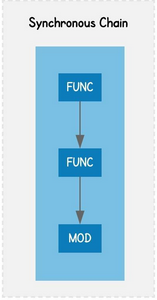
\includegraphics[width=50mm]{./thesis_images/syncnode.png}
    \label{fig:syncnode}
\end{figure}
In the above codebase though, like one could infer, the functions are in a
blocking stage. Meaning, the whole pipeline waits until each of the function
that is executing to finish before moving further down the DAG with the
execution. If there is no intermediate data to be passed along, this can
actually slow down the whole cycle. To avoid this, faas-flow supports
asynchronous chaining. The codeblock below implements an asynchronous cycle and
Figure \ref{fig:asynchrounous} represents the DAG structure of the same.

\begin{lstlisting}
func Define(flow *faasflow.Workflow, context *faasflow.Context) (err error) \{
    dag := flow.Dag()
    dag.Node("n1").Apply("func1")
    dag.Node("n2")
        .Apply("func2")
        .Modify(func(data []byte) ([]byte, error) \{
            // do something
            return data, nil
        \})
    dag.Node("n3").Apply("func4")
    dag.Edge("n1", "n2")
    dag.Edge("n2", "n3")
    return nil
\}
\end{lstlisting}


\begin{figure}[!h]
    \caption{Asynchronous function chaining}
    \centering
    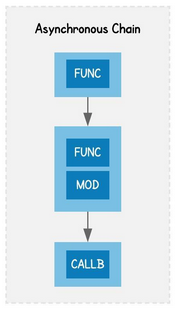
\includegraphics[width=50mm]{./thesis_images/asynchronous.png}
    \label{fig:asynchronous}
\end{figure}

Aside from these basic chaining operations, with faas-flow we can even design
orchestration that are a lot more complex like parallel branching and dynamic
branching. The following codeblock creates a parallel branching orchestration
and Figure \ref{fig:parallel} represents the DAG that is created.

\begin{figure}[!h]
    \caption{Parallel execution function chaining}
    \centering
    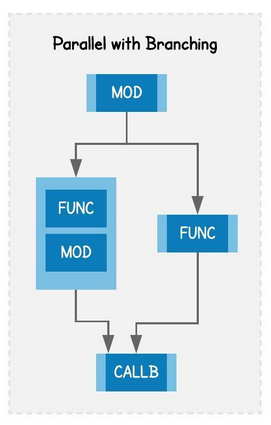
\includegraphics[width=50mm]{./thesis_images/parallel.png}
    \label{fig:parallel}
\end{figure}
\begin{lstlisting}
func Define(flow *faasflow.Workflow, context *faasflow.Context) (err error) \{
    dag := flow.Dag()
    dag.Node("n1").Modify(func(data []byte) ([]byte, error) \{
        // do something
        return data, nil
    \})
    dag.Node("n2").Apply("func1")
    dag.Node("n3").Apply("func2").Modify(func(data []byte) ([]byte, error) \{
        // do something
        return data, nil
    \})
    dag.Node("n4", faasflow.Aggregator(func(data map[string][]byte) ([]byte, error) \{
        // aggregate branch result data["n2"] and data["n3"]
        return []byte(""), nil
    \}))

    dag.Edge("n1", "n2")
    dag.Edge("n1", "n3")
    dag.Edge("n2", "n4")
    dag.Edge("n3", "n4")
    return nil
\}
\end{lstlisting}

Faas flow does not use a complete workflow based approach for the orchestration.
Instead it mixes it with an event based workflow. Meaning that, internally
faasflow keeps a DAG, but the completion of each node in the DAG is broadcasted
with the help of an event queue. faas-flow uses NAT streaming \hyperref[ref:47]{[47}] as the event
bus. Node execution in Faas-flow starts by a completion event of one or more
previous nodes. A completion event denotes that all the previous dependent nodes
have completed. The event carries the execution state and identifies the next
node to execute. With events Faas-flow asynchronously carry-on execution of
nodes by iterating itself over and over till all nodes are executed. Figure
\ref{fig:nat} logically represents how function orchestration happen via event
propagation.

\begin{figure}[!h]
    \caption{Event based workflows}
    \centering
    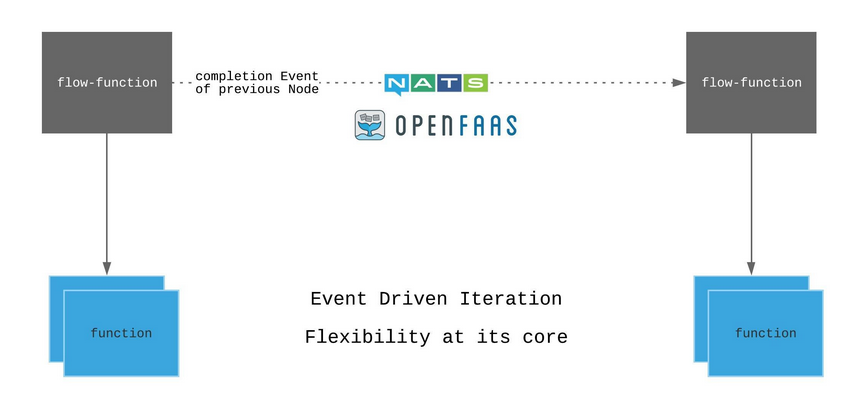
\includegraphics[width=130mm]{./thesis_images/nat.png}
    \label{fig:nat}
\end{figure}

The most notable thing about faasflow is its flexibility and extensibility as a
tool. We can extend faas flow to add different kind of storage infrastructures
to the workflow. Faas flow basically has two kind of data. First is the state of
the DAG that is being processed by faas flow and then is the intermediate data
that need to be transferred between two functions. The former is called the state
store and the latter is called the data store.  We can write our own libraries
to define our own data store and state store logic and how we want to deal with
data in the pipeline. Figure \ref{fig:statestore} and Figure \ref{fig:datastore}
represents the logical workflow when we add external storage suits.

\begin{figure}[!h]
    \caption{State store logical view}
    \centering
    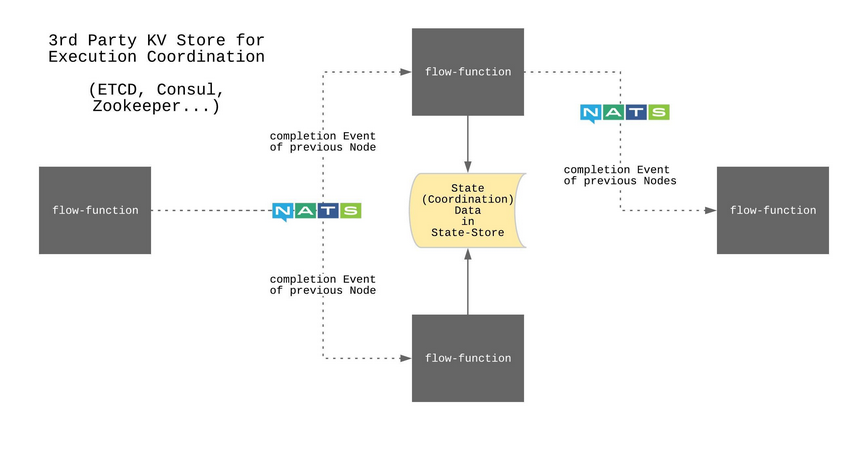
\includegraphics[width=100mm]{./thesis_images/statestore.png}
    \label{fig:statestore}
\end{figure}

\begin{figure}[!h]
    \caption{Data Store logical view}
    \centering
    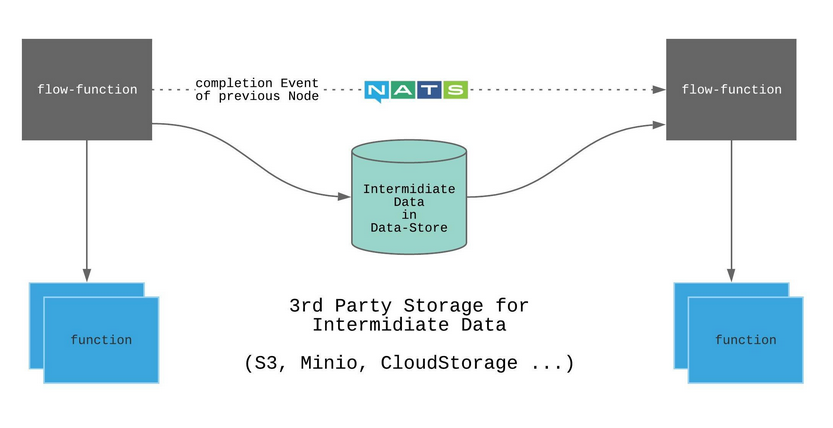
\includegraphics[width=100mm]{./thesis_images/datastore.png}
    \label{fig:datastore}
\end{figure}

Another important thing about faas flow is that faas flow at the end of the
works as yet another function in the FaaS infrastructure letting it leverage the
autoscaling policies of the system than handling it itself. There rich features
make us adapt faas-flow as the choice of orchestration engine for our proof of concept.

\subsubsection{Prometheus}
\label{sec:orgf510957}
In the previous section, we discussed briefly about the time-series monitoring
approach adapted by Google. Prometheus is an Open Source monitoring and alerting
toolkit that works exactly the way Google Borgman works. The working of
Prometheus is rather curious. We can statically configure Prometheus to detect
certain metric sources. For example, the CPU usage of the nodes in the
Kuberenetes cluster. Prometheus pulls these metric as a time-series over HTTP.
Prometheus need not be setup in the same cluster as the applications. Prometheus
does not even expect to be run as a distributed system. At this stage, Prometheus
parses the data and keep a a multi-dimensional data model with time series data
identified by metric name and key/value pairs. There are streams of timestamped
values belonging to the same metric and the same set of labeled dimensions \hyperref[ref:49]{[49}]
. Prometheus also comes with a query language called PromQL that can
query over streaming, multi-dimensional time series data.

Prometheus is a tool that is written in Go programming language. The main
component of Prometheus is a server that scrapes the time series data.
Prometheus packs several client libraries that need to be used in application
code if data has to be pushed to Prometheus. For ephemeral jobs that are
shortlived, as is the case with most FaaS functions, Prometheus provides a push
gateway. The Prometheus Pushgateway exists to allow ephemeral and batch jobs to expose
their metrics to Prometheus. Since these kinds of jobs may not exist long enough
to be scraped, they can instead push their metrics to a Pushgateway. The
Pushgateway then exposes these metrics to Prometheus \hyperref[ref:50]{[50}]. There are
several other exporters for various services. Along with various other support
tools, Prometheus also has an inbuilt alert manager to handle alerts. Figure \ref{fig:prometheus}
shows the overall system architecture of Prometheus.

\begin{figure}[!h]
    \caption{Prometheus Architecture}
    \centering
    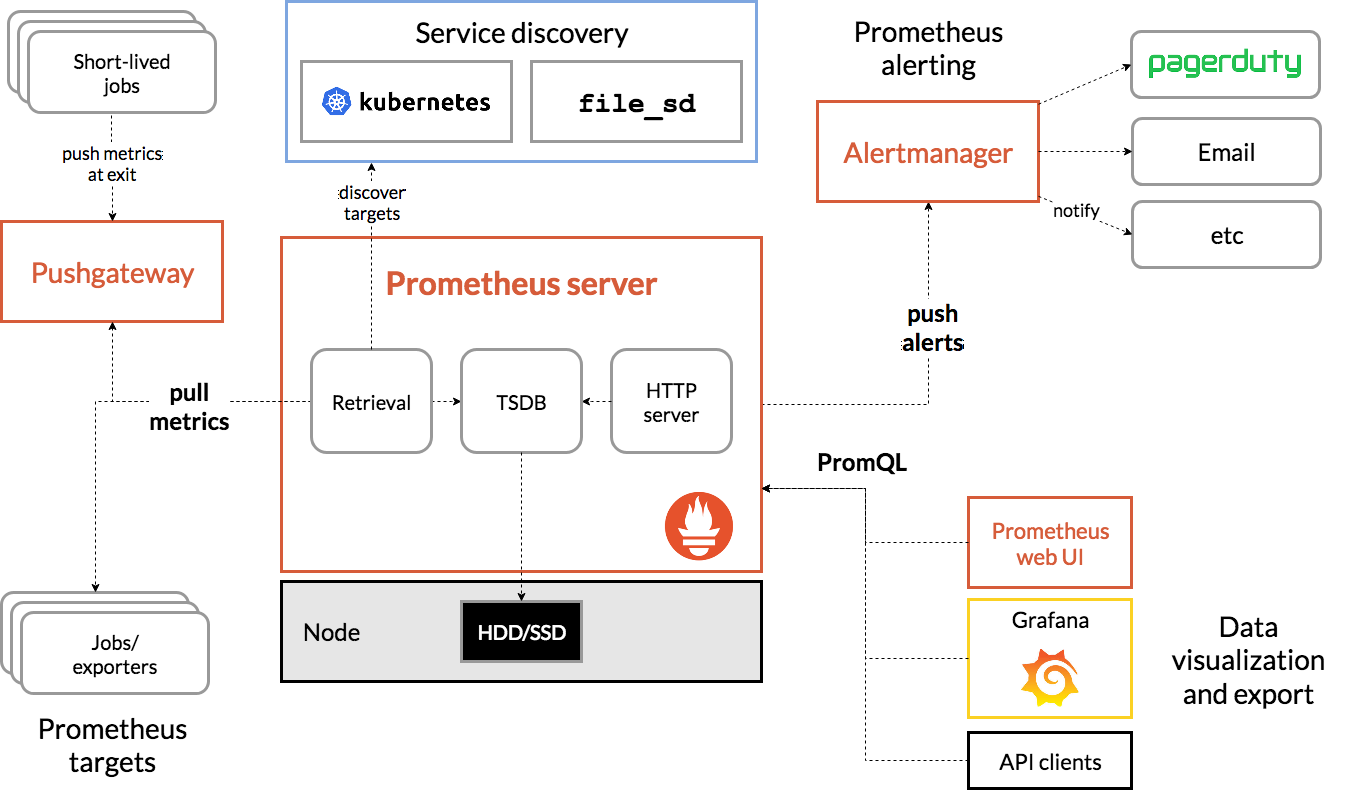
\includegraphics[width=130mm]{./thesis_images/prometheus.png}
    \label{fig:prometheus}
\end{figure}

There are numerous tools that can be used to connect to Prometheus like Grafana
that lets us visualize the data with more meaning in a dashboard. Prometheus can
be used with any kind of numeric data. May it be machine-centric monitoring or
monitoring of highly dynamic service-oriented architectures. We can track the
usage of the system resources via Prometheus in a very fine grained manner.
Memory, CPU, and execution time of the application, all can be accounted for as
a function of time. The person maintaining our system can do fine grained
billing using these usage metric.

OpenFaaS Gateway component exposes several metrics to help you monitor the
health and behavior of the functions. We will leveraging that to have clean
usage tracking for our system. For example, to get the total number of
successful function invocations from the gateway, we can run the PromQL query
\emph{sum( gateway\textsubscript{function}\textsubscript{invocation}\textsubscript{total} \{  code=$\backslash$"200$\backslash$"\}}



\subsubsection{Jaeger}
\label{sec:org3ceefc6}
We discussed how OpenTracing API helps identify the bottlenecks and allows easy
debugging in a distributed setup. One of the most popular implementations of
OpenTracing API is Jaegar \hyperref[ref:51]{[51}]. Jaeger identifies that the difficulty in
dealing with debugging in microservices or FaaS setups are an order of magnitude
away from simple monoliths. The majority of operational problems happen in such platforms
either as an issue of networking or that of observability.

We already mentioned Spans and Traces as a part of OpenTracking API in the
previous section. One think special about Jaeger is that, it handle trace as a
directed acyclic graph of spans. This basically visualizes the data/execution
path through the system.

\begin{figure}[!h]
    \caption{Jaeger Architecture}
    \centering
    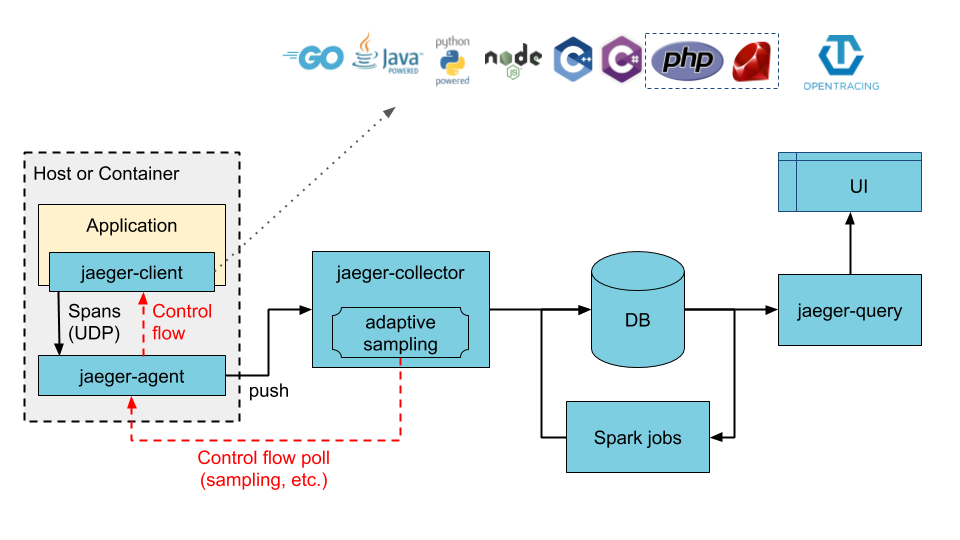
\includegraphics[width=130mm]{./thesis_images/jaeger.png}
    \label{fig:jaeger}
\end{figure}

Figure \ref{fig:jaeger} shows the architecture of Jaeger. Jaegar has code facing client libraries
that are compliant with OpenTracing API. It can be integrated very easily with
any tool that is integrated with OpenTracing. This includes frameworks like
Flask, gRPC, and many more. Basically an instrumented service creates spans when
receiving new requests and attaches context information (trace id, span id, and
baggage) to outgoing requests \hyperref[ref:52]{[52}]. Sampled spans are propagated out of
the process asynchronously to Jaeger Agents. This process has very little
overhead. The Jaeger agent is a network daemon that listens for spans sent over
UDP, which it batches and sends to the collector. It is designed to be deployed
to all hosts as an infrastructure component. Collective receive these traces and
process it to validate, index, transform and store them. Like Prometheus, Jaeger
also supports a Query language via a Query component and visualizes the output
in a UI. Figure \ref{fig:jaeger_traces} shows what the UI looks like for a web app on an HTTP request to
the endpoint.
\begin{figure}[!h]
    \caption{Jaeger UI}
    \centering
    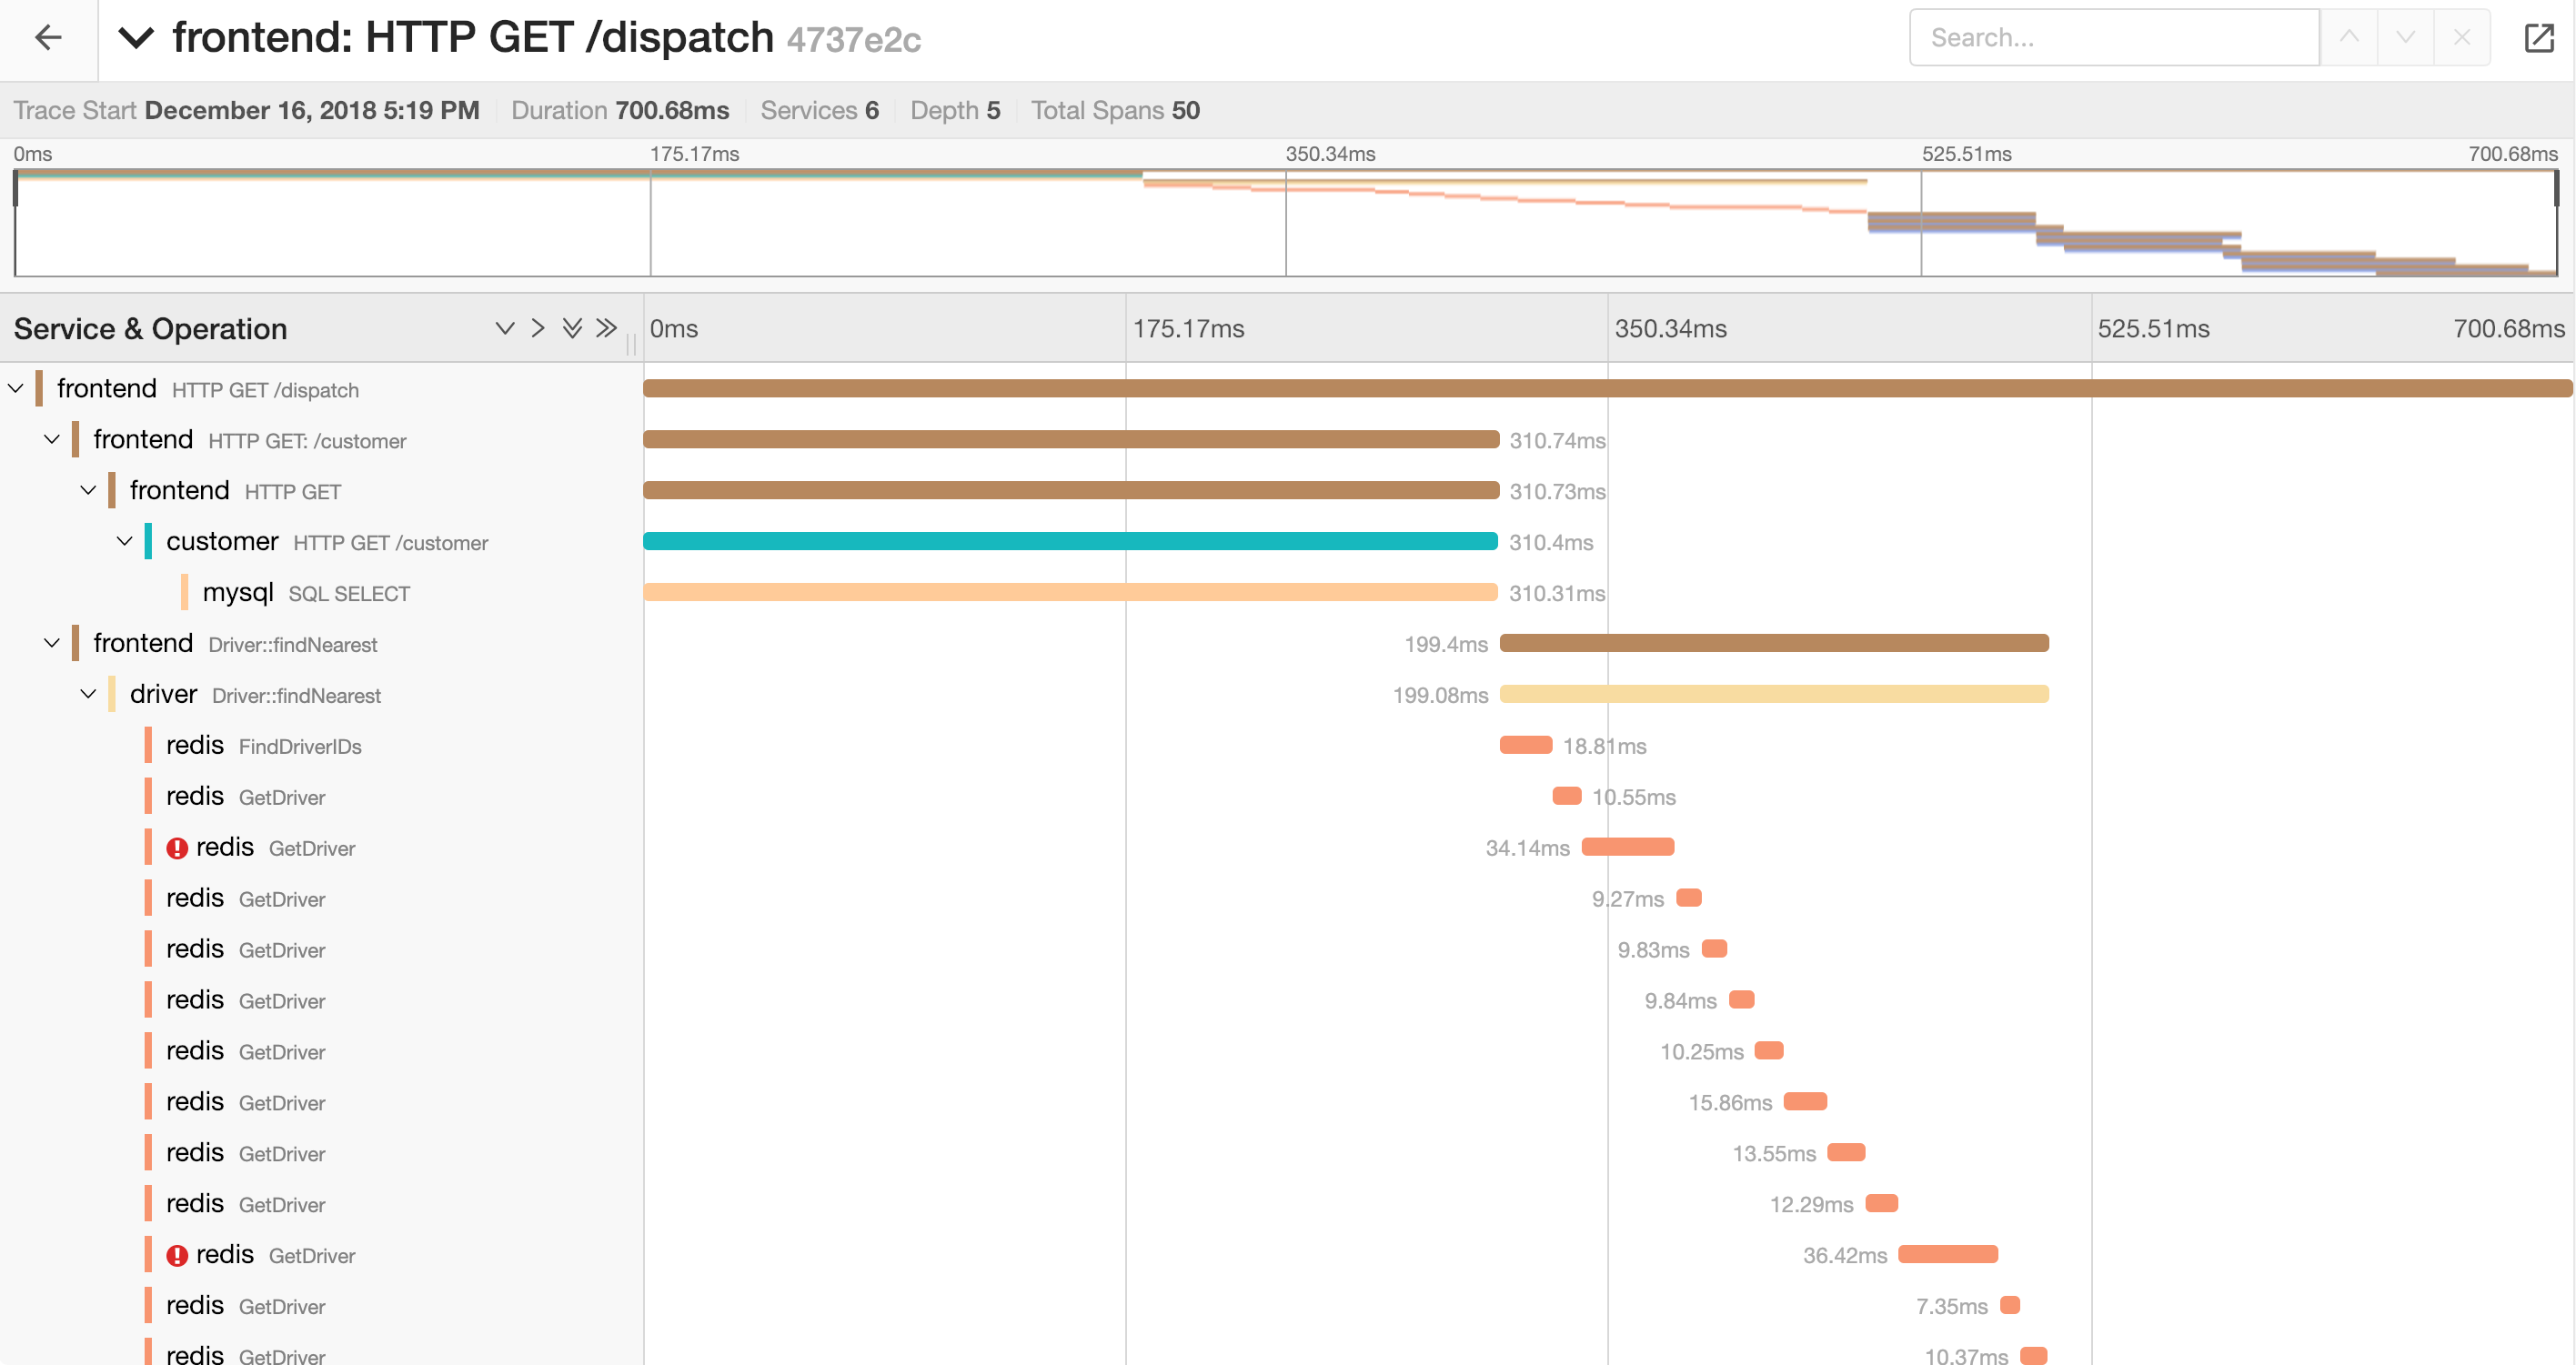
\includegraphics[width=130mm]{./thesis_images/jaeger_traces.png}
    \label{fig:jaeger_traces}
\end{figure}

\subsection{Architecture Overview}
\label{sec:org6872281}
In this section, we will see how the tools mentioned above were efficiently used
to build an orchestration system for pipelined FaaS workloads that work much better than
the out of the box solutions. Great care was given into building a system that
is very easy to deploy and maintain for the infrastructure providers. We believe
that the practicality, adaptability and the accordance with the core
philosophies of serverless architecture make our system unique.

We can separate our system logically into 3 parts. The FaaS runtime, the
workflow framework and the workflow defining client API. The functions that are
(written in any language of preference) that does the computations exist outside the
logic.

Figure \ref{fig:arch} depicts the overall architecture of the setup. To begin
with, we have the OpenFaaS runtime which takes care of the execution of the
function instances upon triggers using Kubernetes and packaging the functions as
Docker containers. We configure the setup to not scale down to zero to avoid the
cold start time during the initial start. We might still incur a bit of cold start
when the number of instances is scaling up upon heavy load.

By default in OpenFaaS, functions are coupled with a tiny Go based server and a
function watchdog \hyperref[ref:45]{[45}]. The watchdog takes care of parsing the incoming requests
and forwards it to the function via standard IO. There is no latency between
this call transfer since it happens internally and the watchdog process is
co-located with the function instance. In our implementation though we remove
the watchdog component from the function runtime since our added framework for
the workflows take care of handling the requests and passing it between the
functions. We try to avoid the added latency by the watchdog process since we
already serializes and de-serializes the data as a part of data store library.
This also means that we can test the efficiency of the orchestration setup
without the added latency by the platform. OpenFaaS’ runtime driver for
Kubernetes is faas-netes, which deploys functions as Kubernetes pods, and then
delegates scheduling decisions to the Kubernetes scheduler.

We keep the NATS streaming message queue that is used by faas-netes for queuing
of requests. The interesting thing about the NATS streaming here is that, the
storage is in-memory only of the queued requests. This is rather interesting
because it means that the message queue is completely autoscalable as well since
we have the RAM pool controlled by the Kubernetes autoscaling logic. This helps
in keeping our platform completely elastic.

The requests received by the gateway are queued in the NATS streaming. The
workflow function orchestrated using faas-flow will receive these messages from
the queue. The workflow framework takes care of handling the request arriving,
formatting it in the way needed. Then the DAG is processed with the input data
by the framework. The DAG or the workflow is a part of the state that the
OpenFaaS runtime need to process. The whole workflow is basically stored in the
state store along with the current state of the workflow which can be retrieved
by the workflow framework from time to time to trigger the next function that
needs to be executed. Whenever a function finishes its execution a FINISH event
is sent to the message queue which is the NATS streaming, which triggers the
workflow framework to fetch the next node to be executed from the state store
and trigger it over HTTP via the OpenFaaS gateway. At the end of each function,
a call is made to the OpenTracing setup to register the span of each function
invocation which can be used for evaluation and optimizations. Once the
execution of a particular node is over, the information about that node in the
flow is removed from the state store and there by automatically freeing up memory.

\begin{figure}[!h]
    \caption{Architecture}
    \centering
    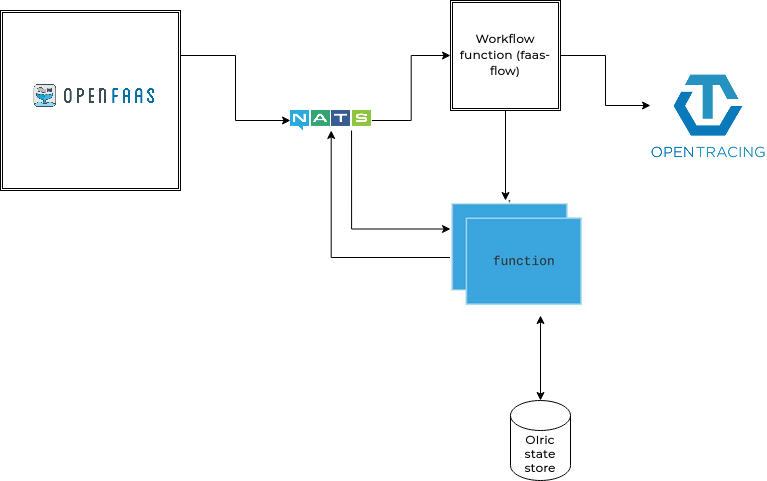
\includegraphics[width=130mm]{./thesis_images/architecture.png}
    \label{fig:arch}
\end{figure}

The data returned from any of the function invocations are stored in an
intermediate data store provided by us. This data is ephemeral in nature and
exists in memory only until the workflow has successfully finished execution.
There is a request id parameter associated with the particular invocation of a
node or instance. The data stored will use this request ID to identify it
uniquely and is fetched by the following function accordingly.

\subsubsection{Workflow framework}
\label{sec:orga986456}
The workflow framework is the most important part of our orchestration platform.
We discussed in section 3.1 different theoretical solutions for composing
functions. From the analysis it was quite clear that the workflow based
orchestration provides the most amount of flexibility and scalability to the
system. The problem of introducing something like that directly to Serverless
platform is the complication in maintaining the state. Since we have multiple
functions getting triggered(asynchronously at times), it gets really hard to
realize if a function has terminated and might even lead us to a polling sort of
methodology which is kind of inefficient. Instead we choose to mix event based
orchestration to workflow orchestrations.

The user communicates with the system via the client library. This is a form of
domain specific format to specify the structure of the Directed Acyclic Graph.
We use the faas-flow interface language to provide the client library. This was
explained in detail in section 4.1.3. By default, OpenFaas runtime takes caring handling events from function like
function termination, function error, etc. We cannot use this inherent ability
since we want our workflow to proceed differently that the conventional way.
Hence we tweak the function runtime to override the default event handler and
the function executor in the OpenFaas platform. We make each functions sent out
events to the event queue after the execution completion, on errors, etc. Upon
receiving these events, our workflow runtime will look inside the state store
for the next node/function to be executed according to the DAG specified via the
client library and the respective function is triggered. The workflow library
globally keeps a context map for each invocation. The context map contains the
current node which is the current node/function of execution, state which
represents the orchestration structure and the requestID which is a unique
identification for the current request invocation. Like was mentioned earlier,
this is used while storing the function intermediate data of each invocation.

Along with the orchestration, workflow framework takes care of the trace
handling. Each function can take three states during their lifetime - Running,
Paused, Stopped. On each of this state update via the events, the framework
sends logs a corresponding entry on the OpenTracing platform. This is how the
spans and traces are logged in the system.

Using the standard visual interface of OpenTracing, we can visualize these
tracing information which would look similar to Figure \ref{fig:tracing}. Like is
visible, there is a request ID representing the trace of the entire
orchestration. Then you can see the spans of each node in the graph(function in
composition). It is easy to measure the latency of each step via this interface.

\begin{figure}[!h]
    \caption{Trace of a sample workload}
    \centering
    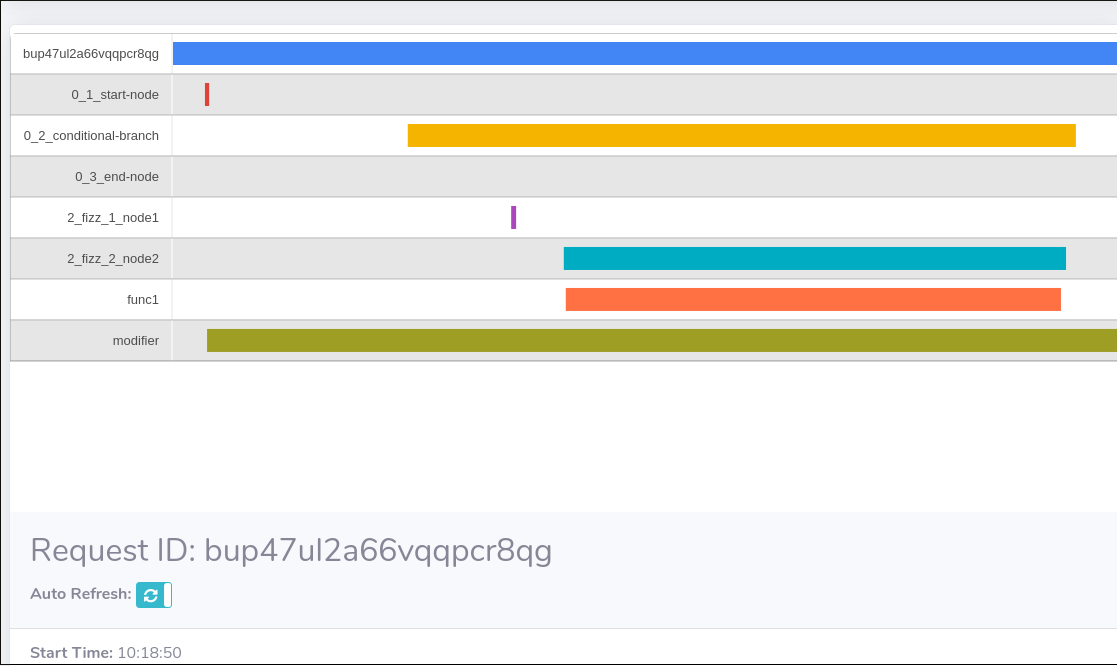
\includegraphics[width=100mm]{./thesis_images/tracing.png}
    \label{fig:tracing}
\end{figure}

Along with this interface, we use a D3 based library setup to visualize the DAG
structure that represents our function orchestration. Figure \ref{fig:dag} shows
how the DAG looks like in our setup for a sample code that modify data based on
a conditional "odd or even". The blocks composing the modify nodes are the ones
that change the data or have side effects if we talk in a functional language paradigm.

\begin{figure}[!h]
    \caption{DAG of a sample workload}
    \centering
    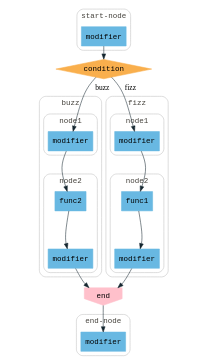
\includegraphics[width=50mm]{./thesis_images/dag.png}
    \label{fig:dag}
\end{figure}

There are certain configurable parameters in the system. We can enable or
disable the tracing, we can set the whole system to scale from 0 than from 1, we
can set an upper limit to the amount of memory and CPU used by the system, etc.
The standard OpenFaaS config \hyperref[ref:63]{[63}] support is used for this but we found it quite
flexible and easy to use.

\subsubsection{Data store library}
\label{sec:org46f384f}
To store the ephemeral data between the functions like was mentioned earlier we
propose the usage of distributed in-memory cache which can be easily scaled up
and down. Our consideration was both Pocket and Olric. For the implementation
though, due to technical difficulties we opted the usage of Olric.

Olric was deployed as Kubernetes pods one per each node in the cluster to ensure
that the data transfer time among the storage and the functions are minimum. To
communicate to this library, we added a data store management library for Orlic
extending the faas-flow library \hyperref[ref:64]{[64}].

The library integrates effortlessly with the DataStore object of faas-flow
library. The DataStore interface of faas-flow first looks for a Init endpoints
that initializes the connection with the deployed Olric setup, configures the
timeouts and maximum number of connections. The Olric Go library is used to
build the interface. During this initialization step we also specify the
serialization library that needs to be used. We use Go's NewMsgPack as the
serialization library. MessagePack \hyperref[ref:65]{[65}] is a binary serialization format that
functions a bit like JSON. Small integers are encoded into a single byte, and
typical short strings require only one extra byte in addition to the strings
themselves. This makes it a bit better than JSON in the performance.

For each new request that is created on the faas-flow pipeline, our library
creates a new distributed map to store the key value pairs. On the termination
of the request, this distributed map is deleted. Alongside we take of the logic
to set and get values to and from the distributed map during the FINISH and
RUNNING event changes on the workflow framework. The handling of the events are
done inherently by faas-flow as was explained earlier.

\subsubsection{Monitoring \& usage tracking}
\label{sec:org1072a69}
We looked in detail at Prometheus as a monitoring tool in the previous section.
As a part of the thesis implementation, we deployed Prometheus and Grafana to
monitor the usage of the resources and scaling of the platform. The data needs
to be appropriately exposed and formatted so that Prometheus can collect it.
Prometheus can access data directly from the app’s client libraries or by using
exporters. An exporter is a piece of software sitting next to the application
that sends data to prometheus to scrape. Exporter basically accepts HTTP request
from Prometheus and provide the data to Prometheus. For Prometheus to know what
data to pull, it uses a Service Discovery. For example, In the case of
Kubernetes cluster, this Service Discovery is done via Kubernetes API since it
already has labels, names, etc. for all the applications in it. Figure
\ref{fig:service_disc} shows the way Prometheus connects with applications and
process the data.

\begin{figure}[!h]
    \caption{Prometheus workflow}
    \centering
    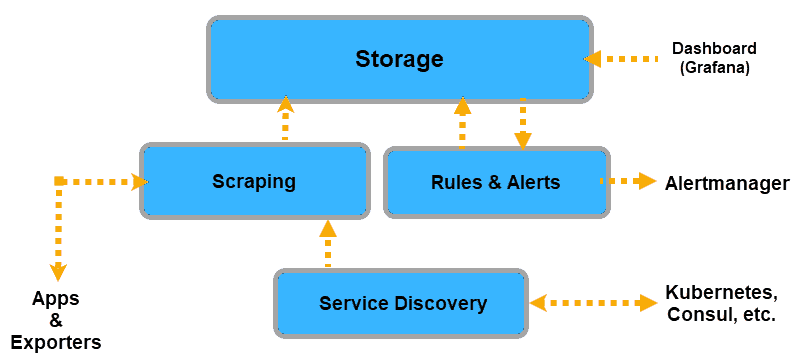
\includegraphics[width=80mm]{./thesis_images/service_disc.png}
    \label{fig:service_disc}
\end{figure}

Along with the application information, we should get information about the
nodes such as disk usage, CPU usage, etc. We use node exporter \hyperref[ref:66]{[66}] for this. Along
with this, we also have to export the information about the cgroups that make up
Docker containers. For this we use Google's cadvisor project \hyperref[ref:67]{[67}]. Once this
connection is made, we can use the PromQL language to query from the scraped
time series data.

Prometheus can be easily installed on Kubernetes with the help of YAML
configurations. Then in the configuration to specify the scraper called
scape\textsubscript{config}, provide the Kubernetes API, kubectl. The output of the PromQL
queries can be used to track the usage by the applications in the infrastructure
along with the responsiveness of the system with respect to the scaling, etc.
Figure \ref{fig:monitoring} represents a monitoring visualization setup for a
serverless infrastructure.

\begin{figure}[!h]
    \caption{Grafana Visualization of Prometheus data}
    \centering
    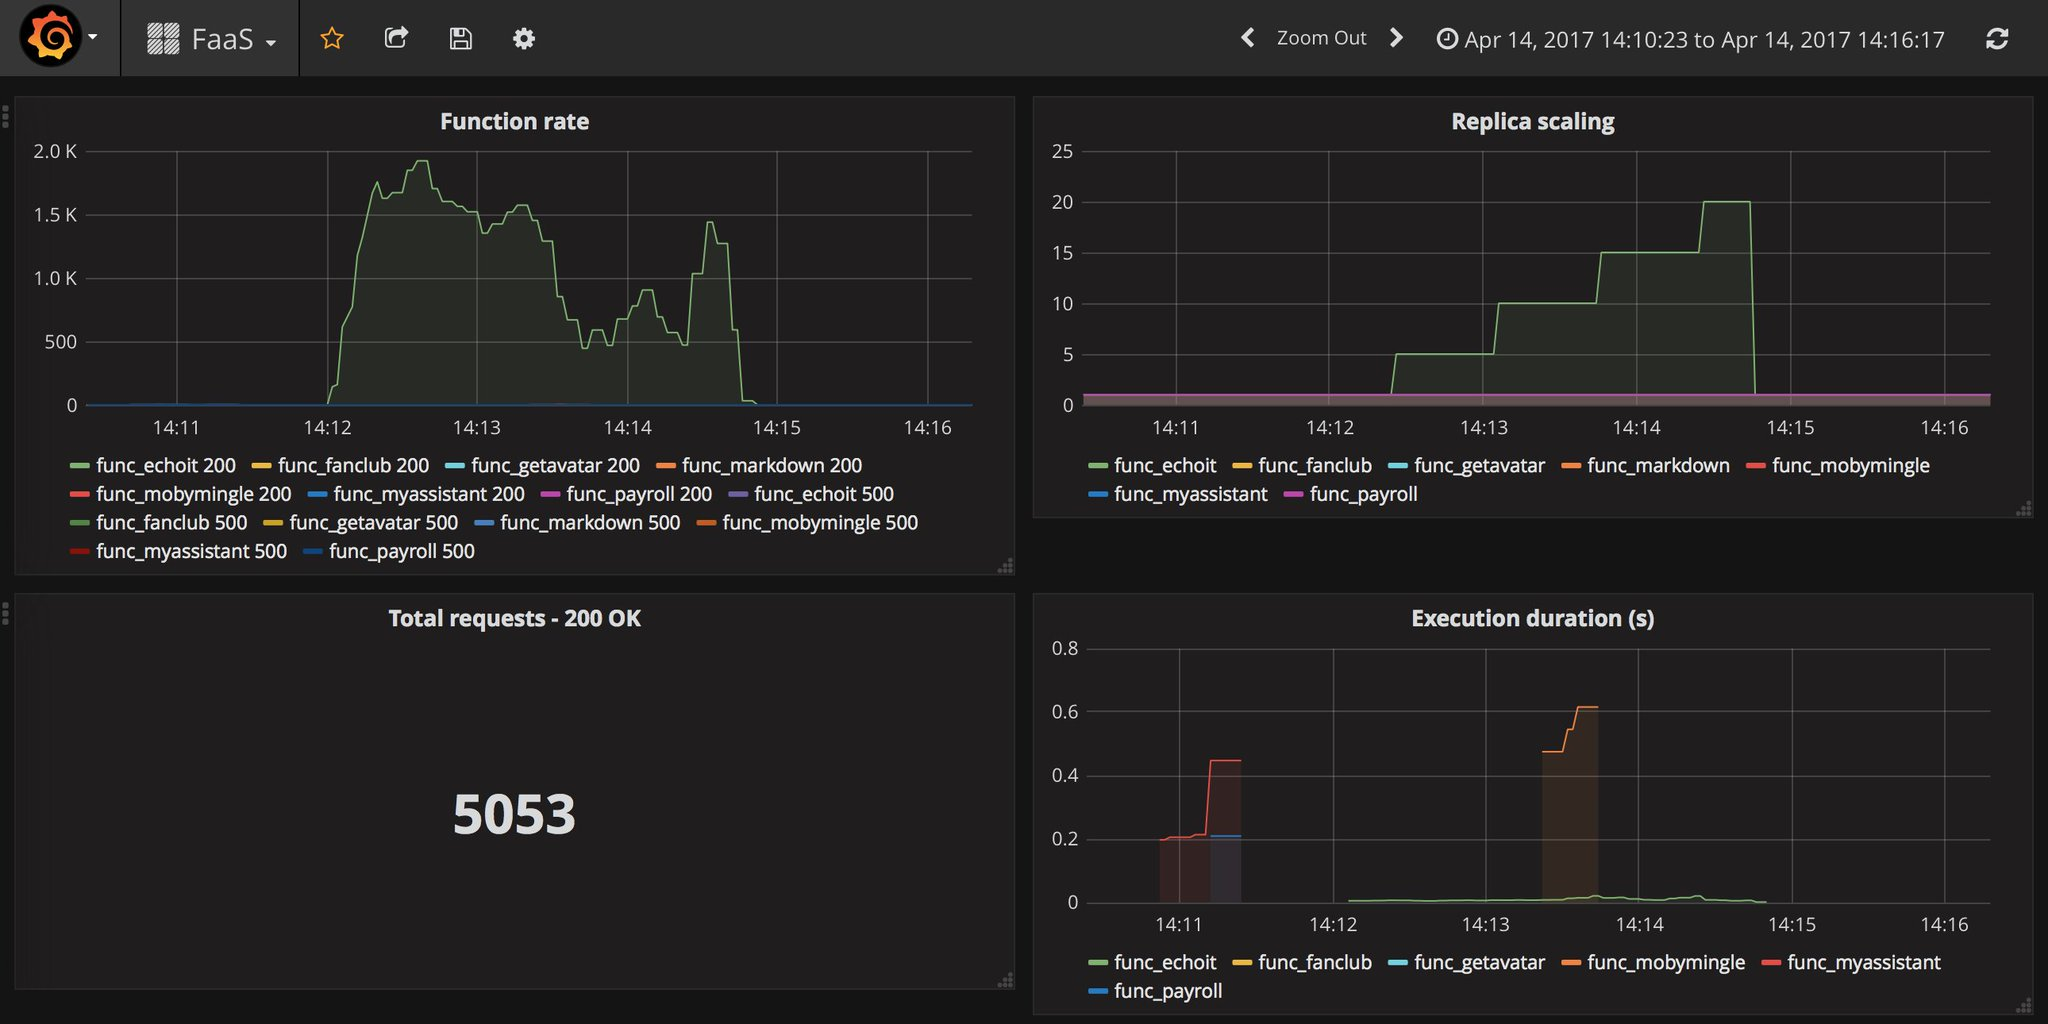
\includegraphics[width=150mm]{./thesis_images/monitoring.jpeg}
    \label{fig:monitoring}
\end{figure}

\section{Evaluation}
\label{sec:org75a97b7}
To analyze the efficiency of our system, we thought of the right kind of metrics
that would quantitatively measure the improvement in the issues we were trying
to resolve. We wanted to understand how the composition technique and the
ephemeral storage affects the following aspects of the system:
\begin{itemize}
\item Overall pipeline execution
\item Individual function execution
\item Scaling of individual functions
\item Resource usage
\end{itemize}

We are not measuring the cold start latencies of the system since the mechanism
we proposed would not alter anything in this scenario. Also our system 
maintain a warm pool of instances to avoid the initial cold start latency.  

To empirically evaluate the above mentioned aspects, we track several metrics
via the monitoring and tracing systems we have setup for the infrastructure. For
each workload we test, we record the following details:
\begin{itemize}
\item \textbf{Trace of the whole function orchestra (Overall execution time):}
Overall execution of a function orchestra comprises usually comprises the cold start
time, the time to store and retrieve intermediate data and the function
execution of the whole pipeline. We are hoping to find a reduction in the
execution time on our proposed solution.
\item \textbf{Span of individual function (Single function execution time):}
Our tracing platform effectively records the span of each function. We expect
a reduction here as well.
\item \textbf{The percentage of requests that were handled by the system:}
We measure the number of requests that hit the OpenFaaS gateway the number of
successful requests. This measures if our system ever drops a request during
heavy load situation. A successful execution is considered as the ones that
return 200 status code. We can measure this value for each second and
calculate the throughput of the system. We will set a 30s timeout on open requests which will
be marked as failed.
\item \textbf{Memory and CPU usage:}
We measure the Memory and CPU usage by each pipeline. This is to learn if our
method produced any unexpected spikes in CPU usage and memory and also to test
our theory on having a easily billable infrastructure.
\item \textbf{Scaled parameter:}
We define a scaling logic for our setup. We will measure the responsiveness of
the platform to heavy load, how easily it scales up and down.
\end{itemize}

For measuring the improvement our thesis has made to the platform, we compare the platform with the standard practices used for function
orchestrations using OpenFaaS. We choose to stick to testing workload on the
same platform since certain latencies are very much platform dependent. It
would not be very enlightening if we compare a setup of our thesis on OpenFaaS to
a commercial setup like AWS Lambda. We design our workloads on OpenFaaS in three different ways:
\begin{itemize}
\item \textbf{Manual orchestration:}
We compose the functions by issuing an HTTP request from each other which is
the suggested way of doing it by AWS in the absence of step functions \hyperref[ref:21]{[21}].
\item \textbf{Orchestration with faas-flow and object store:}
We compose the functions using faas-flow but use an object store for storing
the intermediate data that needs to transferred between the functions
\item \textbf{Orchestration with faas-flow and state store:}
Here we compose the functions with faas-flow but use the in-memory data store
for the intermediate storage
\end{itemize}

\subsection{Setup and tools}
\label{sec:org7f4fd0b}
For the proof of concept, We setup OpenFaaS on single node Kubernetes cluster
setup on AWS. 
Each machine has 2 vCPUs and 8GB of dedicated memory. We used the
helm charts \hyperref[ref:68]{[68}] of OpenFaaS to setup the FaaS platform. We extended or
removed memory limits / quotas for each service and function.
For the test setup we turn off the debug flag so that the logs for the function
are kept sparse. Like was mentioned in the Implementation section, we connect
Prometheus, Grafana and Jaeger tracing with the setup to get fine grained usage
and runtime data from the environment. It is worth noting that we use minikube \hyperref[ref:71]{[72}]
to setup the cluster which technically runs over KVM hypervisor. This introduces
some latency to the setup.

In the same cluster we setup Olric, the in-memory distributed cache of our
choice, with one pod in each of the nod in the cluster. We connect Olric to
Prometheus to get the usage of the memory by the state store. To test our second
type of orchestration, the one with the object store, we chose an Open Source
object store called Minio \hyperref[ref:69]{[69}]. Minio has the functionalities very similar to
AWS s3 with an almost similar CLI library. We use the pre-built helm charts of
Minio as well for the setup.

One we had the whole setup ready, we configured the platform to have no limits
over scaling factor of the function. Along with this we define the rule for
scaling the function instances. We make this a function of the number of
invocations to have a load based scaling strategy. Like was discussed during the
description of OpenFaaS, AlertManager is responsible for firing requests for
scaling up and down to the OpenFaaS gateway as per the metrics tracked by
Prometheus. So we write the custom AlertManager rule on Prometheus with PromQL.
The logic we specify is as follows:
\begin{lstlisting}
alert: APIHighInvocationRate
expr: sum(rate(gateway-function-invocation-total\{code= "200"\}[10s])) BY (functionName) > 5
for: 5s
\end{lstlisting}
The above query groups the invocation by the function name. If the sum of
successful invocations is above 5 within 5 seconds, the gateway scales up the
function instances running by a certain factor. We define this factor to be 20\%
in the OpenFaaS configuration file for our functions later.

For load testing we use the HTTP load mocking library called hey \hyperref[ref:71]{[71}]. hey is a
lightweight replacement for ApacheBench. hey runs provided number of requests in
the provided concurrency level and prints stats. It can be used as a command as
follows:
\begin{lstlisting}
hey -q 1 -c 1 -z 15m 'http://<server-ip>/function/nodeinfo'
\end{lstlisting}
The above command sends 1 request per second for a total of 15 minutes to the
function called nodeinfo in the local OpenFaaS setup.

\subsection{Workload}
\label{sec:orgd5fdc8a}
We use a very simple workload to do the function composition with. We implement
the famous Fizz buzz children's puzzle \hyperref[ref:70]{[70}]. It is a simple function that checks
if a number is divisible by 5, in which case it replaces the number with buzz
and if it is divisible by 3, the number is replaces by fizz. We split this into
multiple functions. The first function checks if the number is divisible by 3 or
by 5 and conditionally it chooses the next function which either is: the
function that return fizz, the function that returns buzz, or the function that
returns the same number. This function is great because we can test the
conditional branching in the composition. It is not particularly CPU intensive
or memory intensive. We do not want such workloads since our scaling heuristics
depend on the number of requests.

Figure \ref{fig:fizz_buzz} shows the DAG generated from the composition. Like
one can notice, based on the conditional(divide by3, divide by 5, or neither)
the flow can take one of three branches. At the end, the end node returns the
value in a unified format.

\begin{figure}[!h]
    \caption{Fizz buzz workload}
    \centering
    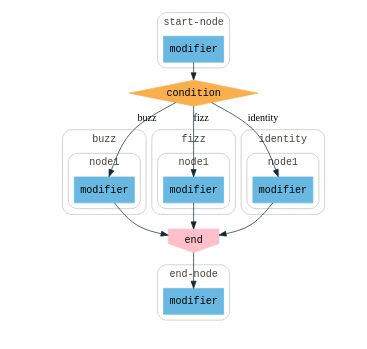
\includegraphics[width=80mm]{./thesis_images/fizz_buzz.png}
    \label{fig:fizz_buzz}
\end{figure}

\subsection{Results and Analysis}
\label{sec:orgdd708c0}

To begin the experiment with we used hey command line tool to produce three
different kind of load for the above three different workloads. We tried a load
of 1 request every 1 second for 1 minute, a load of 50 requests concurrently for 40 seconds.
We noted the metrics on hey, average spans on the tracing framework, scaling
frequency and the CPU and memory usage for all the mentioned workloads as
follows:

\subsubsection{faas-flow with ephemeral storage}
\label{sec:org8052481}

In the first setup we try emulate an HTTP load of one request per second for a
whole minute using the testing tool hey like mentioned earlier. The command
would be as follows:
\begin{lstlisting}
hey -q 1 -c 1 -z 1m 'http://<server-ip>/function/fizz-buzz-olric'
\end{lstlisting}
We notice that all 60 requests that were sent were successfully handled by the
platform. We get the benchmark information from hey like is shown in Figure \ref{fig:fizz-buzz-olric}.
\begin{center}
   \begin{minipage}{\linewidth}
     \centering
    \captionof{figure}{Benchmark summary from hey for composition with ephemeral storage}
    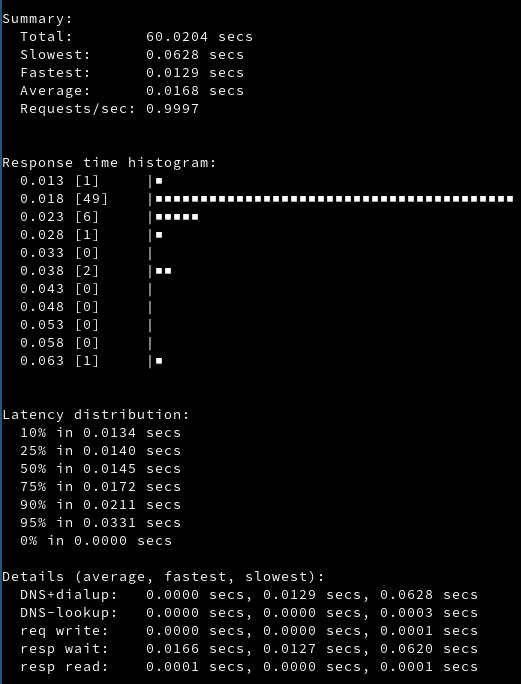
\includegraphics[width=100mm]{./thesis_images/real-fizz-1.png}
    \label{fig:fizz-buzz-olric}
\end{minipage}
\end{center}

It is seen that on average the pipeline took 0.0168 seconds.

Further looking at the function span, it can be seen that the starting node in the
composition is the one that takes up the most time in the execution. On average
this is seen as 0.013s.

We try increasing the load on the function so we can see how well it scales. We
invoke an HTTP mock load of around 200 requests per second for a period of 1 minute. 
All of the requests were handled by the platform. The hey benchmarking details
are as in Figure \ref{fig:real-fizz-buzz-2}
\begin{center}
   \begin{minipage}{\linewidth}
     \centering
    \captionof{figure}{Benchmark summary from hey for composition with ephemeral storage with higher load}
    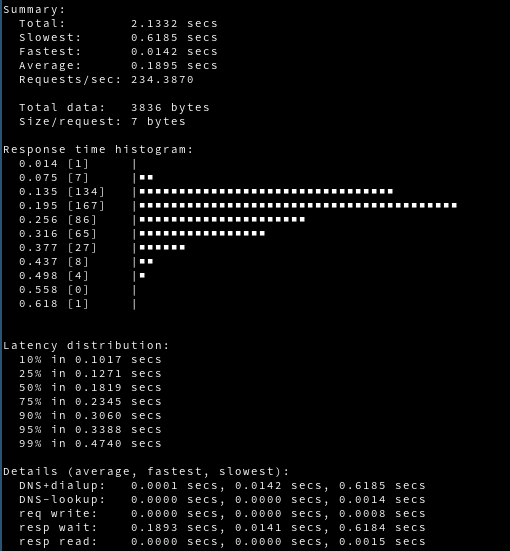
\includegraphics[width=100mm]{./thesis_images/real-fizz-buzz-2.png}
    \label{fig:real-fizz-buzz-2}
\end{minipage}
\end{center}
We can see that there is a bit of heavy variance in the response times of the
requests. On average the response time is about 0.1895 seconds which is more
than the previous case. This latency can be attributed to the cold start delay
during the scaling.

We can find an interesting corelation here between the scaling and the function
execution time. We start the system by maintaining a warm pool of 30 nodes for
higher number of requests. When we send out 50 requests at once, the system
scale up according to the alermanager rule that we defined. It can be seen from
the charts of the function rates and the execution duration how when the function 
is scaling up the execution time starts increasing steadily. This can be
referred from Figure \ref{fig:exec_time} and Figure \ref{fig:function_rate}.
These are charts from Grafana monitoring taken directly. In the former you can
see two plots under the execution time. The yellow one belongs to the time
spent on the start node and the lower one is of the function that tracks the
trace metrics of the same function. Although this adds some latency, this was
necessary to easy tracking of data. In the latter you can see the scaling rate
of the same node.

\begin{figure}[!h]
    \caption{Execution time - Composition with ephemeral storage}
    \centering
    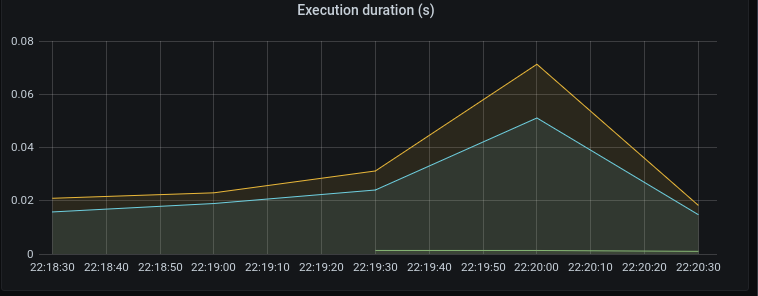
\includegraphics[width=80mm]{./thesis_images/exec_time.png}
    \label{fig:exec_time}
\end{figure}

\begin{figure}[!h]
    \caption{Scaling - Composition with ephemeral storage}
    \centering
    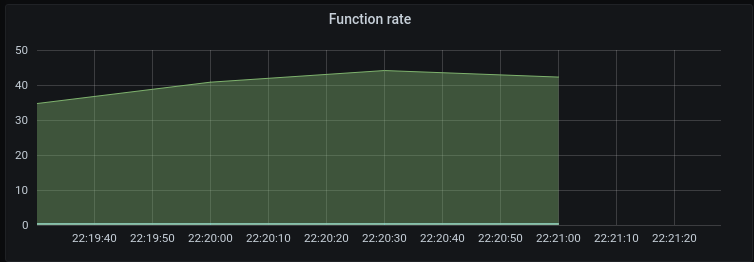
\includegraphics[width=80mm]{./thesis_images/function_rate.png}
    \label{fig:function_rate}
\end{figure}

\subsubsection{faas-flow with block storage}
\label{sec:org3546589}
The first scenario as was done with the previous workload, we use one request
per second for a minute HTTP request load as follows.
\begin{lstlisting}
hey -q 1 -c 1 -z 1m 'http://<server-ip>/function/fizz-buzz-minio'
\end{lstlisting}
In this case as well all the requests were successfully handled by the platform
(200OK response). The benchmark details from hey CLI is as in Figure \ref{fig:fizz-buzz-minio}

\begin{center}
   \begin{minipage}{\linewidth}
     \centering
     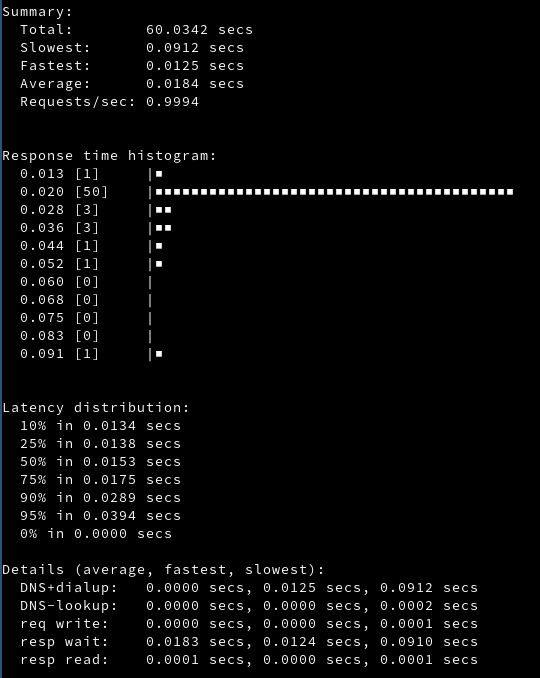
\includegraphics[width=100mm]{./thesis_images/fizz-buzz-minio-1.png}
     \captionof{figure}{Benchmark summary from hey for composition with block storage}
     \label{fig:fizz-buzz-minio}
   \end{minipage}
\end{center}

On an average the requests took 0.0184 seconds to complete the whole pipeline.
When we look at the function spans of each function, it can be seen that on
average the modifier node which represents the data modifier takes up quite a
bit of time along with the start node. This was shown as 0.00716s and 0.00932s respectively.

Similar to the above section, we repeat the experiment with a heavier load to
see how well the scaling is managed by the system. We get an average response
time of 0.3646 seconds. But in this experiment we had 3 timeouts. According to
the trace, there timeouts happened during the writing phase to the Minio. Figure
\ref{fig:fizz-buzz-minio-2} represents the benchmark information. The 3 requests
that exceeded 1 minute in execution are the ones that timed out.

\begin{center}
   \begin{minipage}{\linewidth}
     \centering
     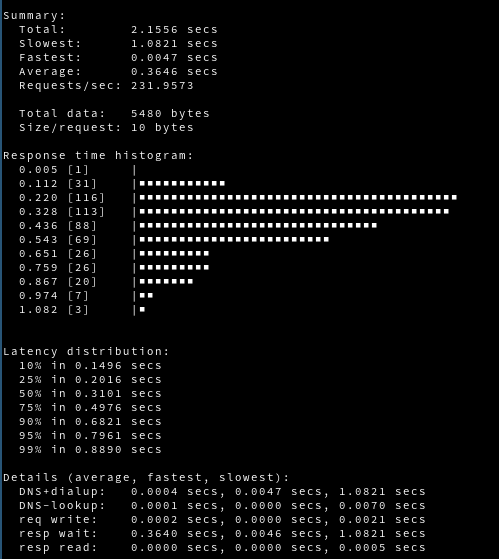
\includegraphics[width=100mm]{./thesis_images/fizz-buzz-minio-2.png}
     \captionof{figure}{Benchmark summary from hey for composition with block storage - higher load}
     \label{fig:fizz-buzz-minio-2}
   \end{minipage}
\end{center}

We do notice in this case as well a general spike in execution time when the
functions are getting scaled up after the warm pods we have kept on.

\subsubsection{Manual composition with block storage}
\label{sec:orgfa685bc}
For the manual composition, basically we wrote simple python functions of the
same functionality that would call each other via simple HTTP REST calls using
requests \hyperref[ref:73]{[73}] module. This is quite comparable with the recommended setup
recommended by some of the commercial FaaS offerings \hyperref[ref:20]{[20}].
The very same HTTP request load was applied first on manual composition to yield
a result as in Figure \ref{fig:fizz-buzz-manual}
\begin{lstlisting}
hey -q 1 -c 1 -z 1m 'http://<server-ip>/function/fizz-buzz-manual'
\end{lstlisting}
\begin{center}
   \begin{minipage}{\linewidth}
    \centering
    \captionof{figure}{Benchmark summary from hey for manual composition with block storage}
    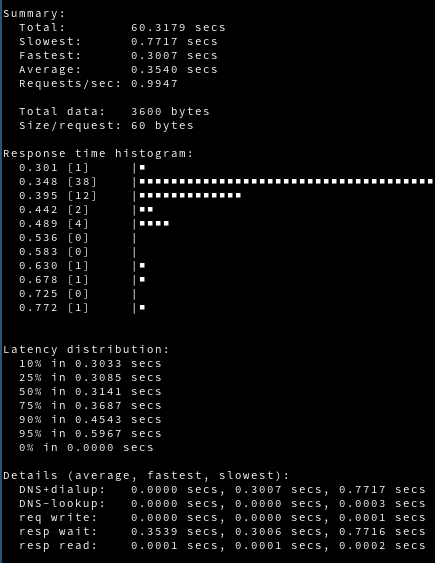
\includegraphics[width=100mm]{./thesis_images/manual-compo-1.png}
    \label{fig:fizz-buzz-manual}
   \end{minipage}
\end{center}

We can see that on average the function takes 0.33 seconds to complete a
request. Even in this case, we could see that all the requests were handled by
the system successfully. We could not measure spans of individual functions
exactly in this case because of the missing tracing infrastructure for this.

In the second phase of the test on this setup, as with the previous two cases, 
we mock above 200 requests per second on the manual composition pipeline. There
was a serious slowness in the scaling of the function in this scenario. The
function that is being called from another function did not scale well since it
is not being called simultaneously and would not trigger the Alertmanager rule.
Hence there were quite a few timeouts. 
\begin{center}
   \begin{minipage}{\linewidth}
    \centering
    \captionof{figure}{Benchmark summary from hey for manual composition with block storage and heavy load}
    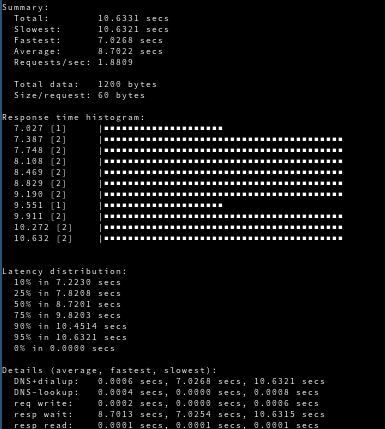
\includegraphics[width=100mm]{./thesis_images/manual-compo-2.png}
    \label{fig:manual-compo-2}
   \end{minipage}
\end{center}
Figure \ref{fig:manual-compo-2} shows the staggering slowness and network
clogging that happened during this test. On an average a request took around 8
seconds to complete a round trip. We could not notice clean scaling either in
this setup since only the coordinator functions kept scaling and not the
individual functions.

\subsubsection{Analysis}
\label{sec:orgef074e1}
Consolidating the above collection data, we create the Table \ref{tab:consolidation}
\begin{table}
\caption{Execution times of the compositions}
\label{tab:consolidation}
\centering
\resizebox{0.8\columnwidth}{!}{%
\begin{center}
\begin{tabular}{llrrrr}
Composition & Workload & Average & Fastest & Slowest & Timeouts\\
 &  & response & response & response & \\
 &  & time(s) & time(s) & time(s) & \\
 &  &  &  &  & \\
\hline
Manual & \textasciitilde{}1 request & 0.3540 & 0.3007 & 0.7717 & 1\\
Composition & per second &  &  &  & \\
\hline
Manual & \textasciitilde{}230 request &  &  &  & 4\\
Composition & per second & 8.7822 & 7.0268 & 10.6321 & \\
\hline
Faas-flow & \textasciitilde{}1 request &  &  &  & \\
with Object & per second & 0.0184 & 0.0125 & 0.0912 & 0\\
Store &  &  &  &  & \\
\hline
Faas-flow & \textasciitilde{}230 request &  &  &  & \\
with Object & per second & 0.3646 & 0.0047 & 1.0821 & 0\\
Store &  &  &  &  & \\
\hline
Faas-flow & \textasciitilde{}1 request &  &  &  & \\
with in-memory & per second & 0.0168 & 0.0129 & 0.0628 & 0\\
cache store &  &  &  &  & \\
\hline
Faas-flow & \textasciitilde{}230 request &  &  &  & \\
with in-memory & per second & 0.1895 & 0.0142 & 0.6185 & 0\\
cache store &  &  &  &  & \\
\hline
\end{tabular}
\end{center}

%
}
\end{table}

The initial analysis is driven from the first scenario of our testing setup.
When we look at the scenario with one request per second, we can understand that
on average each function takes an average of 0.0168 seconds in a setup with
faas-flow + ephemeral storage, 0.0184 seconds for faas-flow + block storages and
a staggering 0.3540s for the manual composition. These patterns were repeated
even when we increased the load to have heavy concurrent requests.

The problem that was noticed mainly with our proposed solution is the cold start
during the scaling up scenario. The reasons of this can be attributed to the
slow virtualization mechanism we are using. Although we did see that we had an
almost immediate scaling down when the load goes down. This is actually really
great for resource preservation.

With the setup using block storage, the modifier functions seem to be taking
longer which is the added latency of accessing the block storage. We could not
really achieve clean scaling up with the manual composition setup of the same.

\section{Related work}
\label{sec:org771b18b}
Serverless has gained a lot of attention and traction from the scientific
community in the past few years because of its massive implications in resource
conservation and innovative programming when one does not have to worry about
compute management anymore. The issues that were discussed in sessions above are
being studied by various studies and the most significant ones are worth noting.

Before getting into the studies that focus on the issues that was covered in
this paper, it is interesting to have a look at  a very recent literature review \hyperref[ref:53]{[53}]
. In the paper the authors analyze 112 different academic papers
and grey journals in
and around the paradigm of FaaS were analyzed. The researchers found a
staggering lack in the practicability of the work that were proposed by the
scientific community. Along with the lack of reusability and reproducability, it
was found that 88\% of these proposals were worked in and around AWS lambda,
which is not very universal as FaaS solution especially considering its vendor
locked in and closed source attributes. The study also mentions how most of
these works being done focus on unrealistic workloads that are not very common
in the production setups in the industry. The paper also says how the current
research lacks methods to chain and branch functions in a meaningful way.

In \hyperref[ref:54]{[54}], the authors interestingly look at the issues that the state of art
isolation mechanisms in FaaS infrastructure bring forward as was mentioned
earlier. These include the lack of security and the heavy cold start time. It
introduces faaslets, an alternate isolation policy to be used instead of
containers. With this, faaslets can share data across instances there by
reducing data transfer costs. In a contemporary study \hyperref[ref:55]{[55}], an
orchestration mechanism called TriggerFlow is introduced. It is a really
interesting tool to manage the lifecycle of a cloud function. In this smart
triggering system, function composition is allowed using Distributed Acyclic
Graphs(DAG) to define control flow and data flow in the pipeline. This has huge
potential as an idea, although currently the usability of the platform is
terrible and it can be quite bloated as a entry point to a FaaS system
especially since it is not a very elastic platform. In an older research, and
idea was proposed to schedule events based on tags which was quite similar. But
in a comparison, it is stated that the solution has a heavier memory footprint
than the former.


Cloudburst \hyperref[ref:2]{[2}] and SAND \hyperref[ref:3]{[3}] are projects that were mentioned in the previous
section. In the former, they suggest adding a key value cache along with
a limited DAG based language to specify the composition was specified before.
Although a very interesting idea, the issues with this systems were discussed
previously. SAND is a very interesting idea as well where they use a different
kind of isolation scheme to allow function composition as opposed to containers.

In yet another recent paper \hyperref[ref:4]{[4}], a theoretical model for a composition
language called serverless composition language(SPL) which lets the programmer
define function compositions(even can be higher order functions). This paper has
some very interesting formal foundations for serverless as a technology which
was used as a reference.

A very intriguing idea that has been proposed in the research community is to
change the programming model of serverless paradigms completely and introduce a
function shipping architecture for serverless. The idea is that it is suggested
that the way FaaS functions are designed is actually a architectural
anti-patterns that system designers make \hyperref[ref:13]{[13}]. Currently the
pattern can be referred as data shipping. Meaning that data is shipped to the
function as opposed to a function shipping architecture. An example for a
function shipping architecture would be procedures in databases where data is
not moved from its storage location. The reason why the data shipping pattern is
bad is because of the fact that across different storage layers and network
layers, there is a vast spectrum in the memory hierarchy which adds heavy
latencies. Shredder \hyperref[ref:56]{[56}] was a work towards adopting a function
coding pattern by adopting v8 isolation mechanism to boot up light weight
instances of the function near to the storage layer of the system. The problem
with this method is the fact that the current data loads are extremely
heterogeneous and it is hard to support this system on all the storage
platforms. But it is a very ambitious idea that has a lot of potential.

Coming to the domain of ephemeral scalable storage, Pocket is a very significant
project which was described in detail earlier. Anna KVS \hyperref[ref:57]{[57}], is a
similar idea which was adopted in the Cloudburst project. The tool was not
adopted in this project mostly because of the low elasticity the tool offers.


In InfiniCache \hyperref[ref:58]{[58}], a memory object cache is used to store the ephemeral
state in the system. It uses erasure coding and data backup to ensure high availability.
They try to get this system working on AWS lambda by connecting the runtime to a
priority based queue. In a very recent paper \hyperref[ref:61]{[61}], a shared filesystem is being
introduced that can be shared among the functions to transfer intermediate data
among themselves. Currently a very theoretical suggestion, FaasFS has the
potential to be an interesting mode of handling the intermediate data issue.

\section{Future work}
\label{sec:org057f67e}
The idea we presented here has a lot of potential for innovation mostly due to
its ease of adaptability and simplistic design. A very obvious improvement to
the platform would be the adaptation of a different isolation mechanism instead
of Docker containers. Since Docker containers are rather heavy as an isolation
mechanism, the cold start penalty in case of no warm nodes is still high. The
log during the scale up and down is due to this latency. A much lighter
isolation mechanism like v8 isolates \hyperref[ref:62]{[62}] might help in making the system faster. The
direction taken by FaaSM \hyperref[ref:54]{[54}] project is very applicable in this scenario. This only
tightens the security of the infrastructure since Docker containers can inherits
issues of the host operating system.

Furthermore, we plan on extending the project to provide better fault tolerance.
Since the workflow inherently supports conditional branching, we can extend the
API to accept callback functions in case of a function failure. With this the
developer can define the retry logic or the failure logic, thereby avoiding an
entire restart of the pipeline or worst - data corruption. We could also improve
the message queuing system to get an exactly one guarantee on the event handling.

Another improvement that we would like to make to our system is to introduce
intelligent data locality for the intermediate data. In the present
architecture, the data is being stored in the distributed cache which might
store it in any of the partition across the cluster. But we can introduce logic
that would place the data in the same machine as that of the function. This is a
very simplistic adaptation of the "porting function to the data logic". This
would reduce the latency spent of data transfer before the function invocation.

For developer friendliness, we can support multiple client libraries for the
application that would allow development of the workflow code in different
languages.

\section{Conclusion}
\label{sec:org1a09202}
In this paper, we analyzed a function composition solution and extended it to
use in-memory cache to store intermediate data between the functions. Our
initial thesis was that this would be a much better solution for big data
function pipelines, in which the developer would be bound to use a third party
block storage or pass via network both of which costs quite a bit on latency.
The proposed solution provides a very neat at efficient way to compose the
functions, reducing the latency of the manual orchestrations which has a higher
rate of gateway timeouts or the latency of block storages that adds the I/O
bottleneck. The system is very flexible allowing numerous operations while
composing the function like branching, looping, etc. This adds the possibility
of extending the platform for to support automatic roll-backs, error correction,
etc. Having said that, the system has limitations like slow scaling up at
certain instances due to the cold start latency. The system uses NATS streaming
for message queuing which is extremely simple and elastic but does not guarantee
exactly once semantics for the message delivery. Like was mentioned in the
section above, we believe that the improvements in the virtualization technology
can improve the latencies further.

\section{References}
\label{sec:orgb16bc2d}
\begin{enumerate}
\item \label{ref:1} \cite{bayliss09:_rollin_out_revol}
\item \label{ref:2} \cite{cloudburst}
\item \label{ref:3} \cite{sand}
\item \label{ref:4} \cite{formal}
\item \label{ref:5} \cite{containers}
\item \label{ref:6} \cite{aws}
\item \label{ref:7} \cite{economics}
\item \label{ref:8} \cite{lambdapricing}
\item \label{ref:9} \cite{lambdaintro}
\item \label{ref:10} \cite{compare_faas}
\item \label{ref:11} \cite{cloudflare}
\item \label{ref:12} \cite{edge}
\item \label{ref:13} \cite{onestep}
\item \label{ref:14} \cite{coldstart}
\item \label{ref:15} \cite{coldstartwar}
\item \label{ref:16} \cite{survey}
\item \label{ref:17} \cite{benchmark}
\item \label{ref:18} \cite{autodesk}
\item \label{ref:19} \cite{stepfunction}
\item \label{ref:20} \cite{mapreduce}
\item \label{ref:21} \cite{marla}
\item \label{ref:22} \cite{pocket}
\item \label{ref:23} \cite{crail}
\item \label{ref:24} \cite{olric}
\item \label{ref:25} \cite{consistent}
\item \label{ref:26} \cite{setnx}
\item \label{ref:27} \cite{multi}
\item \label{ref:28} \cite{cloudmulti}
\item \label{ref:29} \cite{namespace}
\item \label{ref:30} \cite{policies}
\item \label{ref:31} \cite{podsec}
\item \label{ref:32} \cite{clint}
\item \label{ref:33} \cite{montraclog}
\item \label{ref:34} \cite{systemd}
\item \label{ref:35} \cite{opentracing}
\item \label{ref:36} \cite{opentracdoc}
\item \label{ref:37} \cite{alerting}
\item \label{ref:38} \cite{dockerpop}
\item \label{ref:39} \cite{dockerpop}
\item \label{ref:40} \cite{dockerhub}
\item \label{ref:41} \cite{dockerref}
\item \label{ref:42} \cite{dockerever}
\item \label{ref:43} \cite{faassurvey}
\item \label{ref:44} \cite{faasprovider}
\item \label{ref:45} \cite{watchdog}
\item \label{ref:46} \cite{podscale}
\item \label{ref:47} \cite{plonk}
\item \label{ref:48} \cite{study}
\item \label{ref:49} \cite{datamodel}
\item \label{ref:50} \cite{pushgateway}
\item \label{ref:51} \cite{jaeger}
\item \label{ref:52} \cite{jaegerarch}
\item \label{ref:53} \cite{multivocal}
\item \label{ref:54} \cite{faasm}
\item \label{ref:55} \cite{triggerflow}
\item \label{ref:56} \cite{shredder}
\item \label{ref:57} \cite{anna}
\item \label{ref:58} \cite{infinicache}
\item \label{ref:59} \cite{github}
\item \label{ref:60} \cite{faasflow}
\item \label{ref:61} \cite{filesystem}
\item \label{ref:62} \cite{v8}
\item \label{ref:63} \cite{autoscaling}
\item \label{ref:64} \cite{olricdatastore}
\item \label{ref:65} \cite{msgpack}
\item \label{ref:66} \cite{nodeexp}
\item \label{ref:67} \cite{cadvisor}
\item \label{ref:68} \cite{helmcharts}
\item \label{ref:69} \cite{minio}
\item \label{ref:70} \cite{fizzbuzz}
\item \label{ref:71} \cite{hey}
\item \label{ref:72} \cite{minikube}
\item \label{ref:73} \cite{requests}
\end{enumerate}
\end{document}
